\documentclass[pdftex,a4paper,14pt,english,russian]{extarticle}

\usepackage[top=2cm,bottom=27mm,left=3cm,right=18mm]{geometry}
\usepackage[T2A]{fontenc}
\usepackage[utf8]{inputenc}
\usepackage[english,russian]{babel}
\usepackage[pdftex]{hyperref}
\usepackage{indentfirst}
\usepackage{titlesec}
\usepackage[pdftex]{graphicx}
\usepackage{amsmath}
\usepackage{amssymb}
\newcommand*\Laplace{\mathop{}\!\mathbin\bigtriangleup}
\usepackage[makeroom]{cancel}
\usepackage{ragged2e}

\usepackage{multirow}
\usepackage{algorithmic}
\usepackage[boxed]{algorithm}
\usepackage{tabularx}
\usepackage{xtab}
\usepackage{subfig}
\usepackage{hyphenat}
\usepackage{setspace}
\usepackage{fancyhdr}




% код программы - Листинг
\usepackage[usenames, dvipsnames]{color}
\definecolor{mygreen}{rgb}{0,0.6,0}
\usepackage{listings}
 \lstset{commentstyle=\color{mygreen},
 literate=
 	{~}{{\textasciitilde}}1
 	{а}{{\selectfont\char224}}1
 	{б}{{\selectfont\char225}}1
 	{в}{{\selectfont\char226}}1
 	{г}{{\selectfont\char227}}1
 	{д}{{\selectfont\char228}}1
 	{е}{{\selectfont\char229}}1
 	{ё}{{\"e}}1
 	{ж}{{\selectfont\char230}}1
 	{з}{{\selectfont\char231}}1
 	{и}{{\selectfont\char232}}1
 	{й}{{\selectfont\char233}}1
 	{к}{{\selectfont\char234}}1
 	{л}{{\selectfont\char235}}1
 	{м}{{\selectfont\char236}}1
 	{н}{{\selectfont\char237}}1
 	{о}{{\selectfont\char238}}1
 	{п}{{\selectfont\char239}}1
 	{р}{{\selectfont\char240}}1
 	{с}{{\selectfont\char241}}1
 	{т}{{\selectfont\char242}}1
 	{у}{{\selectfont\char243}}1
 	{ф}{{\selectfont\char244}}1
 	{х}{{\selectfont\char245}}1
 	{ц}{{\selectfont\char246}}1
 	{ч}{{\selectfont\char247}}1
 	{ш}{{\selectfont\char248}}1
 	{щ}{{\selectfont\char249}}1
 	{ъ}{{\selectfont\char250}}1
 	{ы}{{\selectfont\char251}}1
 	{ь}{{\selectfont\char252}}1
 	{э}{{\selectfont\char253}}1
 	{ю}{{\selectfont\char254}}1
 	{я}{{\selectfont\char255}}1
 	{А}{{\selectfont\char192}}1
 	{Б}{{\selectfont\char193}}1
 	{В}{{\selectfont\char194}}1
 	{Г}{{\selectfont\char195}}1
 	{Д}{{\selectfont\char196}}1
 	{Е}{{\selectfont\char197}}1
 	{Ё}{{\"E}}1
 	{Ж}{{\selectfont\char198}}1
 	{З}{{\selectfont\char199}}1
 	{И}{{\selectfont\char200}}1
 	{Й}{{\selectfont\char201}}1
 	{К}{{\selectfont\char202}}1
 	{Л}{{\selectfont\char203}}1
 	{М}{{\selectfont\char204}}1
 	{Н}{{\selectfont\char205}}1
 	{О}{{\selectfont\char206}}1
 	{П}{{\selectfont\char207}}1
 	{Р}{{\selectfont\char208}}1
 	{С}{{\selectfont\char209}}1
 	{Т}{{\selectfont\char210}}1
 	{У}{{\selectfont\char211}}1
 	{Ф}{{\selectfont\char212}}1
 	{Х}{{\selectfont\char213}}1
 	{Ц}{{\selectfont\char214}}1
 	{Ч}{{\selectfont\char215}}1
 	{Ш}{{\selectfont\char216}}1
 	{Щ}{{\selectfont\char217}}1
 	{Ъ}{{\selectfont\char218}}1
 	{Ы}{{\selectfont\char219}}1
 	{Ь}{{\selectfont\char220}}1
 	{Э}{{\selectfont\char221}}1
 	{Ю}{{\selectfont\char222}}1
 	{Я}{{\selectfont\char223}}1
 	{і}{{\selectfont\char105}}1
 	{ї}{{\selectfont\char168}}1
 	{є}{{\selectfont\char185}}1
 	{ґ}{{\selectfont\char160}}1
 	{І}{{\selectfont\char73}}1
 	{Ї}{{\selectfont\char136}}1
 	{Є}{{\selectfont\char153}}1
 	{Ґ}{{\selectfont\char128}}1
}
\newcommand{\angstrom}{\buildrel _{\circ} \over {\mathrm{A}}}
\numberwithin{equation}{subsection}
\pagestyle{fancyplain}
\fancyhf{}

\renewcommand{\headrulewidth}{0pt}
\rfoot{\fancyplain{}{\centering \thepage}} %нумерация страниц

\linespread{1.3}
\floatname{algorithm}{Алгоритм}

\addto\captionsrussian{ \renewcommand{\contentsname}{ СОДЕРЖАНИЕ}}
\addto\captionsrussian{ \renewcommand\refname{СПИСОК ИСПОЛЬЗОВАННЫХ ИСТОЧНИКОВ}}

% прилоение
\addto\captionsrussian{ \renewcommand\appendixname{Приложение}}
\makeatletter
\def\redeflsection{\def\l@section{\@dottedtocline{1}{1.5em}{7.8em}}}
\renewcommand\appendix{\par
\setcounter{section}{0}%
\setcounter{subsection}{0}%
\def\@chapapp{\appendixname}%
\addtocontents{toc}{\protect\redeflsection}
\def\thesection{\appendixname\hspace{0.2cm}\@arabic\c@section}}
\makeatother
% /прилоение
% new commands
\newcommand\sign[1]{sign(#1)}



% подрисуночная подпись

\addto\captionsrussian{\renewcommand{\figurename}{Рисунок}}
\makeatletter
\long\def\@makecaption#1#2{%
  \vskip\abovecaptionskip
  \hbox to\textwidth{\hfill\parbox{1\textwidth}{\centering #1 - #2}\hfill}
  \vskip\belowcaptionskip}
\makeatother

% новый уровень
\titleclass{\subsubsubsection}{straight}[\subsection]

\newcounter{subsubsubsection}[subsubsection]

\renewcommand\thesubsubsubsection{\thesubsubsection.\arabic{subsubsubsection}}
\renewcommand\theparagraph{\thesubsubsubsection.\arabic{paragraph}}
\renewcommand\thesubparagraph{\theparagraph.\arabic{subparagraph}}

\titleformat{\subsubsubsection}
  {\normalfont\normalsize\bfseries}{\thesubsubsubsection}{1em}{}
\titlespacing*{\subsubsubsection}
{0pt}{3.25ex plus 1ex minus .2ex}{1.5ex plus .2ex}

\makeatletter
\renewcommand\paragraph{\@startsection{paragraph}{5}{\z@}%
  {3.25ex \@plus1ex \@minus.2ex}%
  {-1em}%
  {\normalfont\normalsize\bfseries}}
\renewcommand\subparagraph{\@startsection{subparagraph}{6}{\parindent}
  {3.25ex \@plus1ex \@minus .2ex}%
  {-1em}%
  {\normalfont\normalsize\bfseries}}
\def\toclevel@subsubsubsection{4}
\def\toclevel@paragraph{5}
\def\toclevel@paragraph{6}
\def\l@subsubsubsection{\@dottedtocline{4}{7em}{4em}}
\def\l@paragraph{\@dottedtocline{5}{10em}{5em}}
\def\l@subparagraph{\@dottedtocline{6}{14em}{6em}}
\@addtoreset{subsubsubsection}{section}
\@addtoreset{subsubsubsection}{subsection}
\@addtoreset{paragraph}{subsubsubsection}
\makeatother
\setcounter{secnumdepth}{6}
\setcounter{tocdepth}{6}

% названия с красной строки
\titlespacing*{\section}{\parindent}{1ex}{1em}
\titlespacing*{\subsection}{\parindent}{1ex}{1em}
\titlespacing*{\subsubsection}{\parindent}{1ex}{1em}
\titlespacing*{\subsubsubsection}{\parindent}{1ex}{1em}
%добавить точку после номера
\makeatletter
\renewcommand{\@seccntformat}[1]{\indent \csname the#1\endcsname.\quad}
\makeatother

\begin{document}
\begin{titlepage}
  \begin{center}
    % \textsc{\small Министерство образования Республики Беларусь}\\[0.5cm]
    \textsc{\small \large федеральное государственное бюджетное образовательное
    учреждение высшего образования "московский государственный университет им. Ломоносова"}\\[0.3cm]
    \textsc{\large Физический факультет}\\[0.3cm]
    \textsc{\large кафедра оптики, спектроскопии и физики наносистем}\\[0.5cm]

    \begin{minipage}{\textwidth}
      \begin{flushleft}

      \end{flushleft}
    \end{minipage}\\[0.5cm]

    \textsc{\large  магистерская диссертация}\\[0.5cm]
    \textbf{\large Двух- и трехкристальная дифрактометрия в исследовании
    пьезоэлектрических кристаллов в условиях воздействия электрического поля}\\[1.5cm]


    \begin{minipage}{\textwidth}
      \begin{flushright}
        Выполнил студент группы 241М \hspace*{2.1cm} \\
        Аткнин И. И.\underline{\hspace*{4.6cm}}\\[0.5cm]
        Научный руководитель: к.ф.-м. н. \hspace*{1.8cm} \\
        Марченков Н. В. \underline{\hspace*{3.7cm}}\\[0.5cm]
        Научный руководитель: к.ф.-м. н., доцент\\
        Стремоухов С. Ю. \underline{\hspace*{3.7cm}}\\[0.5cm]
      \end{flushright}
    \end{minipage}\\[1.5cm]


    \begin{minipage}{\textwidth}
      \begin{flushleft}
        \textit{Допущена к защите 31.05.2017}\\
        Зав. кафедрой \underline{\hspace*{4.5cm}}\\
      \end{flushleft}
    \end{minipage}\\[1.5cm]

    \vfill
    \textsc{\small Москва\\ 2017}
  \end{center}
\end{titlepage}

\setcounter{page}{2}

\titleformat*{\section}{\centering\bfseries\Large}
\tableofcontents
\titleformat*{\section}{\bfseries\Large}


\newpage
% ---------------------section 1 -----------------------
  \section*{\centering ВВЕДЕНИЕ}
  \addcontentsline{toc}{section}{\protect\numberline{}ВВЕДЕНИЕ}%
  \section*{ВВЕДЕНИЕ}
\addcontentsline{toc}{section}{Введение}

В последние время, благодаря интенсивному развитию информационных технологий, процесс снятия изображения и/или видео и его хранение достаточны просты. Более того, на сегодняшний момент весьма недороги. Поэтому все большее распространение получают системы наружного наблюдения, системы индексации видео, системы автомобильной безопасности и т.д.

Целью данного дипломного проекта являются описание и разработка обобщенного фреймворка для захвата людей на изображении и оценки их позы, основанного на графических структурах (pictorial structures).

В современном мире обширнейшие электронные коллекции изображений и даже видео --- не редкость. Оцифровка и хранение больших объемов визуальных материалов не является проблемой с технической точки зрения.

До недавнего времени традиционным считался поиск визуальной информации, опирающийся на индексирование текстовых описаний, ассоциированных с изображением или видео.

При очевидной необходимости организации доступа к визуальной коллекции посредством поиска по текстовой информации, такой подход представляется недостаточным. Неоднозначность соответствия между визуальным содержанием и текстовым описанием снижает показатели точности и полноты поиска.

В связи с этим возникает проблема организации доступа к современным электронным коллекциям изображений и видео и использованием комплекса средств --- как текстовых описаний, так и характеристик визуального содержания, простейших типа цветовой гаммы и более сложных, связанных с распознаванием образов. Текстовое описание и визуальная поисковая информации дополняют друг друга, обеспечивая возможность разностороннего поиска. Часть поисковой информации предоставляют выходные данные программного обеспечения, разработанного в рамках данного дипломного проекта. Используя ее, можно разработать поисковую систему для систем наружного наблюдения, которая позволит выполнять запросы вида: ``показать кадры определенного участка, на которых присутствует хотя бы один человек в заданное время''.

Другой областью применения результатов проекта являются системы видеонаблюдения для обеспечения безопасности и охраны. Такие системы способны определить, где находится субъект, в каком он направлении движется и оценить в какой позе он находится. Это позволяет значително уменьшить нагрузку с оператора данной системы, так как в этом случае ему не надо следить постоянно за всеми камерами одновременно. Ведь с помощью автоматического захвата людей на видео, поступающего с камер наблюдения, например, можно реализовать функцию системы, которая будем сигнализировать в том случае, если на обозреваемом участке появился какой-либо субъект.

Также можно реализовать функцию поиска определенных действий на видео, например, поиск всех кадров, на которых присутствует человек с поднятыми руками.

До недавнего времени методы захвата людей не могли быть применены в широком спектре задач из-за отсутствия эффективных универсальных алгоритмов и подходов. Здесь мы пытаемся продемонстрировать последние достижения этого раздела знаний в области компьютерного зрения. В \cite{andriluka09} показано на эксперементах, что этот подход превосходит другие методы на трех наборах тестовых данных. Следует особо подчеркнуть, что другие методы разработаны с учетом специфики входных данных. Это наглядно демонстрирует такое свойство демонстрируемого метода, как обобщенность.

Несмотря на это, предоставленная модель на удивление проста. Это стало возможным, по нашему мнению, благодаря двум ключевым компонентам:
\begin{itemize}
  \item строго дифференцирующей модели представления, которая позволяет надежно захватывать отдельные части объекта на изображении,
  \item и моделированию конфигурации объекта с помощью графических структур.
\end{itemize}

В данном дипломном проекте рассматривается современный метод захвата людей на изображении и оценки их позы, основанный на графических структурах, а также производится его реализация.

\newpage

  \newpage
\section{Литературный обзор}
  \subsection{Атомный фактор рассеяния}
    
Рентгеновское излучение, взаимодействуя с электронами атомов вещества рассеивается.
Протоны (ядра атомов) в рассеянии рентгеновских лучей практически не участвуют, т.к.
амплитуда электромагнитной волны, рассеянной заряженной частицей,
 обратно пропорциональна ее массе - формула Томсона \cite{iveronova1972}. Величина такого рассеяния
 зависит от количества электронов в атоме.  Тяжелые металлы,
 например свинец, Pb (Z = 82), рассеивают рентгеновское излучение сильнее легких,
 таких как Ni (Z = 28) или  Co (Z = 27), а такие атомы, как He или H – прозрачны
 для рентгеновского излучения.  Атомный множитель $f$ (атомный фактор рассеяния) определяется
как отношение амплитуды волны, рассеянной одним атомом, к амплитуде волны, рассеянной
одним свободным электроном. Действительно, если в какой либо точке пространства сосредоточено
$Z$ электронов, то заряд этой группы равен $Q = Z\cdot e$, а масса $M = Z \cdot m_e$.

На рис. \ref{ris:atom_factor} представлена диаграмма направленности атомного
фактора лантана в зависимости от угла. Размеры атома соизмеримы с длиной волны
рентгеновских лучей, поэтому между волнами рассеянными отдельными электронами, возникает
разность фаз. Это разность фаз равна нулю только при $2 \theta = 0$, поэтому структурный
фактор зависит от $\theta$ и $\lambda$. Максимальная величина, которая равна $Z$,
 наблюдается в случае рассеяния вперед.

\begin{figure}[H]
  \centering
  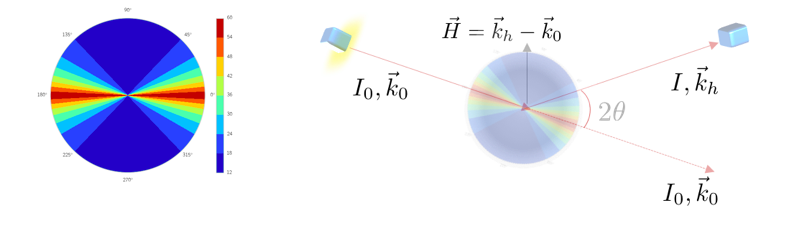
\includegraphics[width=0.9\textwidth]{images/atom_factor.png}
  \caption{ (Слева) фактор рассеяния для атома лантана (La, N = 57), (справа)
  схема расположения векторов для падающей и рассеянной волн}
  \label{ris:atom_factor}
\end{figure}

Приближенное выражение для расчета атомного фактора рассеяния
представляется \cite{International_Tables} в виде выражения:

\begin{equation}
  f_0 = \sum_{i=1}^{4} \cdot a_i e^{ -b_i (\frac{sin \vartheta_B}{\lambda})^2} + C
 \end{equation}
где $a_i$, $b_i$ и $c$ - коэффициенты Кромер-Манна для бездисперсионного канала рассеяния атомами решетки,
ограничением является $0<\frac{sin\vartheta}{\lambda}<2.0 \angstrom ^{-1}$.
 Характерная зависимость структурного фактора от угла рассеяния и длины волны
для атомов входящих в состав кристалла LGT (La, Ga, Ta, O) представлена на рис. \ref{ris:atom_factor_GaLaTa}.

\begin{figure}[H]
  \centering
  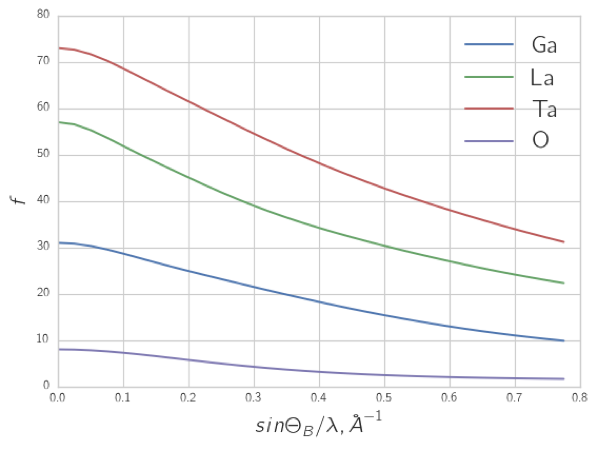
\includegraphics[width=0.6\textwidth]{images/atom_factor_GaLaTa.png}
  \caption{ Атомный фактор рассеяния для атомов: галлия (Ga), лантана (La), тантала (Ta) и  кислорода (O)}
  \label{ris:atom_factor_GaLaTa}
\end{figure}

При расчете интенсивности рассеяния атомом необходимо учитывать факт,
что все электроны связаны между собой, таким образом необходимо записывать
уравнение движение связанного электрона по действием падающего излучения.
Если атом многоэлектронный, то амплитуда рассеянной волны равна сумме амплитуд волн,
рассеянных всеми электронами атома, в результате структурный фактор \cite{iveronova1972}:

\begin{equation}
  f = f_0 + f^{'} + i f^{''}
 \end{equation}
\noindent
где, $f_0$ - атомный фактор рассеяния, рассчитанный без учета сил связи электронов
 с ядром, а $f^{'}$ и $f^{''}$ - дисперсионные поправки \cite{f0f1f12},
 первая из которых учитывает дополнительное рассеяние,
а вторая - дополнительное поглощение вблизи собственных частот колебаний электронов в атоме.

 \begin{figure}[H]
   \centering
   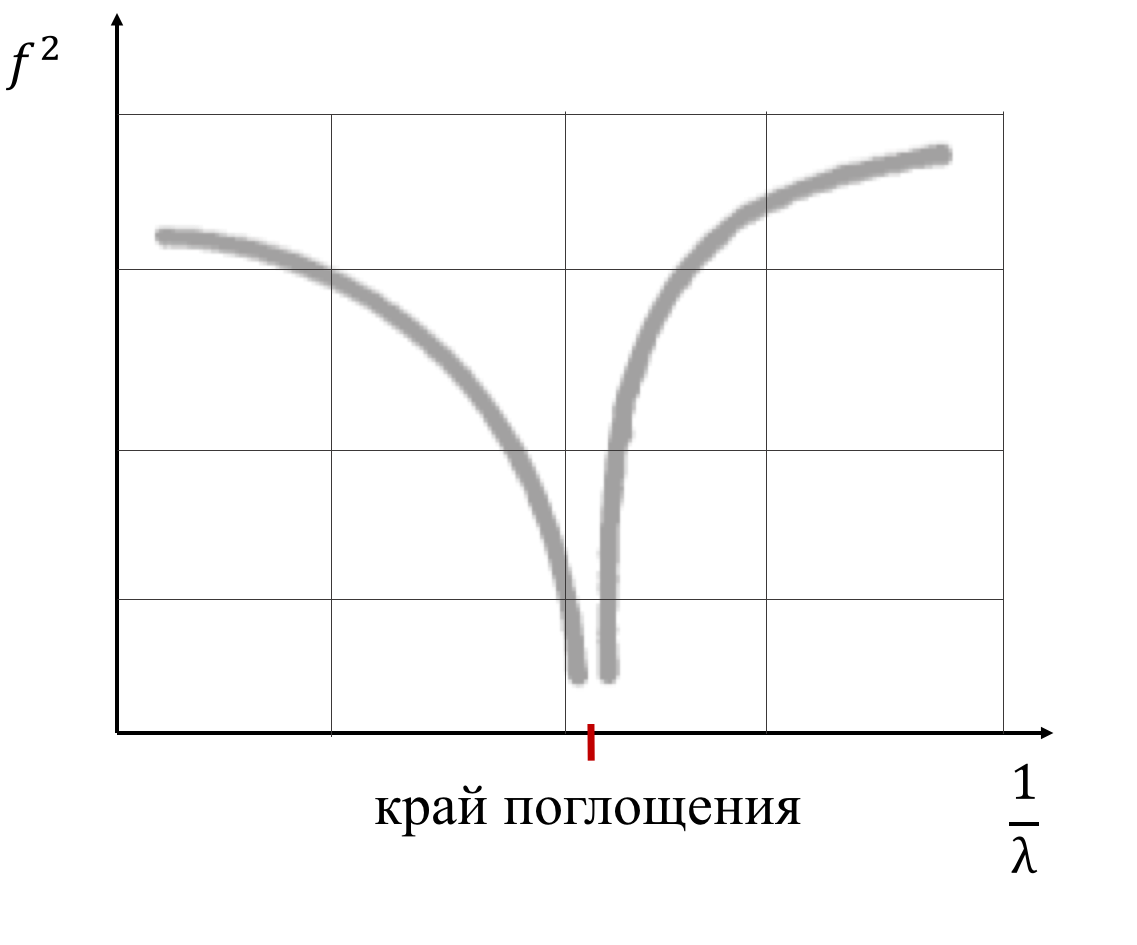
\includegraphics[width=0.4\textwidth]{images/dispers_f.png}
   \caption{ Схематичная зависимость квадрата атомного фактора $f^2 = (f_0 + f^{'})^2 + (f^{''})^2 $ от
   длины волны $\lambda$ вблизи края поглощения}
   \label{ris:dispers_f}
 \end{figure}

Важной особенностью является факт того, что дисперсионные поправки $f^{'}$, $f^{''}$
практически не зависят от длины волны, но зависят от энергии. Так как $f_0$ уменьшается
с ростом угла рассеяния, дисперсионные поправки начинают играть роль при больших углах $\theta$.

  \subsection{Структурный фактор рассеяния}
    \label{sec:structure_factor}
Атомы решетки, взаимодействуя с рентгеновским излучением, рассеивают его.
Если в элементарной ячейке более одного атома, волны от разных атомов,
 интерферируя между собой, вносят вклад в общую картину рассеяния,
 ослабляя или усиливая ее.

 \begin{figure}[H]
   \centering
   \subfloat[]{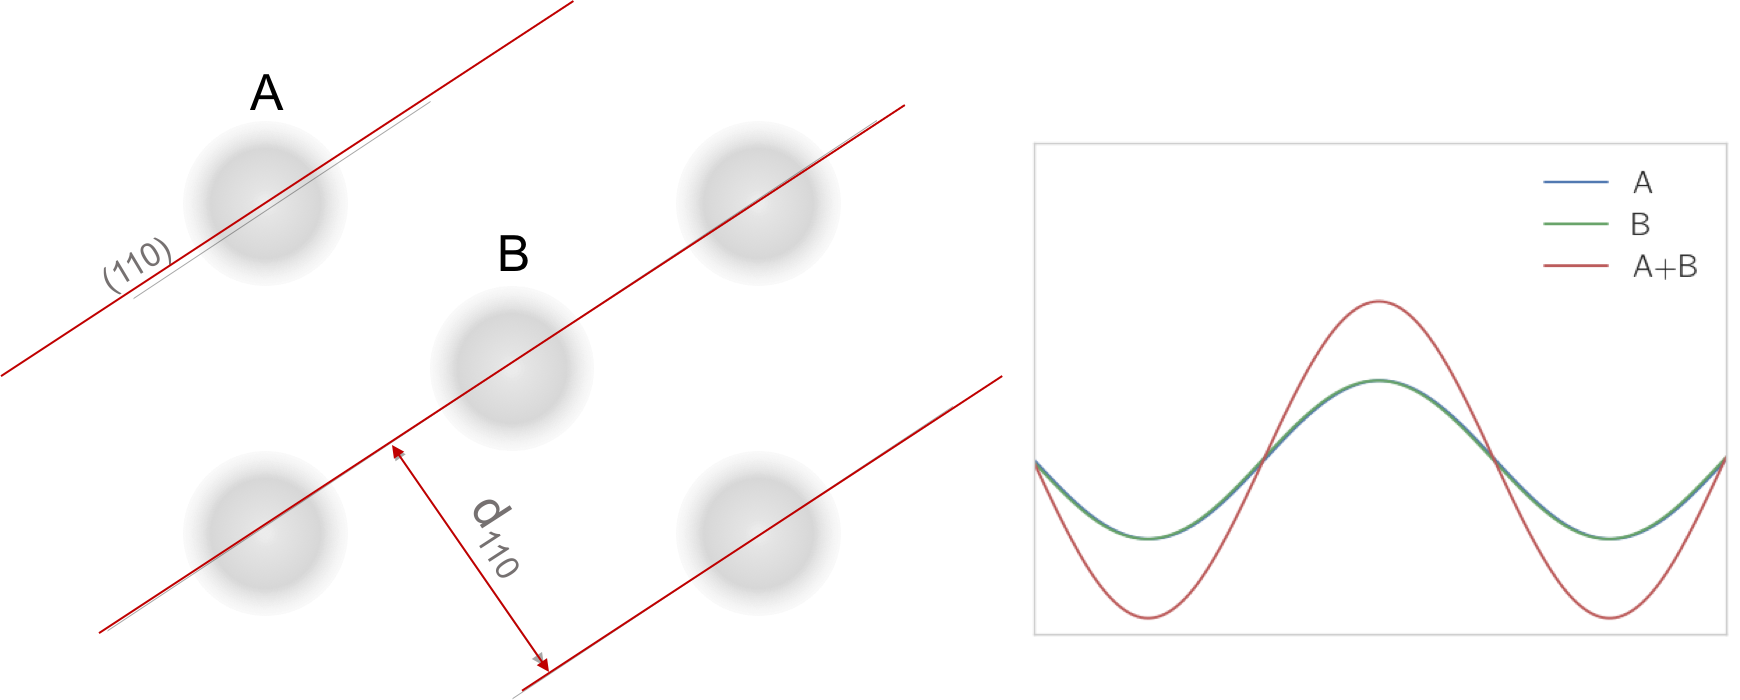
\includegraphics[width=0.45\textwidth]{images/interference_construct.png}}
   \hfill
   \subfloat[]{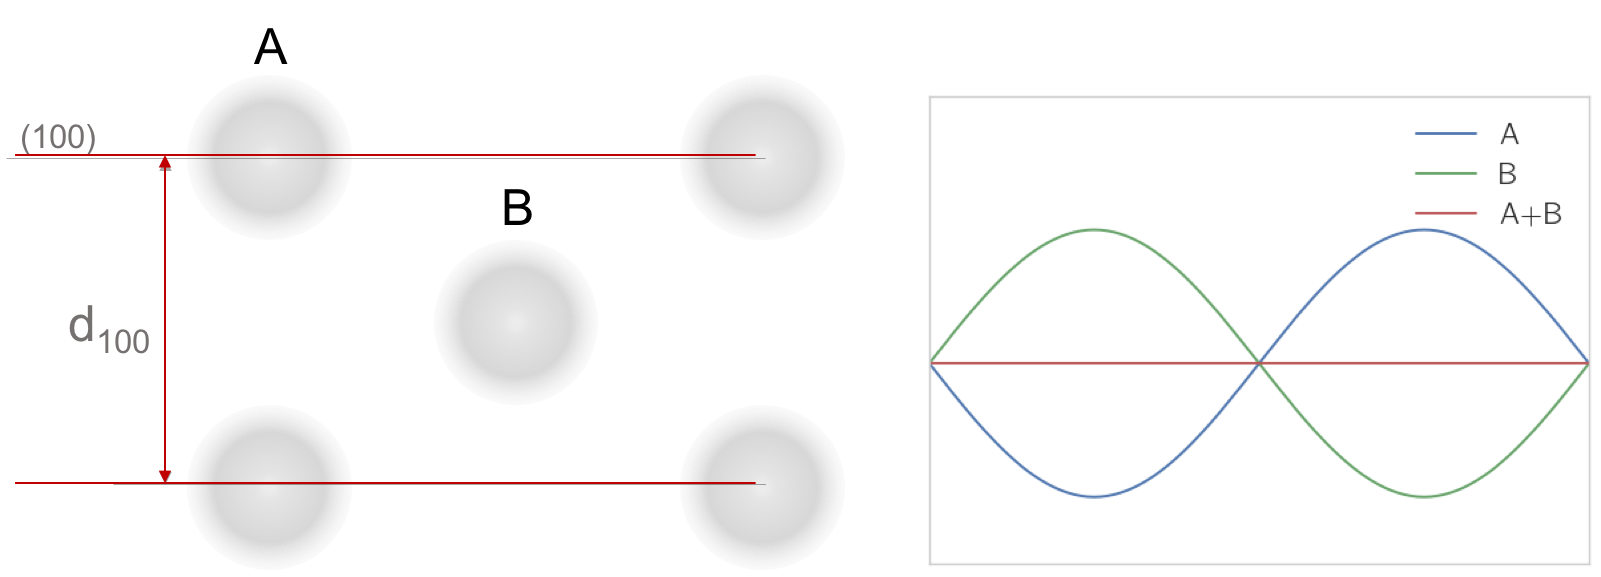
\includegraphics[width=0.45\textwidth]{images/interference_destruct.png}}
   \caption{Примеры интерференции двух волн, отраженных различными системами атомных плоскостей для случая
   конструктивной (a) и деструктивной (b) интерференции}
   \label{ris:interference_by_plate}
 \end{figure}

Рассеяние от набора атомов характеризуется структурным фактором, определяемым векторным
 сложением фаз по всем N атомам элементарной ячейки:

 \begin{equation}
   F = \sum_{n} f_n e^{ i\vec{h}\vec{r}_n} =   \sum_{n} f_n \cdot e^{-i\phi_n},
   \label{eq:F_factor}
  \end{equation}
\noindent
где $\phi_n = 2 \pi (hx_n+ky_n+lz_n)$;  $h, k, l$ - индексы Миллера; $x, y, z$ - относительные координаты
атомов в элементарной ячейке.

В соответсвии с \ref{eq:F_factor} в качестве примера был произведен расчет трехмерной ($hkl$) -
карты струкутрного фактора (рис. \ref{ris:hkl_LGT_SI}).
Цветом изображена величина структурного фактора для разных
 индексов плоскостей отражения для кристаллов LGT и Si.
 В таком представлении просматривается периодичность образования запрещенных
 рефлексов в кубическом кремнии. В кристалле LGT запрещенных (синий цвет)
  индексов для отражения на порядок меньше, связанно это с более низкой
  симметрией кристалла.

  \begin{figure}[h]
    \centering
    \subfloat[]{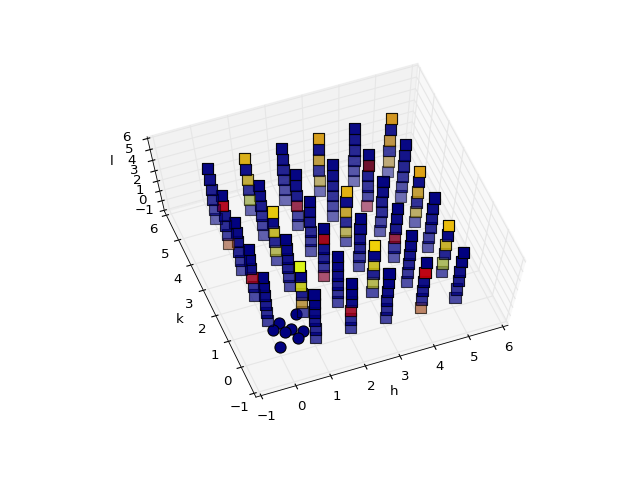
\includegraphics[width=0.5\textwidth]{images/hkl_Si.png} \label{ris:hkl_LGT_SI_a}}
    \hfill
    \subfloat[]{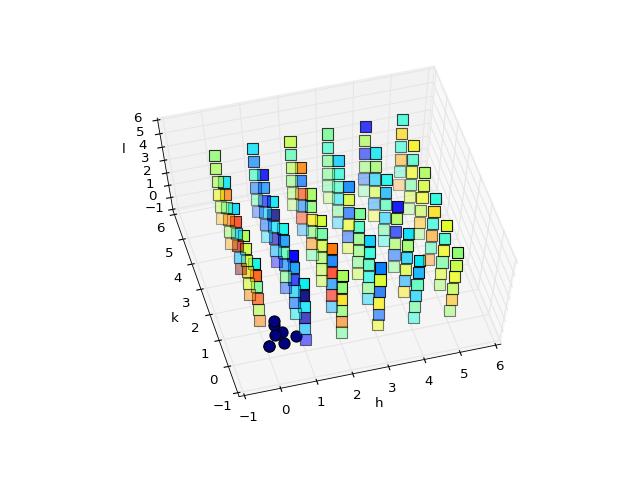
\includegraphics[width=0.5\textwidth]{images/hkl_LGT.png} \label{ris:hkl_LGT_SI_b}}
    \caption{Карта распределения величины структурного фактора
    (цвет соответствует его величине) в координатах индексов Миллера для кристалла Si (a) и LGT (b)}
    \label{ris:hkl_LGT_SI}
  \end{figure}

  \subsection{Влияние температуры. Тепловой фактор Дебая - Валлера}
    \subsection{Влияние температуры. Тепловой фактор}

При расчете структурных амплитуд рассеяния необходимо учитывать
тепловые колебания атомов в решетке. Предположим, что атомы колеблется около положения
равновесия независимо друг от друга, тогда это эквивалентно увеличения радиуса атома,
что приводит к более быстрому спаду функции атомного рассеяния с ростом угла рассеяния.
С другой стороны эффективное увеличение радиуса атома, очевидно должно зависеть от
величины среднеквадратичного смещения смещения атома  $<u^2>$ из положения равновесия.
Также для простоты предположим, что период тепловых колебаний атомов намного больше периода
колебаний падающего излучения, тем самым мы можем считать атом неподвижным в момент рассеяния,
т.е. пренебречь эффектом Доплера.

Таким образом структурный фактор необходимо усреднить за время наблюдения по всем возможным отклонениям
\begin{equation}
  F_T = \left\langle \sum_{n} f_n \cdot  e^{-i\vec {h} \cdot (\vec{r_n}+ \vec{u}(t))} \right\rangle =  \sum_{n} f_n \cdot  e^{-i\vec {h} \cdot \vec{r_n}}  \left\langle e^{-i \vec{h} \cdot \vec {u}(t)  } \right\rangle
 \end{equation}

где $\vec{u(t)}$ - отклонение атома во времени, $\vec{r_n}$ - положение атома $n$
в идеальной ячейки, суммирование производится, по всем атомам элементарной ячейки.
$\vec{h}$ - вектор обратной решетки, $|\vec{h}| = 2 \pi / d = $ где $d$ - межплоскостное расстояние.

Разложим экспоненту, содержащую параметр отклонения, в ряд Тейлора:

\begin{equation}
  \left\langle e^{-i \vec{h} \cdot \vec {u}(t)  } \right\rangle = 1 - i  \left\langle \vec{h} \cdot \vec {u} \right\rangle - \frac{1}{2} \left\langle (\vec{h} \cdot \vec {u})^2 \right\rangle+ \ldots
 \end{equation}

 Cреднее значение всех членов нечетной степени будет тождественно равно нулю.
Учитывая,  $ \left\langle (\vec{h} \cdot \vec {u})^2 \right\rangle = q^2 <u^2> <cos(\theta)> = \frac{1}{2}<u^2>h^2$, преобразуем ряд,

\begin{equation}
1 - i  \left\langle \vec{h} \cdot \vec {u} \right\rangle - \frac{1}{2} \left\langle (\vec{h} \cdot \vec {u})^2 \right\rangle+ \ldots = e^{-\frac{1}{2} <u^2> h^2}
 \end{equation}


 \begin{equation}
   F_T =  \sum_{n} f_n \cdot  e^{-i\vec {h} \cdot \vec{r_n}}  e^{-B (\frac{sin\theta_B}{\lambda} )^2 }
  \end{equation}

 где $B = 8 \pi^2 <u^2>$ - температурный коэффициент Дебая - Валлера,
 $(\frac{h}{4\pi})^2=(\frac{sin\vartheta_B}{\lambda})^2$ -
 вектор вектор обратной решетки или вектор рассеяния. Обычно температурный коэффициент
 находится в пределах от $0.20 \angstrom ^2$ до $3.0 \angstrom ^2$.

 Здесь мы ограничились тем, что все колебания в кристалле изотропные
 (изотропное гармоническое приближение), в более общем случае
 температурный коэффициент определяется тенором третьего порядка \cite{Willis1975}.
 В большинстве случаев гармоническое приближение дает адекватное описание, однако при описании
 атомных колебаний в области высоких температур, когда амплитуда колебаний сопоставима с расстоянием
 между соседними атомами, гармоническое приближение некорректно, в этом случае нужно учитывать ангармонические
 поправки \cite{kibalin2015}.
 \begin{equation}
   <u^2> = <u^2_{harm}> (1+2\gamma \alpha T)
  \end{equation}
  где, $\gamma$ - константа Грюнайзена, $\alpha$ - объемный коэффициент теплового расширения, $T$ - температура.
  В случае возрастания температуры кристалла, интенсивность Бреговского рефлекса будет уменьшаться,
  но угловая полуширина отраженной кривой постоянной останется прежней.

 Кроме теплового фактора Дебая-Валлера (динамического), существует и статическая составляющая,
 величина которой в первую очередь зависит от концентрации дефектов в образце,
 такой вклад меньше зависит от температуры, поэтому проведение температурных измерений
 обычно позволяет разделить статический и динамический вклады.


% Разложим второе слагаемое в ряд Тейлора, тогда среднее значение всех членов нечетной степени
% будет тождественно равно нулю. Ограничившись вторым порядком разложения, получим:
%
% \begin{equation}
%   F_T = F \cdot  \left(1 - 4 \pi^2 <u^2> \left( \frac{h}{a} + \frac{k}{b} + \frac{l}{c}\right)^2 \right)
%  \end{equation}

% Мерой смещения атомов при тепловых колебаниях служит
% их среднеквадратичная амплитуда:
% \begin{equation}\label{eq:debay}
%   <u^2> = \frac{9\hbar^2 T}{m k_B \Theta_D^2}
%  \end{equation}
% где $\hbar$ - постоянная Планка, $k_B$ - постоянная Больцмана, $\Theta_D$ - температура Дебая.
% Величина $B$ может варьироваться в диапазоне от $1 \angstrom $ до $ 100\angstrom $.
%
% В случае возрастания температуры кристалла, интенсивность Бреговского рефлекса будет уменьшаться,
% но угловая полуширина отраженной кривой постоянной останется прежней. Удивительным является то, что
% удается получить достаточно узкие кривые отражения от кристалла в котором атомы случайным
% образом смещены относительно равновесных положений, относительное изменение расстояния
% между соседними атомами может составлять до 10$\%$ при комнатной температуре.

  % \subsection{Кинематическая теория рассеяния}

  \subsection{Динамическая теория рассеяния}
    \subsubsection{Симметричная схема дифракции}
        При рассмотрении большинства физических процессов, задействованных
  в методах исследования структуры веществ с помощью рентгеновских лучей,
  используется математический аппарат волновой оптики.
  Плоская монохроматическая волна, распространяющая в вакууме, изображена на рисунке ~\ref{ris:plane_wave_vacuum},
  амплитуда плоских волн в вакууме $E_0$ не меняется с удалением от
  источника (в отличии от сферических или цилиндрических). В приближении плоской волны,
  плотность потока энергии, переносимой волной через единицу площади неизменна на любом расстоянии от источника.

  \begin{figure}[H]
    \centering
    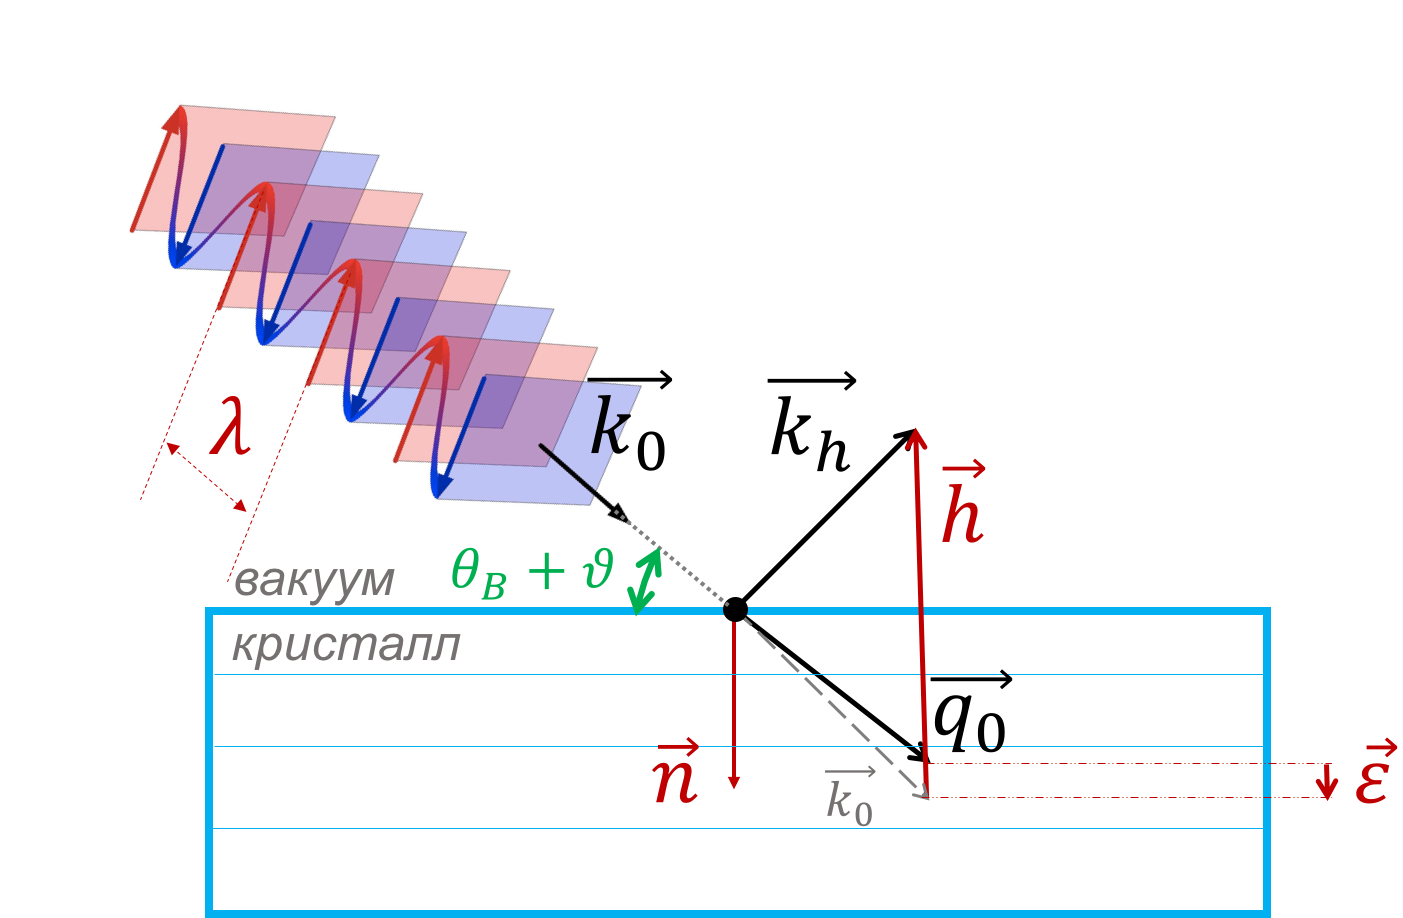
\includegraphics[width=0.8\textwidth]{images/plane_wave_vacuum.png}
    \caption{Схема к описанию динамической теории дифракции рентгеновского излучения с кристаллом.
      $\vec {k}$ - волновой вектор в вакууме; $\vec {q}$ - волновой вектор в среде;
     $0$ - коэффициент для обозначения падающей волны, а $h$ -  дифрагированной волны; $\vec{h}$ - вектор
     обратной решетки ($|h|=2\pi/d$); $\vec{n}$ - вектор нормали к поверхности, направленный внутрь объема;
     $\lambda$ - длина волны волнового вектора; $\vec{\varepsilon}$ - вектор аккомодации, характеризующий изменение
     волнового вектора в среде из-за преломления; $\vartheta$ - угол падения излучения на кристалл, для данного
     случая угол совпадает с углом Брегга $\vartheta = \theta_B$, т.к.  $\vec {k}_0 + \vec{h} = \vec {k}_h $}
    \label{ris:plane_wave_vacuum}
  \end{figure}

Рентгеновские лучи, как и видимы свет, распространяются параллельно и преломляются при
прохождении через границу раздела двух сред с разной оптической плотностью.
 Преломление рентгеновских лучей намного слабее, чем у видимого света, причем
 абсолютный показатель преломления рентгеновских лучей практически во всех средах
 практический одинаков и настолько близок к единице, что их преломление не удавалось обнаружить
 в течение тридцати лет после открытия рентгеновских лучей \cite{fetisov2007}, более того
 для рентгеновских лучей вакуум оказывается оптически наиболее плотной средой и луч
 при переходе в конденсированную среду увеличивает угол с нормалью к поверхности раздела сред ($n_{refr} \approx 1-10^{-5}$ ).
 Таким образом, волновой вектор, распространяющийся в вакууме отличается от своего продолжения в
 среде, но тангенциальная составляющая при переходе из одной среды в другу, в соответствии с теорией о циркуляции, сохраняется \cite{landau_8_1992}.

 \begin{equation}
   \vec{q}_0 = \vec{k}_0 + \varepsilon k_0 \cdot \vec{n}
  \end{equation}

Квадрат вектора,

\begin{equation}
   q_0^2 = k_0^2 + 2k_0^2 \varepsilon \cdot \gamma_0 + \cancelto{0}{k_0^4  \varepsilon^2}
   \label{eq:k_0_squred}
 \end{equation}

  где, $\gamma_0 = \cos(\vec{k}_0 \textasciicircum \vec{n})$ - косинус угла между вектором $\vec{k}_0$ и нормалью к поверхности кристалла,
  последним слагаемым можно пренебречь в силу его малости ($\sim 10^{-6}$).
  Волновой вектор дифрагированной волны, в соответствии с условием Брегга,

  $$\vec{k}_h = \vec{k}_0+\vec{h}$$

  \begin{equation}
     k_h^2 = \vec{k}_0^2+2k_0^2 \varepsilon \cdot \gamma_h
     \label{eq:k_h_squred}
   \end{equation}
   где, $\gamma_h = \cos(\vec{k}_0+ \vec{h} \textasciicircum \vec{n})$ - косинус угла между вектором $\vec{k}_h$ и нормалью к поверхности кристалла.

Для дальнейшего рассмотрения уравнения связывающего амплитуду падающей и дифрагированной волн в рамках
динамической теории рассеяния введем следующий параметр $\alpha$, характеризующий степень отклонения от условия Брегга.
\begin{equation}
   \alpha = \frac{k_0^2-k_h^2}{k_0^2}
   \label{eq:alpha}
\end{equation}


$$  \alpha = 1 - \frac{|\vec{k}_0|^2+2|\vec{k}_0||\vec{h}|\cos(\vec{k}_0 \textasciicircum \vec{h})+|\vec{h}|^2}{k_0^2}$$

учитывая, что $ |h| = 2|k_0| \sin(\theta_B) $, а $\vec{k}_0 \textasciicircum \vec{h} = 90-\theta_B+\vartheta$, получим:

\begin{equation}
   \alpha = -4\sin(\theta_B)(\sin(\theta_B+\vartheta)-\sin(\theta_B))
\end{equation}

    \subsubsection{Асимметричная схема дифракции}
      \subsubsection{Асимметричная схема дифракции}
В том случае если рентгеновское излучение отражается от атомных плоскостей не
 параллельных поверхности, в таком случае говорят об асимметрии отражения (рисунок ~\ref{ris:assymetric_brag}).

\begin{figure}[h]
  \centering
  \subfloat[$b >> 1$, $\varphi$ > 0]{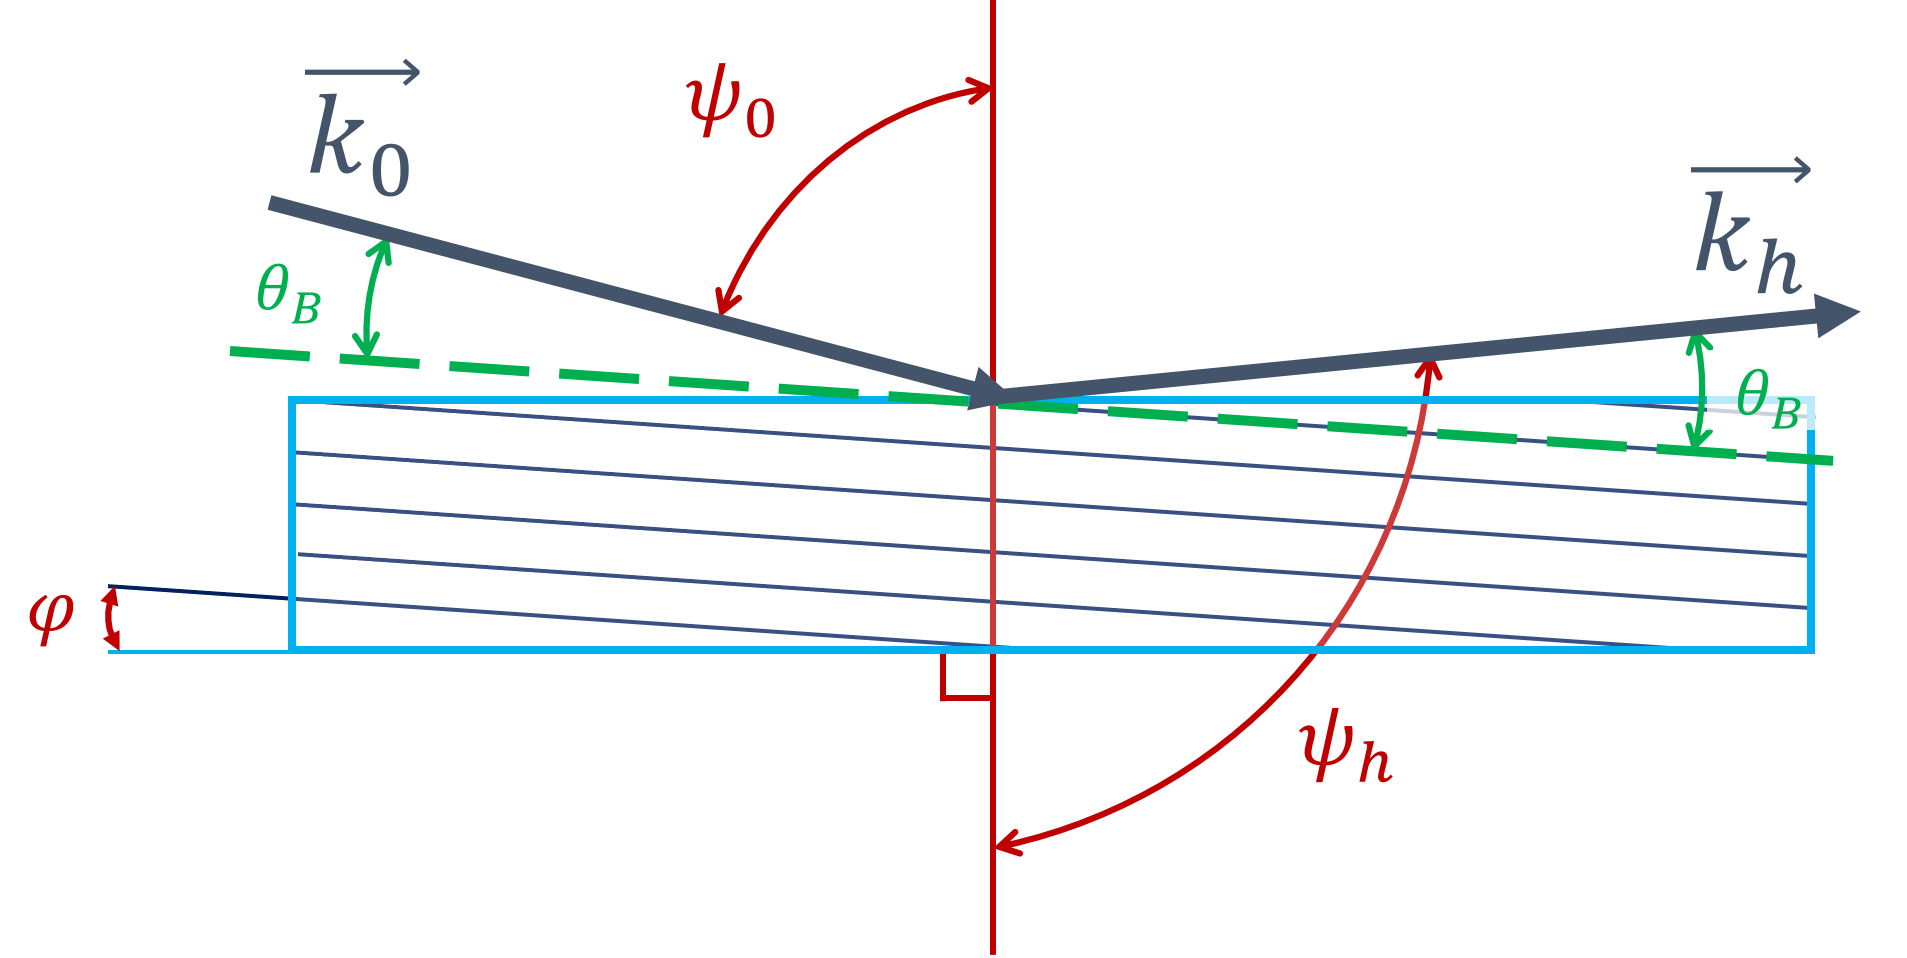
\includegraphics[width=0.45\textwidth]{images/assym2.png}\label{fig:f1}}
  \hfill
  \subfloat[$b << 1$, $\varphi$ < 0]{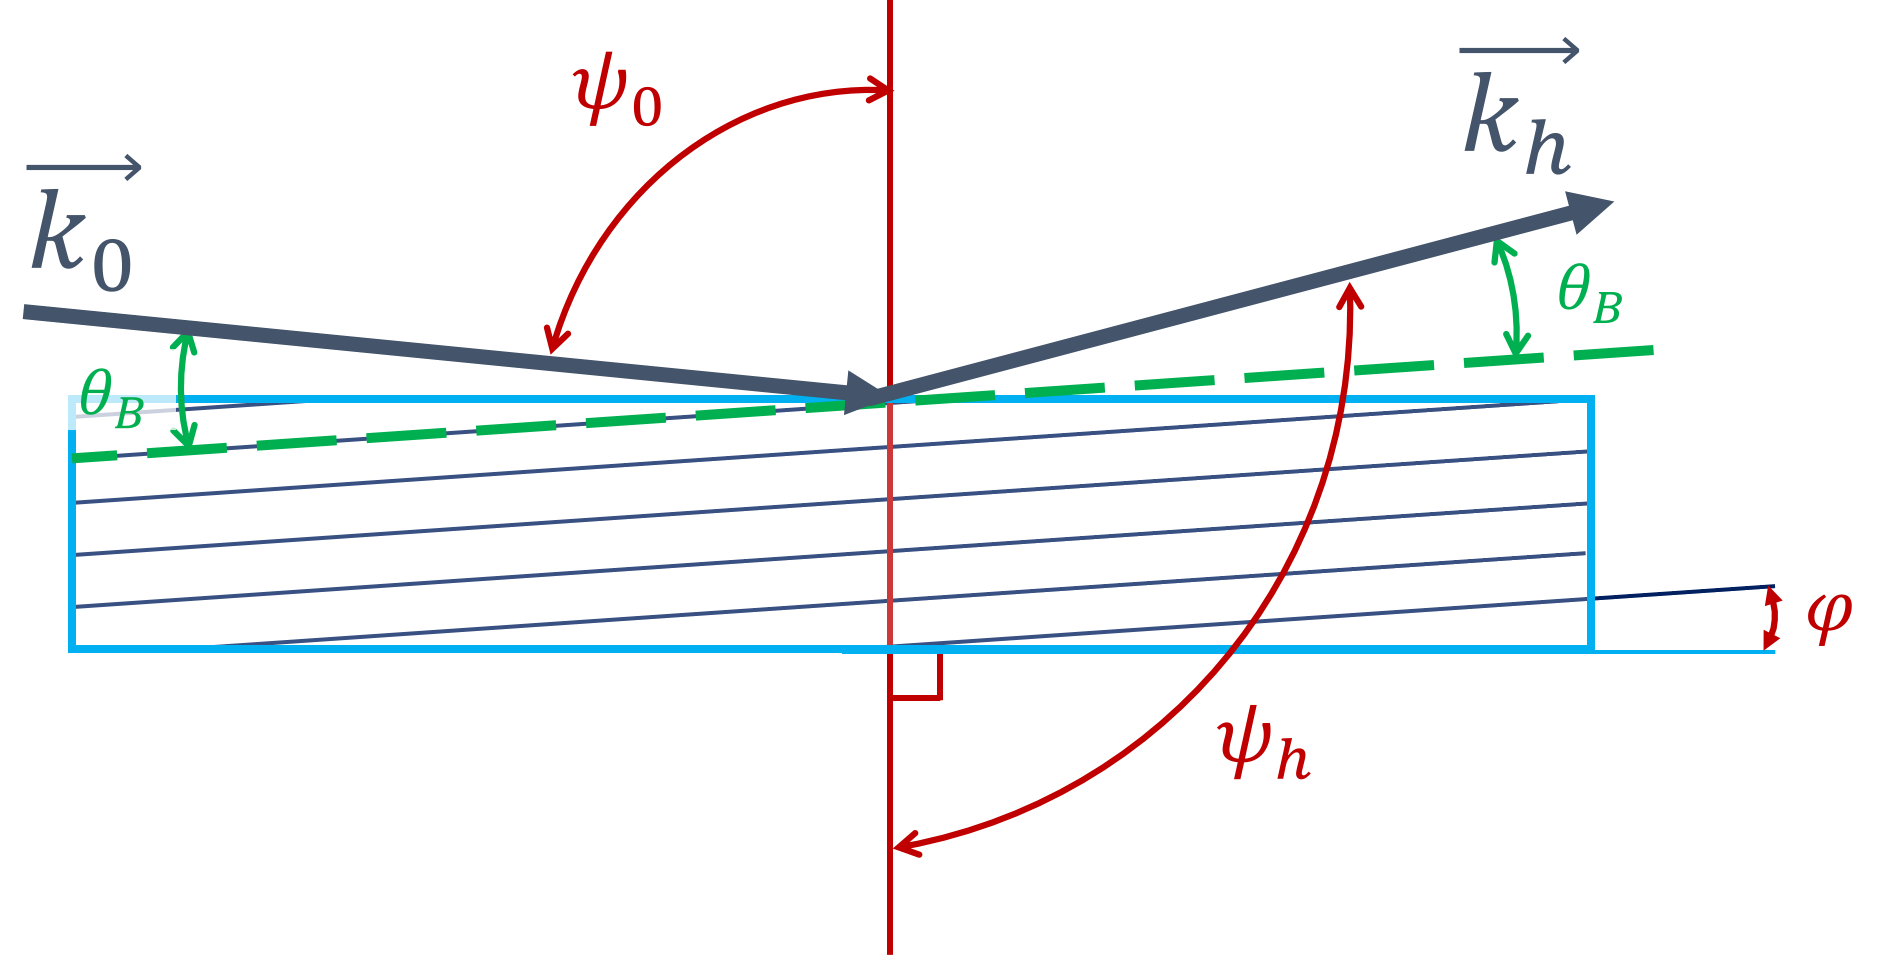
\includegraphics[width=0.45\textwidth]{images/assym1.png}\label{fig:f2}}
  \caption{Схема Брегговской дифракции для асимметричного отражения}
  \label{ris:assymetric_brag}
\end{figure}

Для того чтобы охарактеризовать степень асимметрии, введем коэффициент $b$:

\begin{equation}
  b = \frac {\gamma_0}{|\gamma_h|}
 \end{equation}
где, $\gamma_0 = cos \psi_0 = sin ( \varphi + \theta_B)$, $\gamma_h = cos \psi_h = sin ( \varphi - \theta_B)$,
$\varphi$ - угол между плоскостью отражения и поверхностью образца.


Весьма наглядной иллюстрацией являются собственные кривые отражения от Si(440) рассчитанные при
трех разных углах падения и соответсвенно имею разный коэффициент асимметрии. Угол
Брегга для такой плоскости отражения составляет $\theta_B = 21.68^o$, угол наклона поверхности
составляет $\varphi = 20^o 53^{'}$.

\begin{figure}[H]
\centering
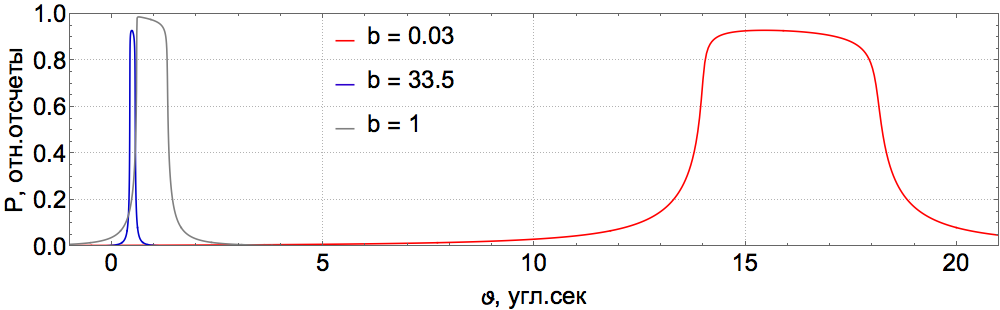
\includegraphics[width=0.99\textwidth]{images/rocking_curve_assym_3.png}
\caption{Кривые отражения 440 $MoK_{\alpha 1}$ от Si, полученные при разных углах падения(для разных b)}
\label{ris:rocking_curve_assym_3}
\end{figure}
Сдвиг центра кривой происходит из-за наличия преломления на величину 0.5 и 16.5 угловых секунд.

Варьируя угол между поверхностью кристалла и отражающей плоскостью (например, с помощью шлифовки),
можно существенно изменить ширину рентгеновского пучка (рисунок ~\ref{ris:assym_width_beam}).
\begin{figure}[H]
 \centering
 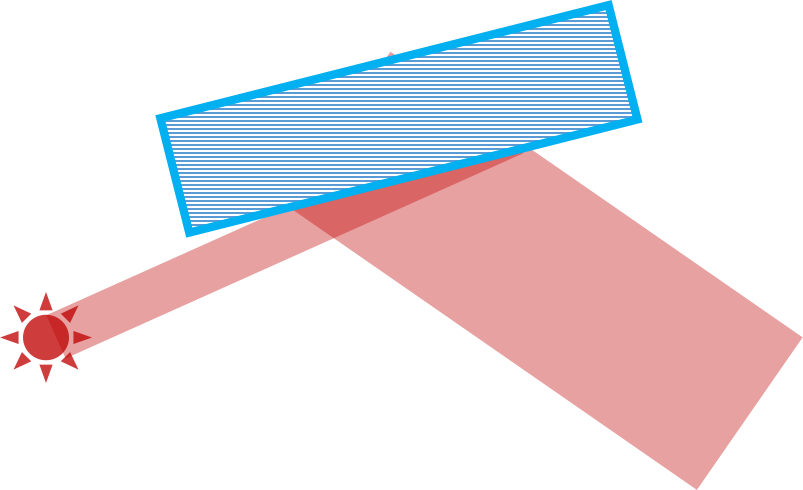
\includegraphics[width=0.4\textwidth]{images/assym_width_beam.png}
 \caption{Кристалл с асимметричным отражением по Бреггу}
 \label{ris:assym_width_beam}
\end{figure}

    \subsubsection{Рентгеновская поляризуемость в среде}
      
Вне кристалла, падающая волна описывается в виде совокупности плоских волн с волновым вектором  $\vec{k_0}$.
\begin{equation}
  \vec{E}_0(\vec{r},t) = E_0 e^{i(\vec{k}_0\vec{r}-\omega t)}
 \end{equation}

Падающая волна $vec{E}(\vec{r},t)_0$ порождает волновое поле внутри кристалла, которое характеризуется вектором
электромагнитной индукции $\vec{D}||\vec{E}$
\begin{equation}
 \vec{D}_0(\vec{r},t) = (1+\chi(\vec{r})) E_0 e^{i(\vec{k}_0\vec{r}-\omega t)} = A(r) e^{i(\vec{k}_0\vec{r}-\omega t)}
\end{equation}

где, $\chi$ - поляризуемость среды. Амплитуда волны $A(\vec{r})$ - не зависит
от времени, но зависит от координат, связано
это с тем что электроны колеблются под действие распространяющейся волны, и испускаемые ими
электромагнитные волны интерферируют между собой и с исходной волной. Устанавливается некоторое стабильное
электромагнитное поле с переодически изменяющейся в пространстве амплитудой. Периодичность эта должна быть
той же, что и периодичность решетки. Таким образом, в силу трехмерной периодичности $\chi(\vec{r}+\vec{h}) = \chi(\vec{r})$
, функцию $\chi(\vec{r})$ можно разложить в ряд Фурье и представить в виде

\begin{equation}
\chi(\vec{r}) = \sum_{h}\chi_h e^{i\vec{h}\vec{r}}
\end{equation}
Подробный вывод выражений для Фурье компонент $\chi_h$ представлен в (~\ref{sec:polarizability}), получим


\begin{equation}
\chi_h = -\frac{e^2 \lambda^2}{m \pi c^2} \frac{1}{V} \sum_{n} f_n \cdot e^{-2\pi i\vec{h}\cdot \vec{r}_n}
\end{equation}
где, $h$ - соответсвует какому - либо направлению вектора обратной решетки, для конкретных {hkl}.

На данном этапе мы не рассматриваем возможность распространение в кристалле большого количества
волн (многоголовой случай), а рассмотрим только два узла обратной решетки h - [000] и h - [hkl].
Тогда поляризуемость примет конечный вид

\begin{equation}
\chi(\vec{r}) = \chi_0 + \chi_h e^{i\vec{h}\vec{r}} + \chi_{-h} e^{-i\vec{h}\vec{r}}
\end{equation}

\textcolor{mygreen}{Если будет время, нарисовать распределение волнового поля для всех волн и их суммы}

    \subsubsection{Собственная кривая отражения (КДО)}
      
 \subsubsection{Коэффициент брегговского отражения от кристалла}
 Из системы уравнение Максвелла получим (~\ref{sec:wave_equation}) следующее волновое уравнение

\begin{equation}
 \Laplace \vec{E} - k_0^2 \vec{D} = \Laplace \vec{E} - k_0^2 (1+\chi)\vec{E} = 0
 \label{eq:wave_maxwel}
\end{equation}

как было упомянуто выше, в кристалле распространяются две волны
\begin{equation}
 \begin{cases}
   \vec{E}_0 = \vec{e}_0 E_0 e^{i\vec{q}_0\vec{r}}
   \\
   \vec{E}_h = \vec{e}_h E_h e^{i\vec{q}_h\vec{r}}
 \end{cases}
 \label{eq:E_0_E_h}
\end{equation}

где,

\begin{equation}
\vec{e}_0 \cdot \vec{e}_h = C
 \begin{cases}
   1, \quad \quad \quad \quad  \sigma    - \text{поляризация}\\
   \cos(2\theta_B), \quad   \pi - \text{поляризация}
 \end{cases}
\end{equation}

\begin{figure}[H]
  \centering
  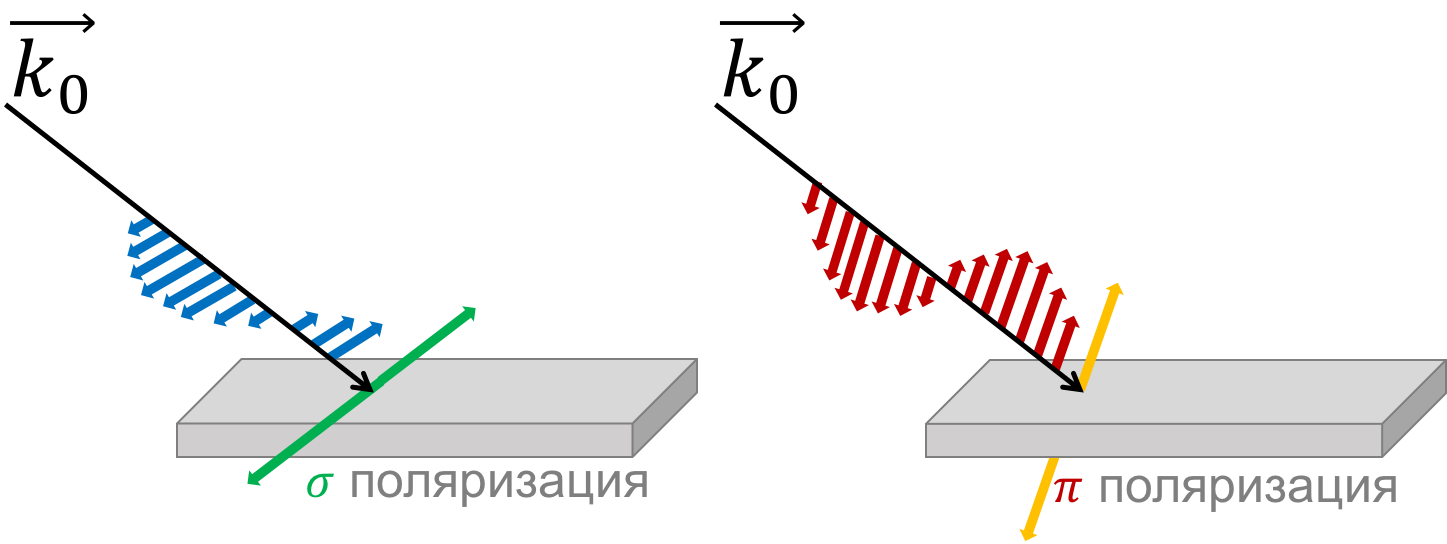
\includegraphics[width=0.7\textwidth]{images/polarize_E.png}
  \caption{ Колебание вектора напряженности электрического поля для разных типов линейной поляризации рентгеновского излучения}
  \label{ris:polarize_E}
\end{figure}

Подставим  ~\ref{eq:E_0_E_h} в уравнение ~\ref{eq:wave_maxwel} и получим
систему динамических уравнений
\begin{equation}
 \begin{cases}
   \delta_0 E_0 - C\chi_{-h}E_h=0
   \\
   \delta_h E_h - C\chi_{h}E_0=0
 \end{cases}
\end{equation}
где,
\begin{equation}
   \delta_{(0,h)} = \frac{q_{(0,h)}^2}{k_0^2}-1-\chi_0
\end{equation}

Прировняем детерминант системы к 0, получим дисперсионное уравнение

\begin{equation}
   \delta_0 \delta_h -C^2 \chi_h \chi_{-h} = 0
\end{equation}

Воспользуемся равенством тангенциальных компонент волнового вектора при переходе между средами (\ref{eq:k_h_squred}, \ref{eq:k_0_squred}),
необходимо отметить $k_h == q_h$ - т.к при выходе излучения из среды происходит лишь преломление, суммарная интенсивность останется прежней.
\begin{equation}
 \begin{cases}
   \delta_0 = \frac{q_0^2 - k_0^2}{k_0^2} - chi_0 = 2\varepsilon\gamma_0 - \chi_0
   \\
   \delta_h = \frac{q_h^2 - k_0^2}{k_0^2} - chi_0 = 2\varepsilon\gamma_h - \alpha \chi_0
 \end{cases}
\end{equation}
где $\alpha$ соответствует выражению (\ref{eq:alpha}). Дисперсионное уравнение с учетом граничных условий примет вид

\begin{equation}
   (2\varepsilon \gamma_0 - \chi_0)(2\varepsilon \gamma_h - \alpha - \chi_0) - C^2 \chi_h\chi_{-h} = 0
\end{equation}

Решив уравнение относительно параметра аккомодации $\varepsilon$ получим два корня

\begin{equation}
   \varepsilon_{1,2} = \frac{1}{4\gamma_0} \left( \chi_0 (1-b) - b\alpha \pm \left( [\chi_0(1+b)+b\alpha]^2 - 4bC^2 \cdot \chi_{h}\chi_{-h} \right)^{1/2} \right)
\end{equation}
где b - соответсвует (\ref{eq:koef_b}),  а произведение коэффициентов поляризуемости
 $$\chi_{h} \cdot \chi_{-h} = Re(\chi_{h})^2-Im(\chi_{h})^2 - 2i \quad Re(\chi_{h}) \cdot Im(\chi_{h})$$

Наличие двух решений говорит о том, что в кристалле имеется две проходящие и две дифрагированные волны, но
анализ полученного решения $ \varepsilon_{1,2}$ показывает что один корень имеет положительную мнимую часть, а второй
отрицательную. Мнимая часть отвечает за поглощение и в случае отрицательно корня волна распространяясь
вглубь кристалла экспоненциально затухает. Поэтому будем выбирать всегда корень с отрицательной мнимой частью
$Im(\varepsilon)>0$.

Амплитудный коэффициент отражение
\begin{equation}
    R = \frac{E_0}{E_h} = \frac{\delta_0}{C\chi_{-h}} = \frac{2\varepsilon\gamma_0-\chi_0}{C\chi_{-h}}
\end{equation}

Кривая диффракционного отражения (КДО) \cite{Bushuev_Oreshko_2002}
\begin{equation}
    \label{eq:KDO_self}
    P (\vartheta) =  |\frac{\gamma_h}{\gamma_0} \cdot R|^2
\end{equation}

    % \subsubsection{Нарушенный слой}
      % \subsubsection{Нарушенный слой}

  \subsection{Пьезоэлектрический эффект}
    \label{sec:piezo_theor}
В материалах обладающих пьезоэлектрическими свойствами существует
линейная связь между механическим напряжением и электрической поляризаций
(прямой пьезоэлектрический эффект) или между механической деформацией
и приложенным электрическим полем (обратный пьезоэлектрический эффект).

\begin{figure}[H]
  \centering
  \subfloat[Деформация кристаллической структуры вызывает появление
  разности электрических потенциалов на гранях кристалла (прямой пьезоэлектрический эффект)
  ]{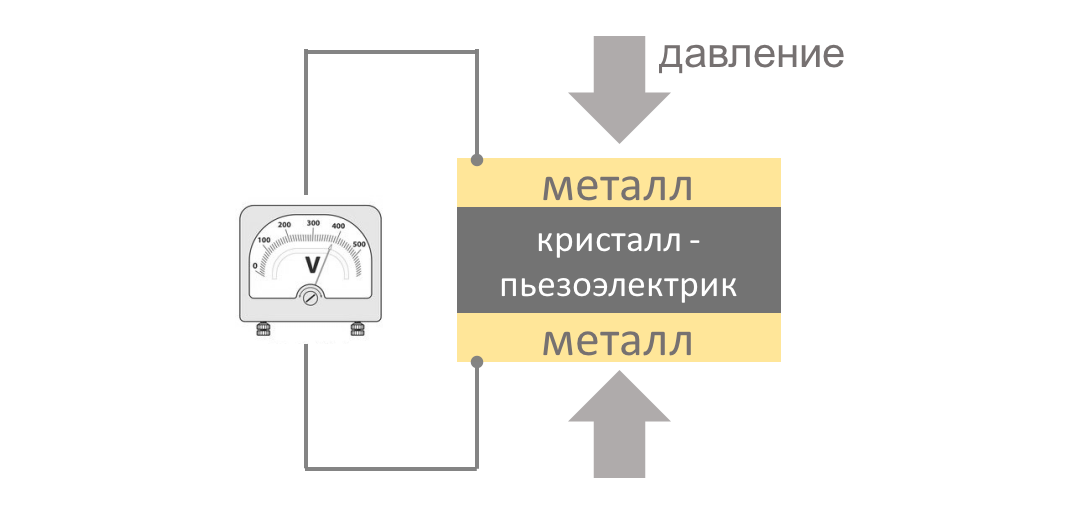
\includegraphics[width=0.4\textwidth]{images/piezo_ther_1.png}}
  \hfill
  \subfloat[Внешнее электрическое поле вызывает деформацию кристалла
  (обратный пьезоэлектрический эффект)]{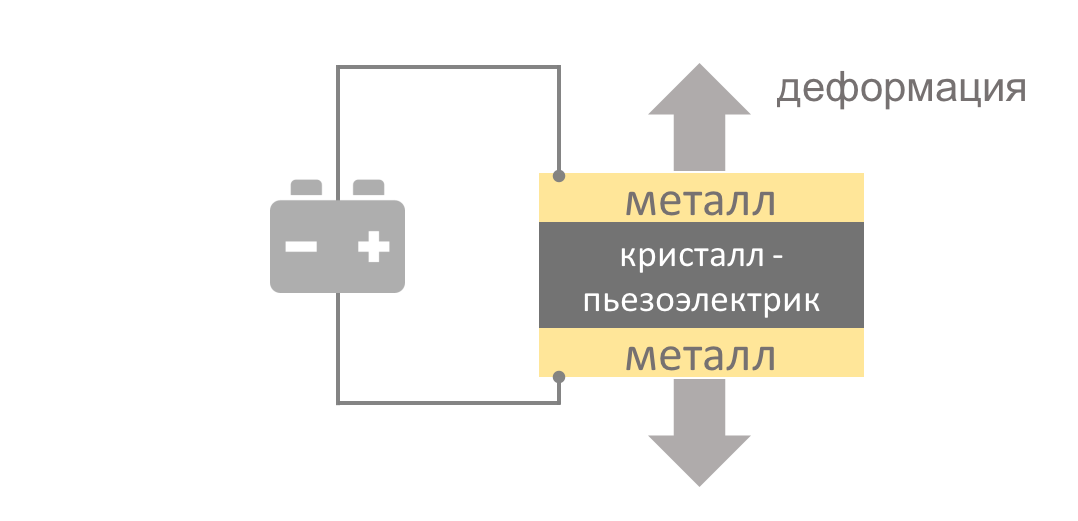
\includegraphics[width=0.45\textwidth]{images/piezo_ther_2.png}}
  \caption{Свойство пьезоэлектрического кристалла в его простейшем виде}
  \label{ris:piezo_is}
\end{figure}

Согласно определению обратного пьезоэлектрического эффекта,
приложенное внешнее электрическое поле $\vec{E}$ является причиной возникновения
в кристаллическом материале деформаций $r_i$. Вектор деформаций пропорционален
величине приложенного напряжения и зависит от пьезоэлектрических свойств материала
в данном направлении $d$. Модуль пьезоэлектрических деформаций $d$ является
матричной 3х6 \cite{kedi_1949,Newnham_2005}.


\begin{equation}
  r_j = d_{ij}E_i
  \label{eq:piezomodule}
\end{equation}
где $i = (1,2,3) = (x,y,z)$, $j = (1,2,3,4,5,6)$, $E_i$ - компонента напряженности электрического поля.

Исходя из уравнения (\ref{eq:piezomodule}) можно судить о том, что поле приложенное в каком-либо из
направлений может вызывать деформацию кристалла в любом направлении с коэффициентом пропорциональности $d_{ij}$.

Компоненты деформации  $r_1$, $r_2$ ...$r_6$ можно также обозначать  через $x_x$, $y_y$, $z_z$,
$y_z$, $z_x$ и $x_y$ (обозначения Кирхгофа)  \cite{kedi_1949}.

Они связаны со смещением следующим образом:
\begin{figure}[H]
  \centering
  \subfloat[]{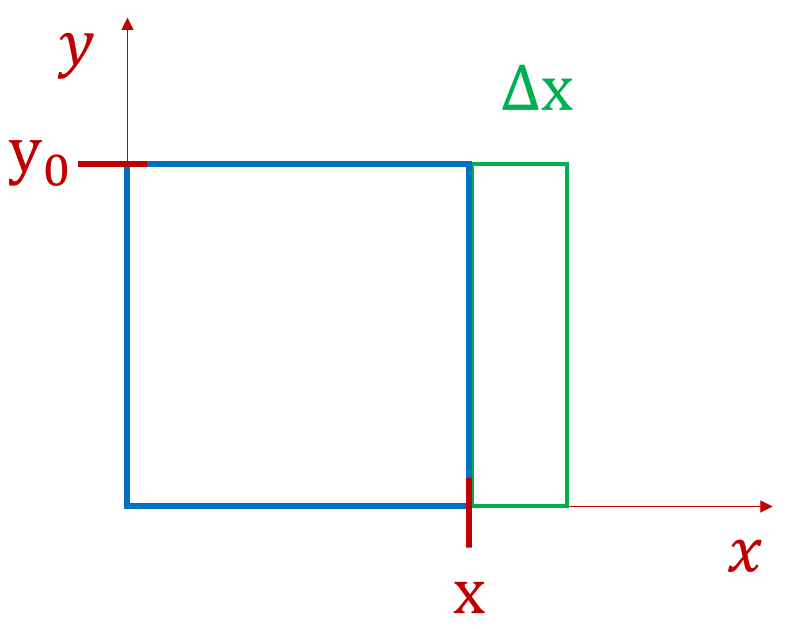
\includegraphics[width=0.45\textwidth]{images/x_x_2d.png}}
  \hfill
  \subfloat[]{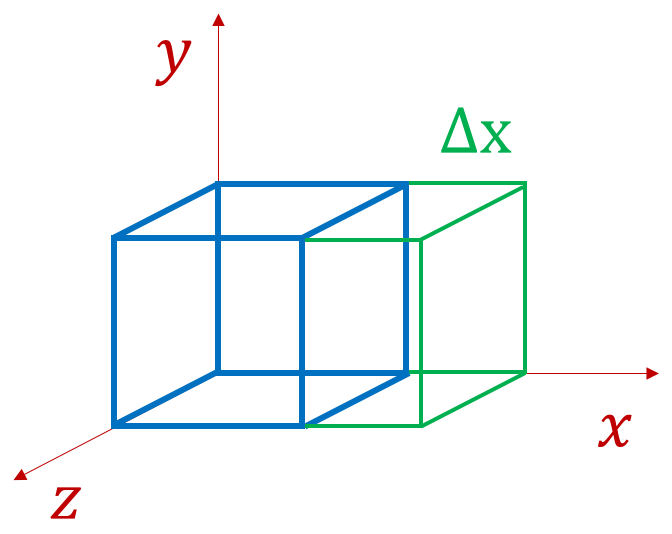
\includegraphics[width=0.45\textwidth]{images/x_x_3d.png}}
  \caption{К объяснению деформации растяжения и сжатия. $r_1= x_x = \frac{\Delta x}{x_0} $}
  \label{ris:}
\end{figure}

\begin{figure}[H]
  \centering
  \subfloat[на плоскости]{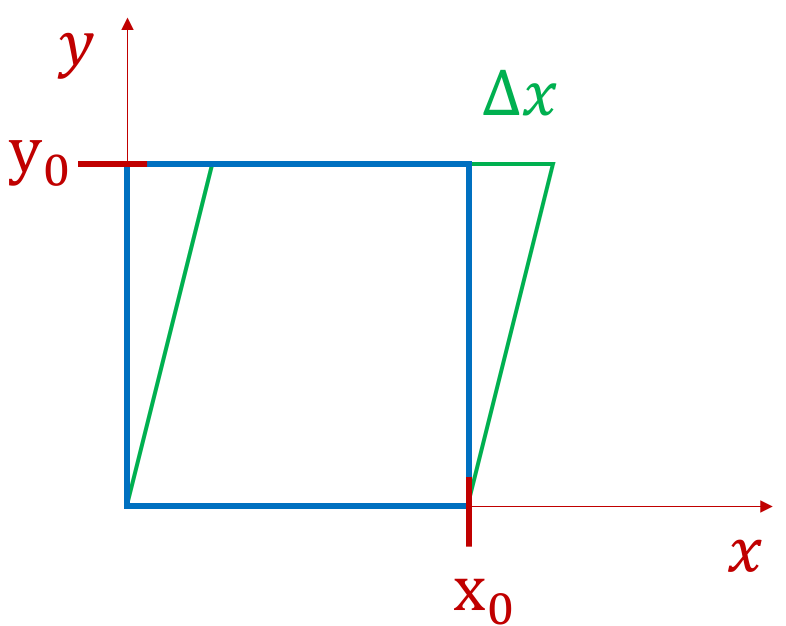
\includegraphics[width=0.45\textwidth]{images/x_y_2d.png}}
  \hfill
  \subfloat[в объеме]{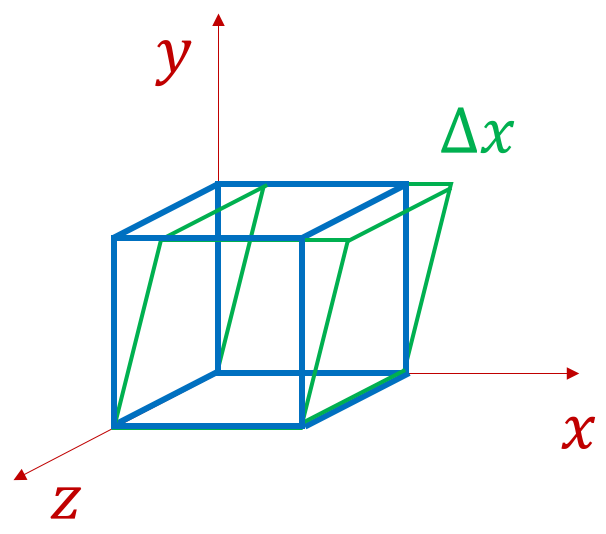
\includegraphics[width=0.45\textwidth]{images/x_y_3d.png}}
  \caption{К объяснению деформации сдвига. $r_6= x_y = \frac{\Delta x}{y_0} $}
  \label{ris:x_y_2d}
\end{figure}

Поясняя рисунок \ref{ris:x_y_2d}, в случае деформации сдвига обозначают
компоненты векторов в плоскости которых происходит деформация. Если $x_y$ и $y_x$
налагаются одновременно, такую деформацию можно представить в виде одного из
смещений с учетом поворота всего образца, так если например $x_y = y_x$, произойдет
просто удвоение одной из компонент (рисунок \ref{ris:2x_y_1}). С математической
точки зрения отождествление компонент $x_y$ с $y_x$ уменьшает число компонент
общего тенора деформаций.

\begin{figure}[H]
  \centering
  \subfloat[на плоскости]{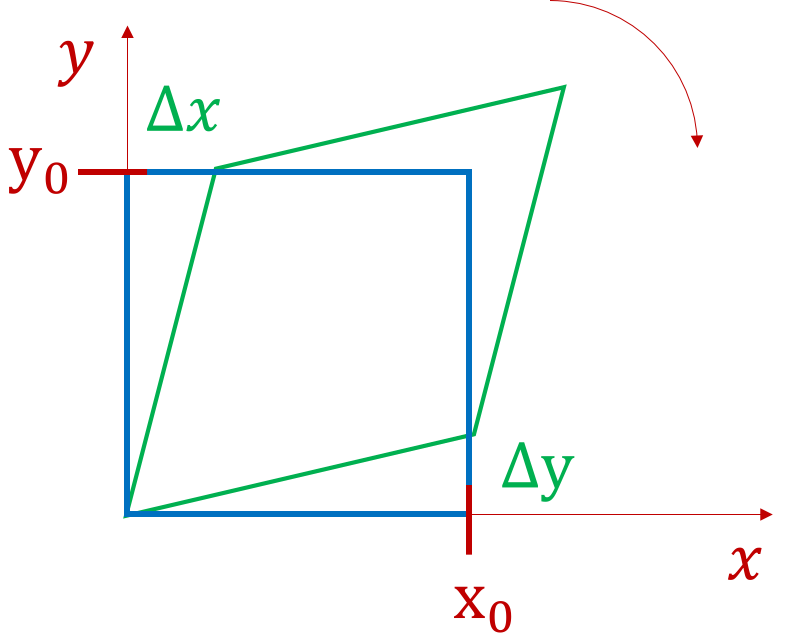
\includegraphics[width=0.45\textwidth]{images/2x_y_1.png}}
  \hfill
  \subfloat[в объеме]{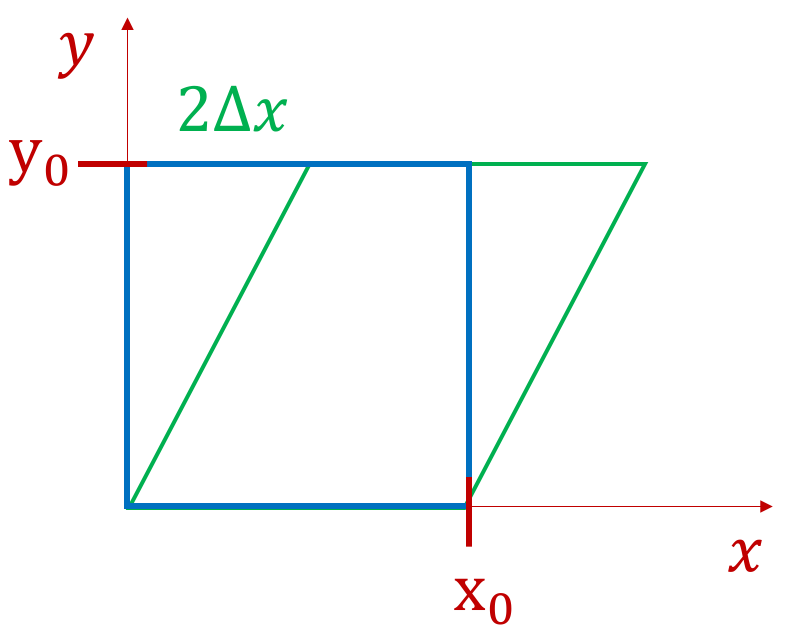
\includegraphics[width=0.45\textwidth]{images/2x_y_2.png}}
  \caption{Отождествление компонент деформации $x_y$ с $y_x$ }
  \label{ris:2x_y_1}
\end{figure}

В развернутой форме выражение (\ref{eq:piezomodule}) выглядит как

\begin{equation}
  \begin{pmatrix}
  r_1 \\
  r_2 \\
  r_3 \\
  r_4 \\
  r_5 \\
  r_6
  \end{pmatrix}
   = \begin{pmatrix}
  d_{11} & d_{21}  & d_{31} \\
  d_{12} & d_{22}  & d_{32} \\
  d_{13} & d_{23}  & d_{33} \\
  d_{14} & d_{24}  & d_{34} \\
  d_{15} & d_{25}  & d_{35} \\
  d_{16} & d_{26}  & d_{36}
  \end{pmatrix}
  \begin{pmatrix}
  E_1 \\
  E_2 \\
  E_3
  \end{pmatrix}
  \label{eq:piezomodule_matrica}
\end{equation}

В общем случае все 18 пьезомодулей не зависимы друг от друга. Однако
под действием операции симметрии кристалл должен должен полностью совместиться с
самим собой и это касается не только его строения, но и любого физического свойства.
Исходя из принципа Неймана \cite{Shaskolska_1984}, физические свойства, в частном случае
пьезоэффект, по кристаллографически эквивалентным направлениям должны быть одинаковыми.
Таким образом, пьезоэлектрический эффект может возникнуть в кристаллах, лишенных центра
симметрии. В 11 классах точеной группы симметрии из 32 нет полярных направлений,
а значит в кристаллах этих классов не может возникать пьезоэффект. Для остальных
классов, некоторые пьезомодули могут обратиться в нуль из-за наличия симметрии.
Другими словами, чем выше симметрия, тем меньше число независимых пьезомодулей.
Матрицы пьезомодулей $d$, для кристаллов используемых в расчетах и экспериментах ниже,
  приведены в разделе (\ref{sec:piezo_matrix}).


% ---------------------section 2 -----------------------
\newpage
\section{Оборудование и методы}
  \subsection{Оборудование. Трехкристальный рентгеновский спектрометр}
    Апробация результатов расчетов производилась на лабораторном источнике
рентгеновского излучения (рис. \ref{ris:trs}). Трехкристальный рентгеновский
спектрометр (ТРС) представляет из себя источник с молибденовым анодом, который является
неподвижным в процессе сканирования. Рентгеновские лучи от источника падают на
 кристалл монохроматор, где происходит выделение спектрального дублета. Щелевое
 устройство № 1 отделяет спектральную составляющую, котороя затем отражается от
 исследуемого кристалла.

\begin{figure}[H]
  \centering
  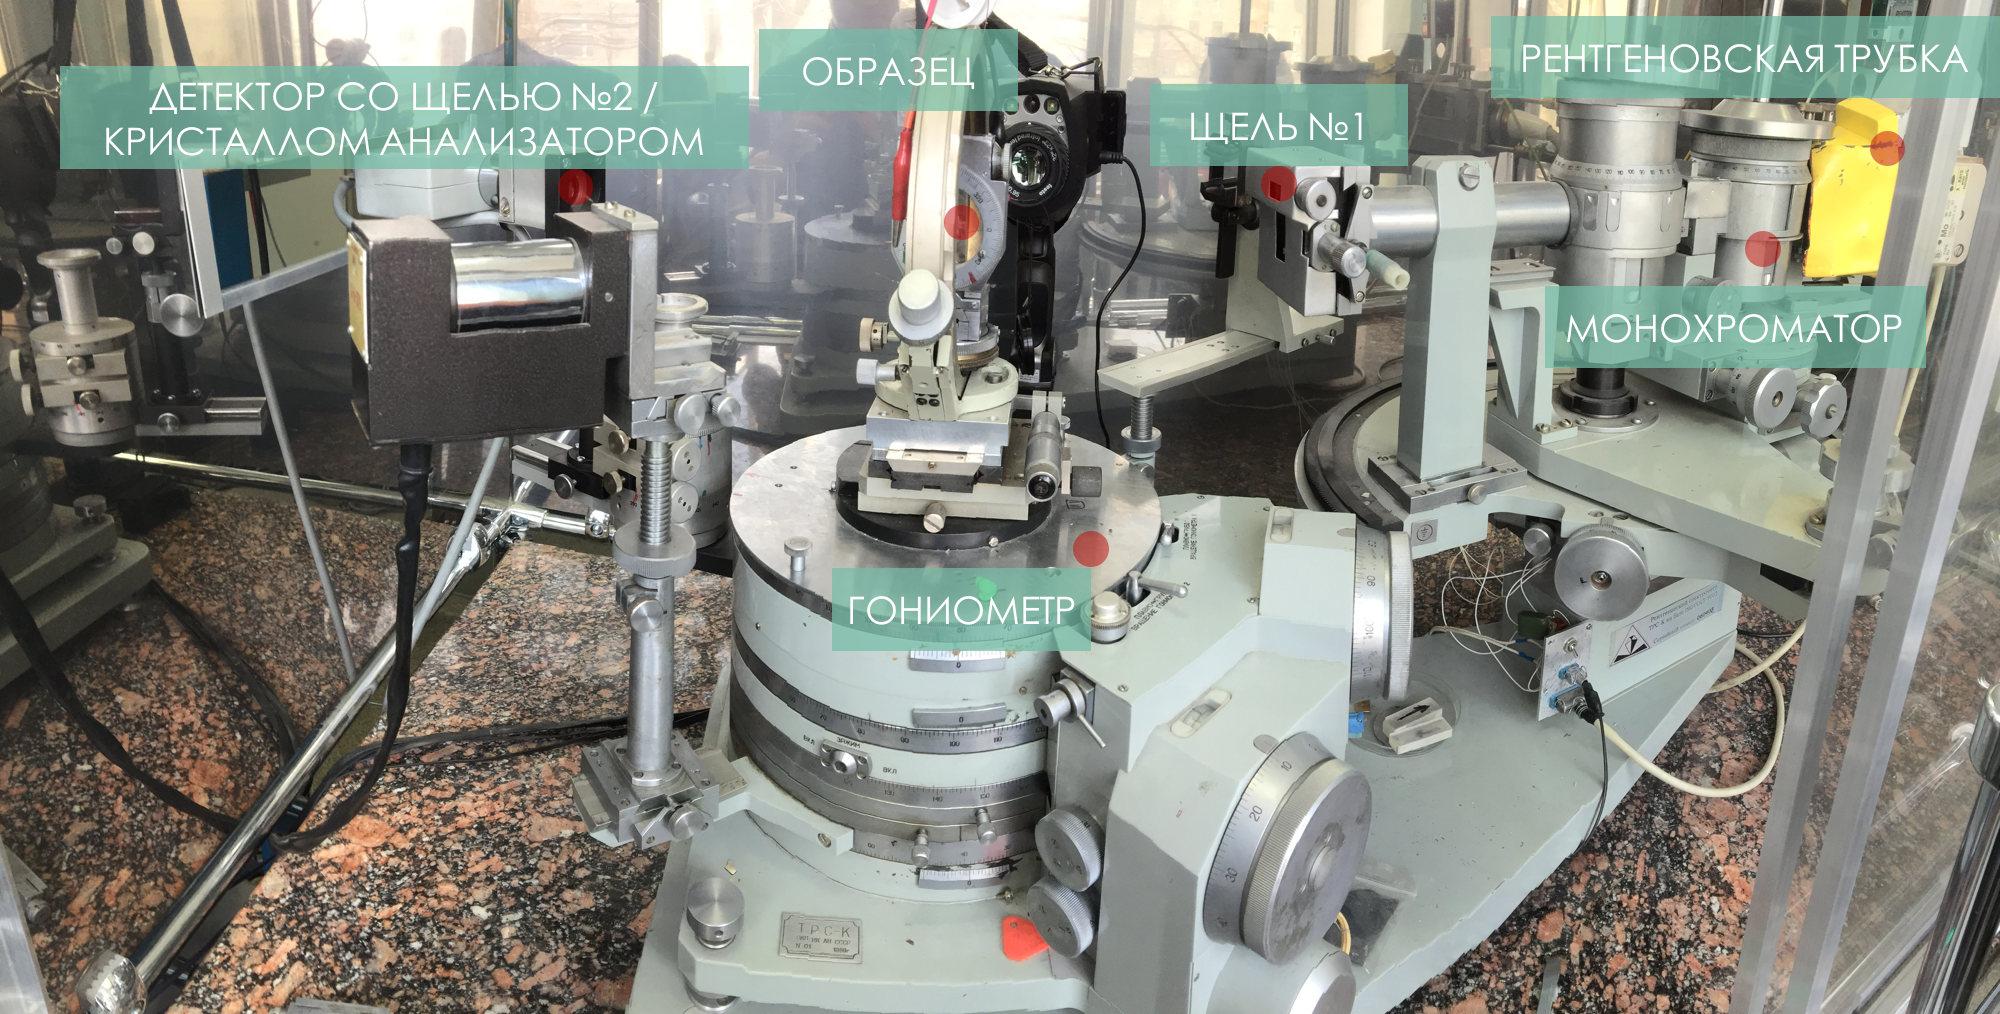
\includegraphics[width=1\textwidth]{images/trs.png}
  \caption{ Трехкристальный рентгеновский спектрометр. Лаборатория рентгеновских
  методов анализа и синхратронного излучения, ФНИЦ "Кристаллография и фотоника"}
  \label{ris:trs}
\end{figure}

ТРС имеет возможность работать в режиме двухкристального эксперимента,
в таком случае непосредственно перед детектором устанавливается щелевое устройство
№ 2, все прошедшие лучи фиксируются детектором.

Для случая необходимости получения трехкристальных кривых дифракционного отражения,
на место перед детектором устанавливается кристалл анализатор, отраженный от анализатора луч
фиксируется детектором.

  \subsection{Исследуемые образцы}
        \label{sec:piezo_matrix}

  \subsubsection*{ Кристалл Si }
  Для проведения экспериментов, необходимых для апробации разрабатываемых алгоритмов,
  был использован монокристалл кремния (Si). Данный
  кристалл характеризуется идеальной кривой собственного отражения, поэтому
  был использован в качестве модельного образца. Решетка Si имеет кубическую симметрию
  с параметрами элементарной ячейки  $a = b = c = 5.4310 \angstrom$.

  \subsubsection*{ Кристалл LGT }
  Кристаллы семейства лантан-галлиевого силиката ($La_3Ga_5SiO_{14}$ - LGS и $La_3Ga_{5.5}Ta_{0.5}O_{14}$ - LGT)
  обладают пьезоэлектрическими свойствами со стабильной температурной зависимостью
  даже при высоких температурах. Пьзоэлектрический модуль $d_{11}$ остается
  постоянным в диапазоне температур до $600^o$С (изменение не более 5 $\%$ \cite{LGS58}).
  В таких кристаллах отсутствует фазовый переход вплоть до температур плавления \cite{LGS57},
   а также не имеется пироэлектрического эффекта.

  LGT кристалл имеет точечную группу симметрии $32$ и гексагональную сингонию.
  Матрица пьезоэлектрических модулей выглядит следующим образом:
  \begin{equation}
    \begin{pmatrix}
    d_{11} & -d_{11} & 0 & d_{14} & 0 & 0 \\
    0 & 0 & 0 & 0 & -d_{14} & 2d_{11} \\
    0 & 0 & 0 & 0 & 0 & 0
    \end{pmatrix}.
    \label{eq:piezomodule_lgt_matrica}
  \end{equation}
  Параметры ячейки: $a = b = 8.228 \angstrom$, $c = 5.124 \angstrom$ \cite{marchenkov2014}.
  %
  % \subsection*{ Кристалл $TeO_2$ }
  % ...
  % \subsection*{ Кристалл $Li_2B_4O_7$ }
  % ...

  \subsection{Алгоритмы расчетов и методики измерений}
    Стоит отметить, что представление параметров рентгеновского пучка
 в виде двумерных спектрально-угловых карт (рис. \ref{ris:source_distrubition})
 будет использовано далее во всей работе. Это позволяет не только наглядно отслеживать
характеристики излучения после прохождения каждого элемента рентгенооптической
схемы, но и проводить моделирование как для любых типов источников, так
и для разных элементов схемы. Такой подход основывается на представлении, впервые предложенном
ДюМондом \cite{Dumond1937}.

    \subsubsection{Функция источника}
      \label{sec:source_section}
Аппаратная функция дифрактометра определяется спектральной и угловой
составляющей. Излучение рентгеновской трубки представляет из себя комбинацию
 непрерывного тормозного спектра \cite{blohin1957} и характеристического, спектральная часть
 которого достаточно хорошо описывается суперпозицией двух функций Лоренца, взятых с
 весовыми коэффициентами 2:1 (\ref{eq:source_spectral}):

 \begin{equation} \label{eq:source_spectral}
   g_{\lambda} (\lambda) = \frac{2\pi}{3}  \left \{ \frac{\delta\lambda_1}{(\lambda - \lambda_1)^2+
   (\delta \lambda_1)^2} + \frac{1}{2} \frac{\delta\lambda_2}{(\lambda-\lambda_1)^2+(\delta\lambda_1)^2} \right \},
  \end{equation}
\noindent
где $\frac{2\pi}{3}$ - нормировочный коэффициент.

  Плотность распределения количества фотонов электромагнитного излучения в зависимости от угла
  отстройки относительно прямолинейного распределения задается функцией Гаусса (\ref{eq:source_angle}):
\begin{equation} \label{eq:source_angle}
  g_{\vartheta} (\vartheta) = \frac{1}{\sigma \sqrt{ 2\pi}} exp  ( -\frac{\vartheta^2}{2\sigma^2} ),
 \end{equation}
\noindent
где $\sigma$ - параметр, который характеризует ширину углового распределения на половине высоты.

\begin{figure}[H]
  \centering
  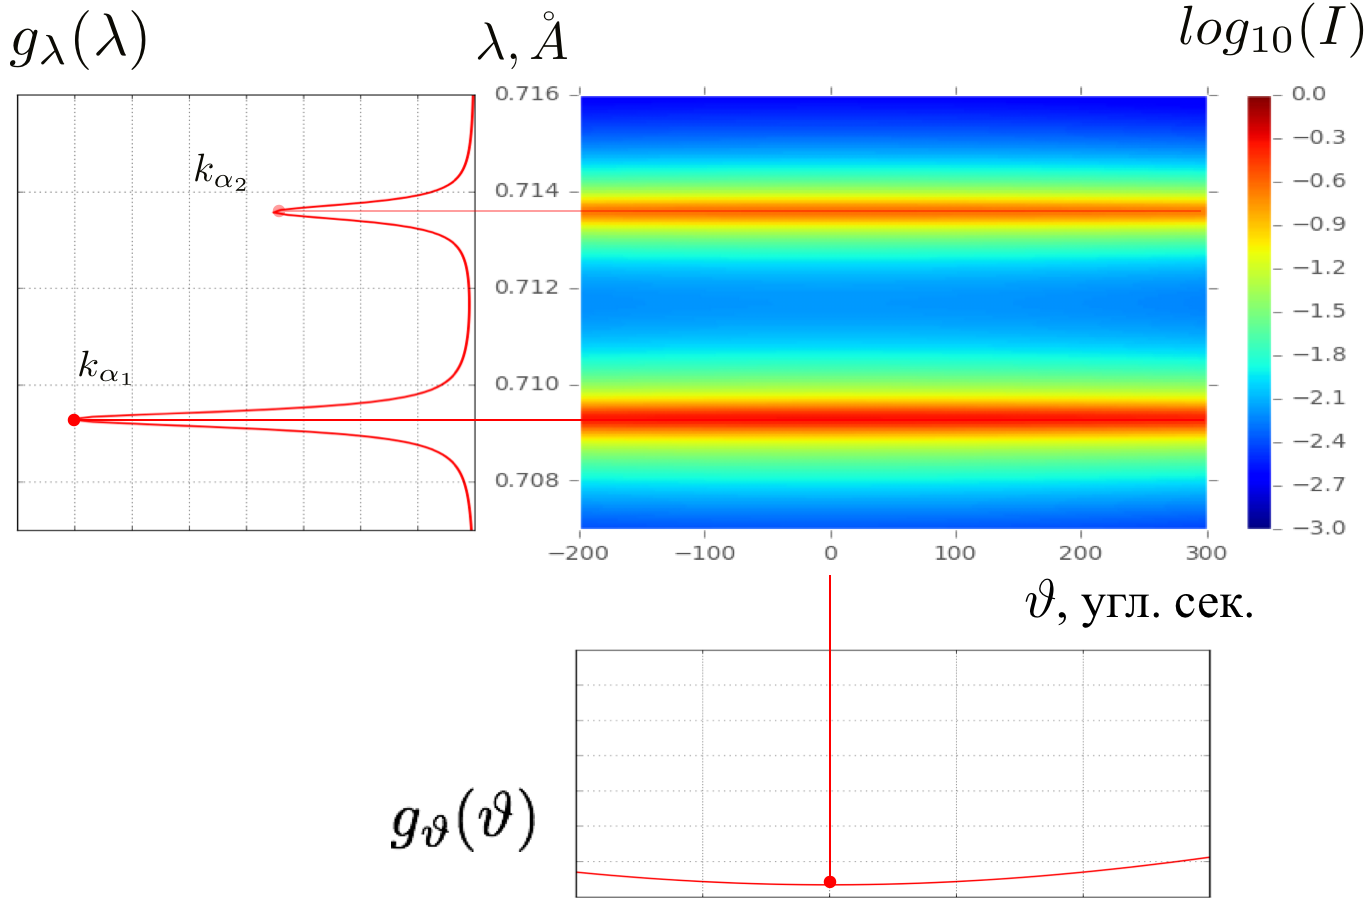
\includegraphics[width=0.6\textwidth]{images/source_distrubition.png}
  \caption{Спектрально – угловое распределение лабораторного источника рентгеновского
   излучения с молибденовым анодом, полуширина гауссова распределения составляет $\sigma = 600$ угл. сек. }
  \label{ris:source_distrubition}
\end{figure}

    \subsubsection{Функция щелевых коллиматоров}
      \label{sec:slits_section}
Другой составляющей аппаратной функции является функция углового распределения излучения в
экспериментальной схеме, определяемая геометрическими особенностями (размерами щелевых
коллиматоров и длинами оптических путей). Рассмотрим преобразование пучка рентгеновского
 излучения проходящего через систему щелевых коллиматоров.
\begin{figure}[H]
  \centering
  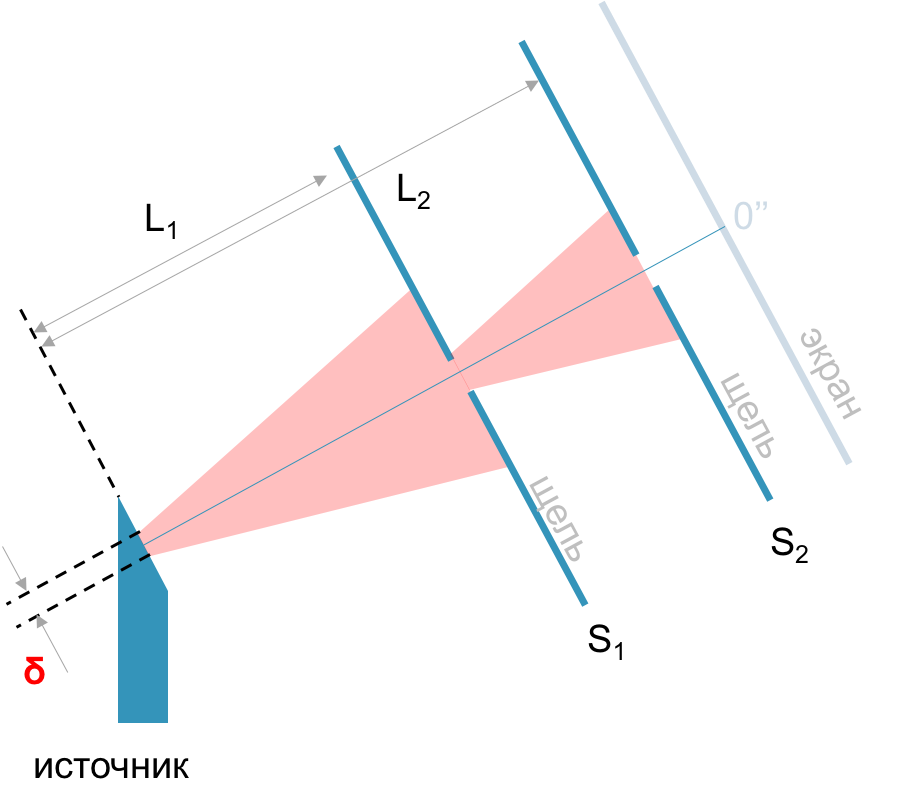
\includegraphics[width=0.6\textwidth]{images/for_slits.png}
  \caption{Схематичное изображение распространение рентгеновского пучка в
  системе с протяженным источником и двумя щелевыми коллиматорами}
  \label{ris:for_slits}
\end{figure}

На начальном этапе рассматривалась модель точечного источника излучения
 (протяженность источника $\delta = 0$).
В таком случае, интенсивность проходящего излучения будет определятся
одним щелевым коллиматором, которое является более узким из двух при пересчете в угловые
координаты. Например, для фиксированных расстояний между элементами $L_1 = 570$ мм, $L_2 = 1005$ мм,
 в случае одинаковых линейных размеров щелей и точечного
источника, интенсивность будет определяться более удаленным щелевым коллиматором, и
распределение интенсивности принимает вид представленный на рис. \ref{ris:sourc_map_a}. Если источник является
протяженным ($\delta \neq 0$), то угловое распределение интенсивности принимает более сложный вид,
 как показано на рис. \ref{ris:sourc_map_b}.


\begin{figure}[H]
  \centering
  \subfloat[]{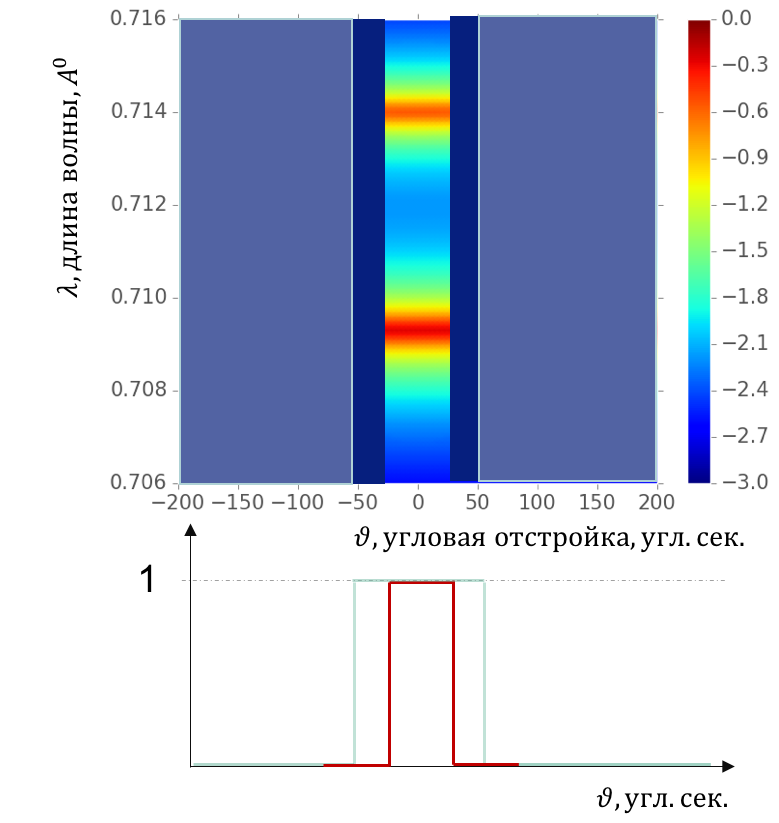
\includegraphics[width=0.5\textwidth]{images/point_sourc_map.png}\label{ris:sourc_map_a}}
  \hfill
  \subfloat[]{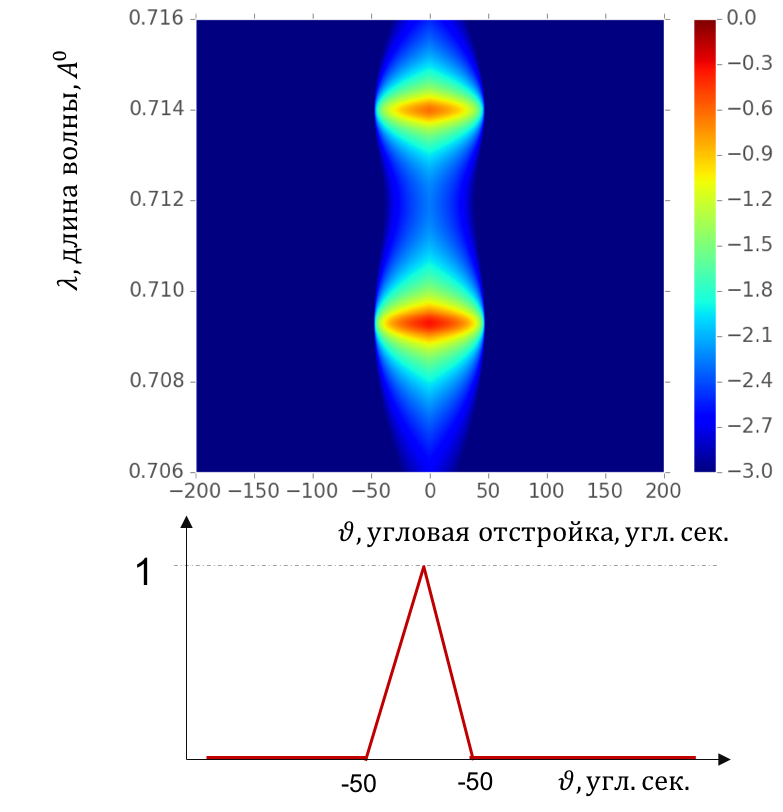
\includegraphics[width=0.5\textwidth]{images/wide_sourc_map.png}\label{ris:sourc_map_b}}
  \caption{Спектрально-угловое распределение излучения в системе двух щелей для различных типов источника: точечного (a)
  и протяженного ($\delta = 0.2$ мм) (b), $MoK_{\alpha}$ - излучение}
  \label{ris:sourc_map}
\end{figure}

Необходимо отметить, что для описания дифракционного эксперимента имеет значение именно
спектрально-угловое распределение излучения, т.е. количество и энергия квантов, падающих под тем
или иным углом на кристалл. Данное распределение определяется соотношение площадей параллелограммов,
угол между боковой стороной и основанием которых соответсвует углу распространения излучения
(рис. \ref{ris:how_many_quants_use_parallelogr}).

\begin{figure}[H]
  \centering
  \subfloat[]{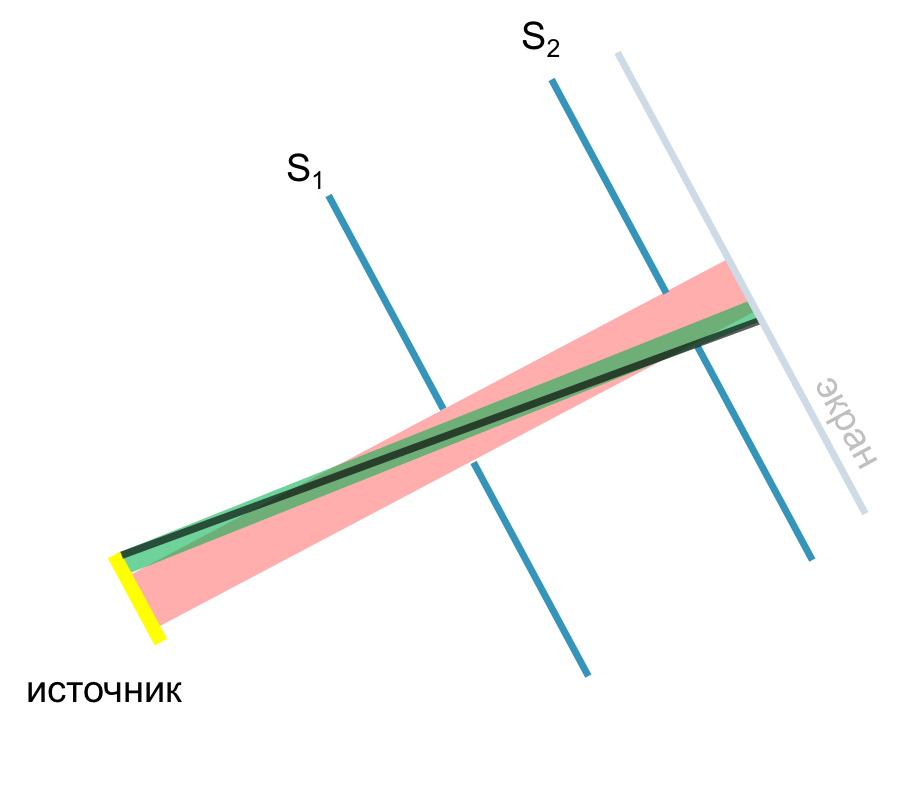
\includegraphics[width=0.45\textwidth]{images/how_many_quants_use_parallelogr_1.png}}
  \hfill
  \subfloat[]{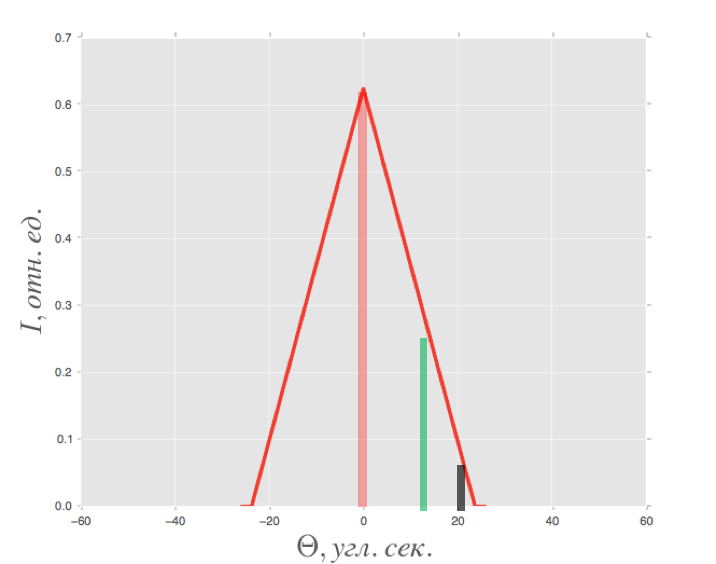
\includegraphics[width=0.45\textwidth]{images/how_many_quants_use_parallelogr_2.png}}
  \caption{Схематичное представление углового распределения излучения после
  прохождения системы щелевых коллиматоров. Пропускная способность системы
  щелей в определенном угловом направлении соответствующего параллелограмма (a).
   Интенсивность на экране, установленном после системы щелей для
   протяженности источника $\delta = 0.2$ мм (b)}
  \label{ris:how_many_quants_use_parallelogr}
\end{figure}
Более подробный расчет $g_S(\vartheta)$ представлен в Приложении 3.
На рис. \ref{ris:calc_slits_ability_res} представлены результаты расчета пропускной способности
системы двух щелей для некоторых параметров ренгенооптической схемы в приближении
 точечного источника ($\delta = 0$), в сравнении с протяженным ($\delta \neq 0$).

\begin{figure}[H]
 \centering
 \subfloat[]{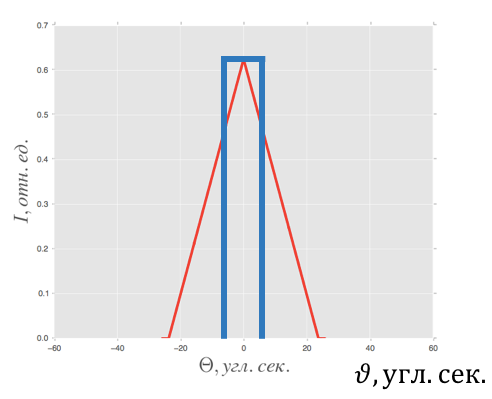
\includegraphics[height=6em]{images/calc_slits_ability_res_1.png}}
 \hfill
 \subfloat[]{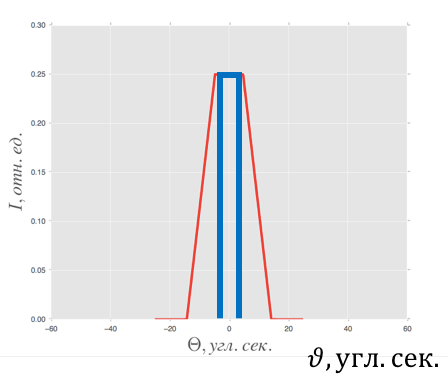
\includegraphics[height=6em]{images/calc_slits_ability_res_2.png}}
 \hfill
 \subfloat[]{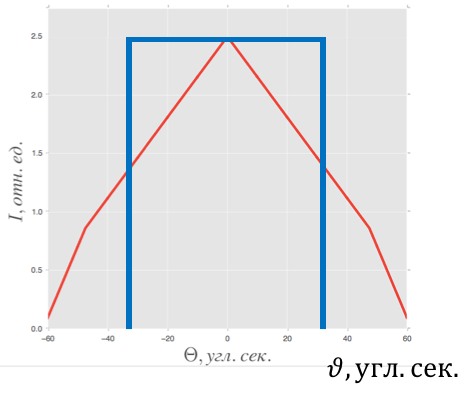
\includegraphics[height=6em]{images/calc_slits_ability_res_3.png}}
 \hfill
 \subfloat[]{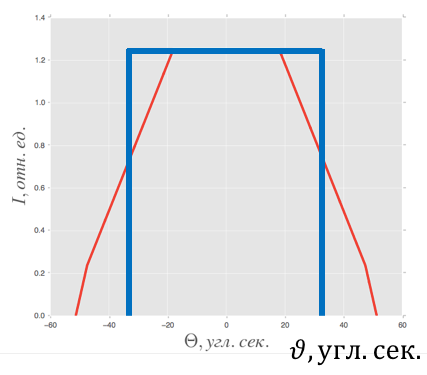
\includegraphics[height=6em]{images/calc_slits_ability_res_4.png}}
 \caption{Пропускная способность щелевых коллиматоров в зависимости от угла распространения
 рентгеновского излучения. Расстояние до первой щели $L_1 = 570$ мм, до второй - $L_2 = 1005 $ мм.
 Размеры щелевых коллиматоров и протяженность источника:
   $S_1 = S_2 = 50$ мкм; $\delta = 0.2$ мм (a),
   $S_1 = 20$ мкм; $S_2 = 40$ мкм; $\delta = 0.2$ мм (b),
   $S_1 = 200$ мкм; $S_2 = 400$ мкм; $\delta = 0.2$ мм (c),
   $S_1 = 200$ мкм; $S_2 = 400$ мкм; $\delta = 0.1$ мм (d)}
 \label{ris:calc_slits_ability_res}
\end{figure}

Анализ рис. \ref{ris:calc_slits_ability_res} показывает, что перегиб  возникает вследствие переходного
процесса от точечного источника к бесконечному, т.е. на меньших углах плотность
излучения определяется ближайшей, а начиная с некоторого угла ограничивать пучок начинает
более удаленная щель.
 %\textcolor{mygreen}{НАРИСОВАТЬ РИСУНОК}(рис. ).

    % \subsubsubsection{Дифракция на щели}  Cowley1979ru на странице 47
    \subsubsection{Собственная кривая отражения}
      \label{sec:rocking_curve_section}

Определяемая формулами динамической дифракции, форма кривой дифракционного отражения
представляет собой узкий пик, как правило асимметричный c полушириной порядка нескольких угловых секунд
(рис. \ref{ris:darwin_methody}).


\begin{figure}[H]
  \centering
  \subfloat[]{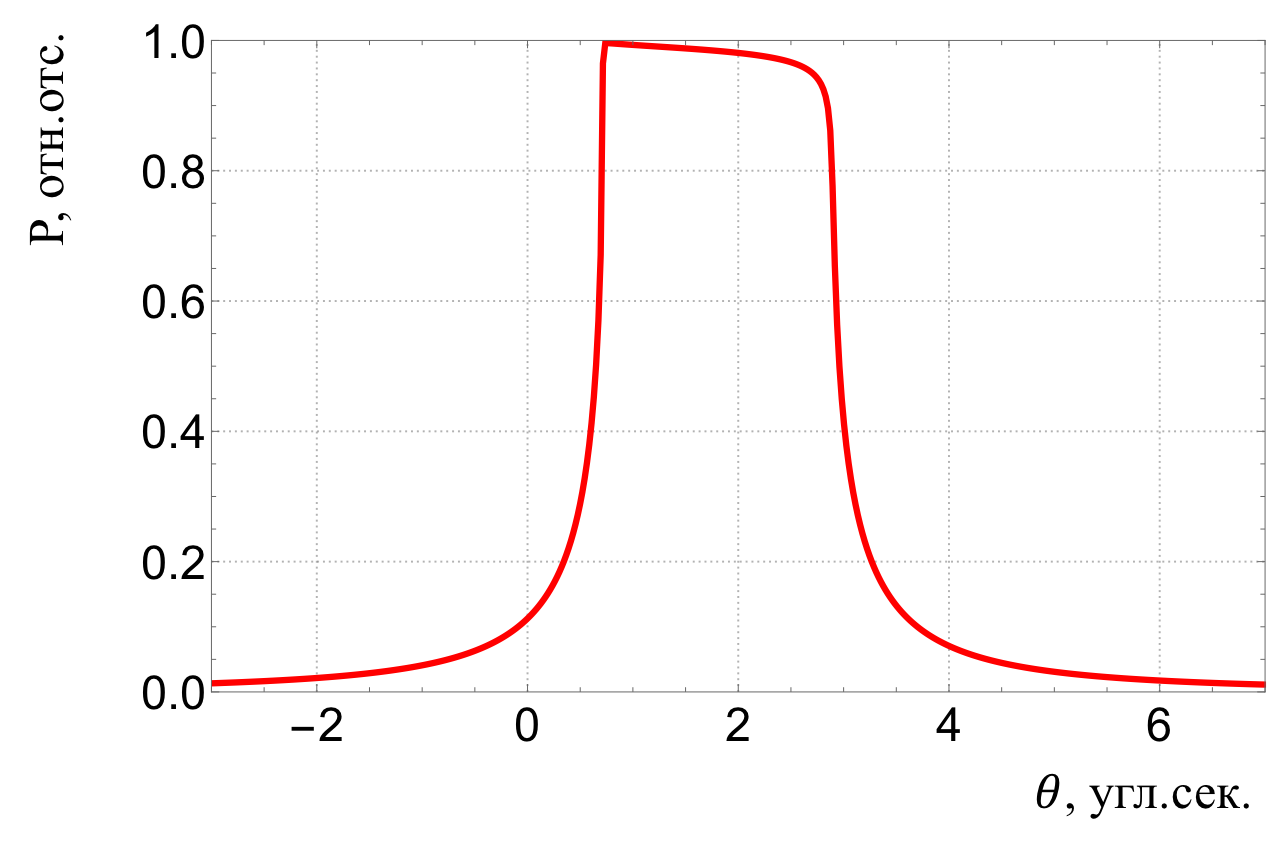
\includegraphics[width=0.45\textwidth]{images/darwin_si.png}\label{ris:darwin_si}}
  \hfill
  \subfloat[]{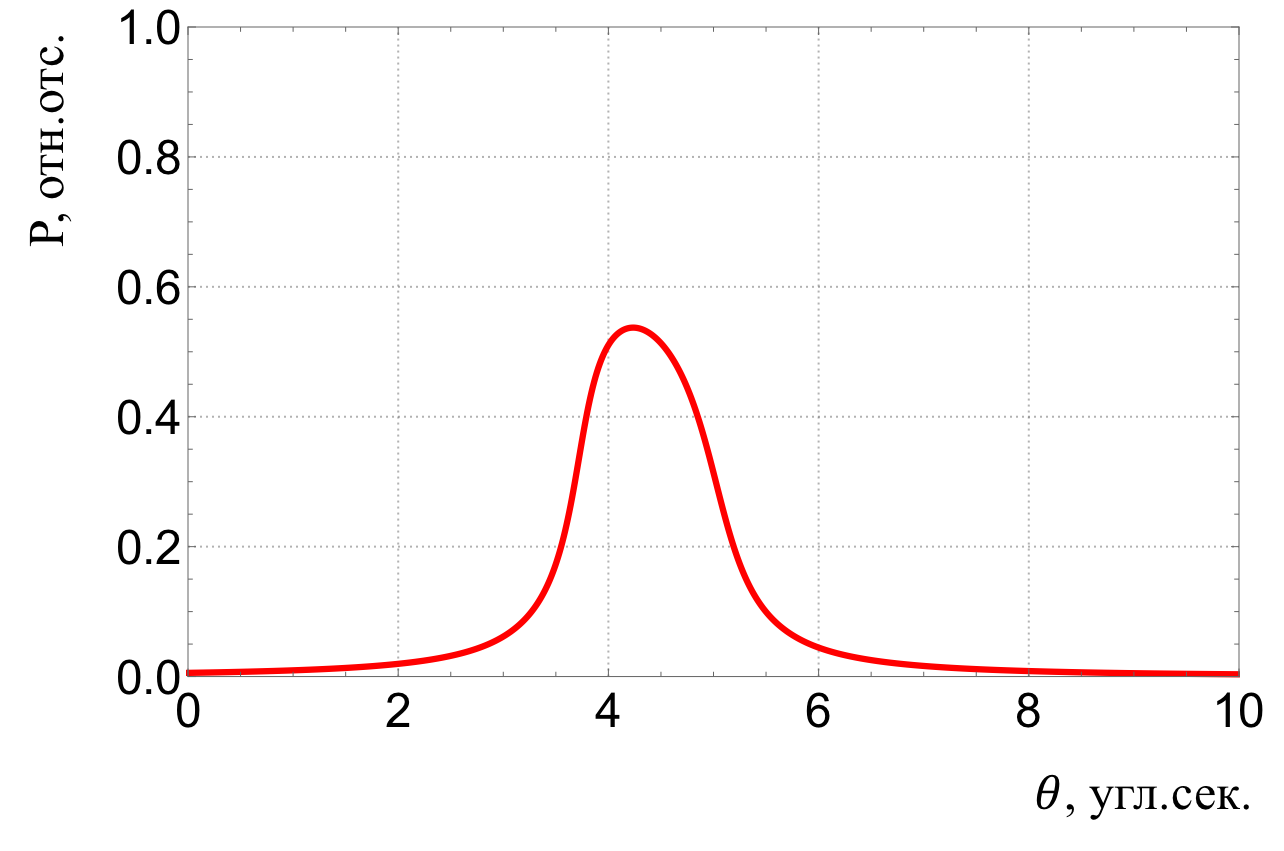
\includegraphics[width=0.45\textwidth]{images/darwin_lgt.png}\label{ris:darwin_lgt}}
  \caption{Собственная кривая отражения от кристалла Si(220) (a) и
  кристалла LGT(220) для $MoK_{\alpha 1}$ - излучения (b)}
  \label{ris:darwin_methody}
\end{figure}

В дальнейшем рассмотрении на спектрально-угловой карте будет присутствовать
полоса отражения от кристалла, которая представляет из себя набор собственных кривых с
разными углами Брэгга (рис. \ref{ris:darwin_lambda}).
Ширина полос на двумерной карте определяется полушириной (FWHM)
собственной кривой отражения.

\begin{figure}[H]
\centering
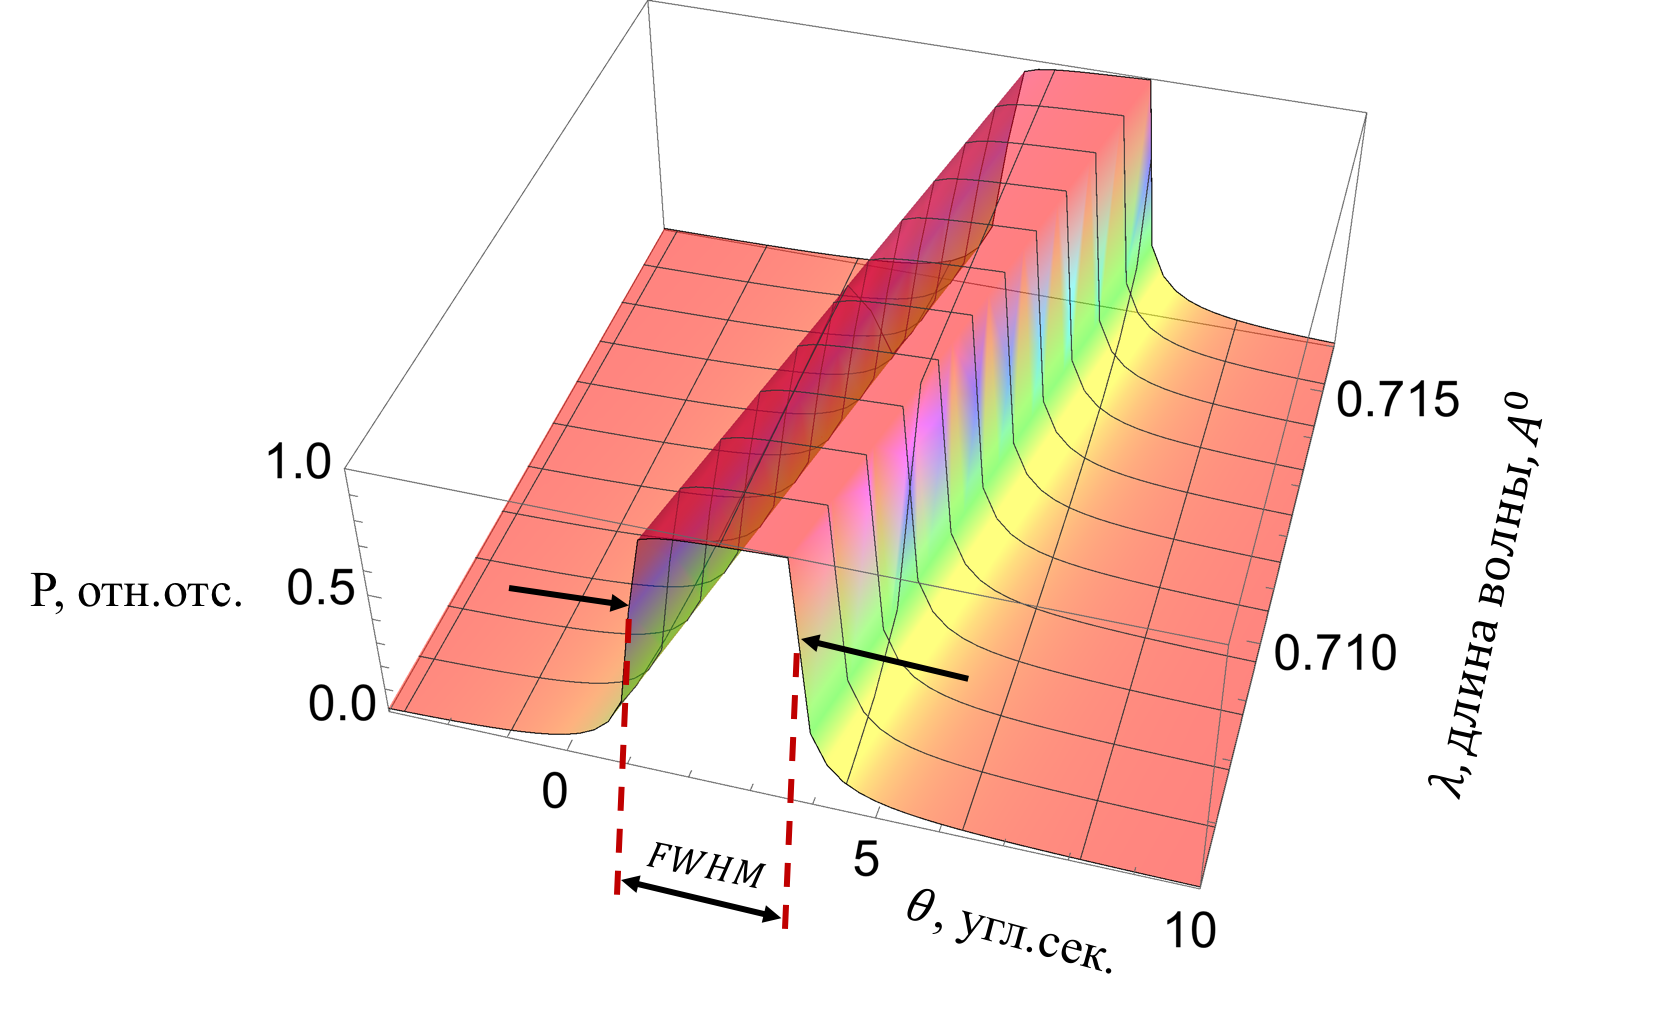
\includegraphics[width=0.7\textwidth]{images/darwin_lambda.png}
\caption{Полоса собственной КДО $MoK_{\alpha}$ - излучения
на спектрально-угловом распределении для кристалла
кремния  Si(220)  }
\label{ris:darwin_lambda}
\end{figure}

Весьма наглядной иллюстрацией влияния на собственную КДО асимметрии рефлекса являются
кривые отражения Si(440) рассчитанные при
трех разных углах падения и соответсвенно имеющие разный коэффициент асимметрии. Угол
Брэгга для такой плоскости отражения составляет $\theta_B = 21.68^o$, угол наклона поверхности
 по отношению к плоскостям (440) составляет $\varphi = 20^o 53^{'}$.

\begin{figure}[H]
\centering
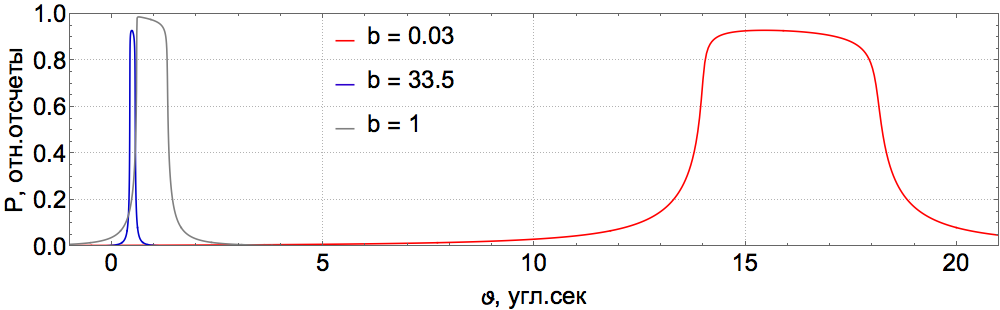
\includegraphics[width=0.99\textwidth]{images/rocking_curve_assym_3.png}
\caption{Кривые отражения от Si(440) $MoK_{\alpha 1}$ - излучения, полученные при разных углах падения(для разных b)}
\label{ris:rocking_curve_assym_3}
\end{figure}
Сдвиг центра кривой происходит из-за наличия преломления на величину 0.5 и 16.5 угловых секунд.
%
% Варьируя угол между поверхностью кристалла и отражающей плоскостью (например, с помощью шлифовки),
% можно существенно изменить ширину рентгеновского пучка (рис. ~\ref{ris:assym_width_beam}).
% \begin{figure}[H]
%  \centering
%  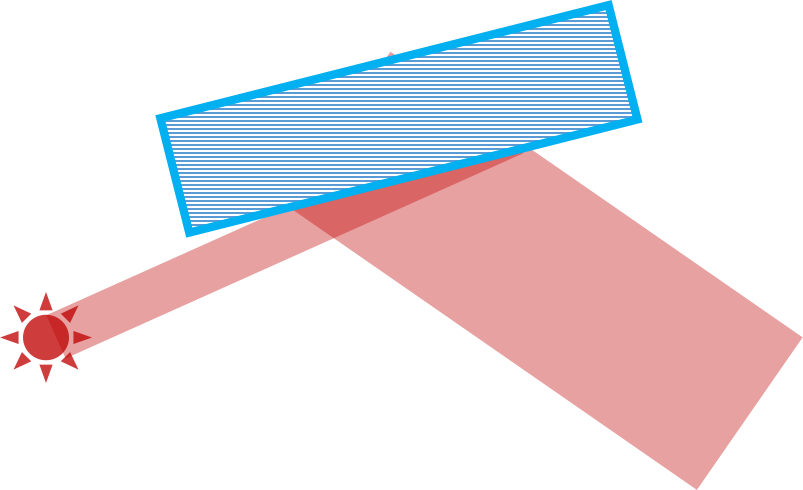
\includegraphics[width=0.4\textwidth]{images/assym_width_beam.png}
%  \caption{Кристалл с асимметричным отражением по Брэггу}
%  \label{ris:assym_width_beam}
% \end{figure}

    \subsubsection{Отражение от одного кристалла}
      \label{sec:single_crystal_section}

  Добавление в экспериментальную схему (рис. \ref{ris:for_slits}) кристалла - монохроматора
  наглядно демонтирует преимущество использования двумерных спектрально-угловых распределений.
Взаимодействие рентгеновского излучения с кристаллом определяется уже не только
угловой составляющей, но и спектральной.

  Спектрально-угловое распределение после отражения рентгеновского пучка от
  совершенного монокристалла задается выражением:
  \begin{equation} \label{eq:monochromator_spectra}
    P(\vartheta,\lambda) = g_{\lambda}(\lambda)g_{\vartheta}(\vartheta) P(\vartheta - \frac{\lambda - \lambda_1}{\lambda_1}\tg(\theta_B)),
   \end{equation}
где $P$ - соответствует (\ref{eq:KDO_self}), $\lambda_1$ - длина волны излучения, на которую
настраивается экспериментальная схема.

\begin{figure}[H]
  \centering
  \subfloat[]{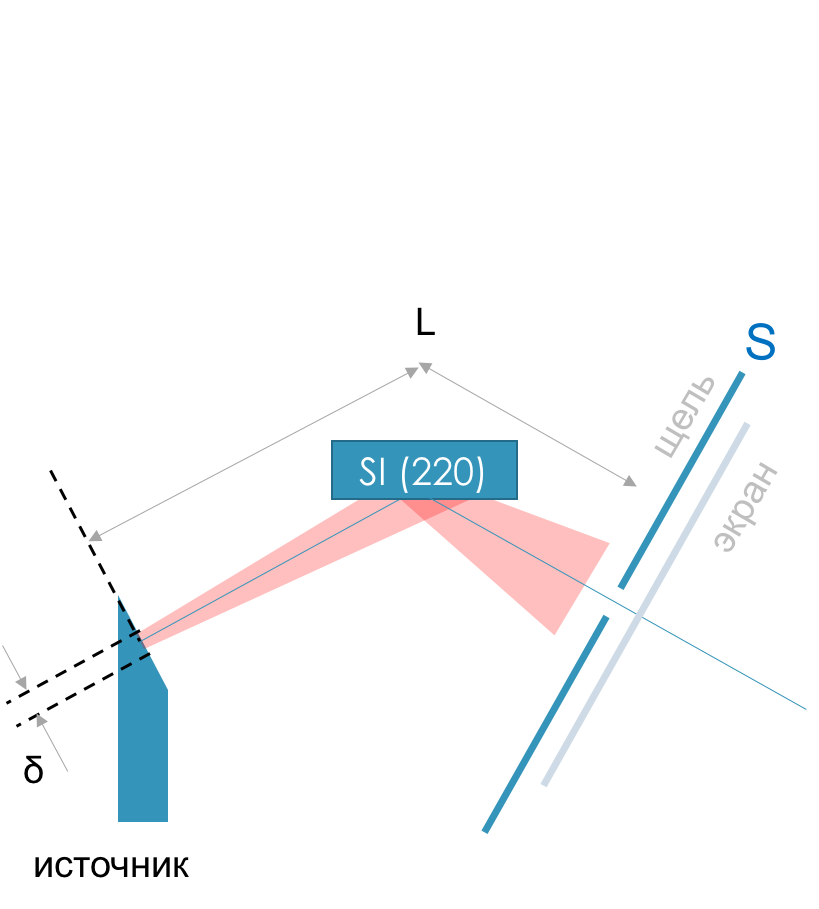
\includegraphics[width=0.45\textwidth]{images/single_crystal_schem.png}\label{ris:single_crystal_schem_lamtet_a}}
  \hfill
  \subfloat[]{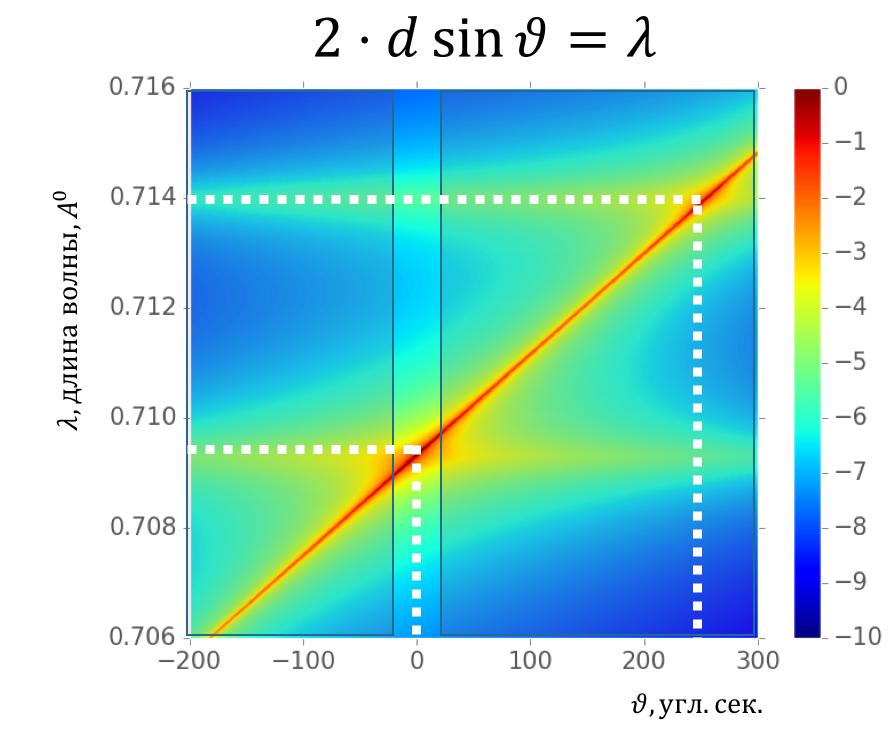
\includegraphics[width=0.45\textwidth]{images/single_crystal_schem_lamtet.png}}

  \caption{Схема однокристального эксперимента (a). Спектрально-угловое распределение
  рентгеновского излучения после отражения расходящегося характеристического излучения
  трубки с $Mo$ анодом от кристалла Si(220). Вертикальная полоса в окрестности
  $\vartheta = 0$ соответсвует угловому диапазону пропускания щелевых коллиматоров.(b)}
  \label{ris:single_crystal_schem_lamtet}
\end{figure}

Рис. \ref{ris:single_crystal_schem_lamtet} наглядно демонстрирует принцип работы
брэгговского монохроматора, когда после взаимодействия с кристаллом, разные
длины волн отражаются под разными углами в соответсвии с законом Вульфа-Брэгга.

Угловая зависимость отраженного монохроматором излучения с учетом прохождения
систем щелей задается следующим образом:

\begin{equation} \label{eq:p_single_crystal}
  P_{single}(\theta) = \sum_{\lambda = -\infty}^{\infty}g_{\lambda}(\lambda) \cdot \sum_{\vartheta = \vartheta_{s1}}^{\vartheta_{s2}}
  g_{\vartheta}(\vartheta) P_M(\vartheta - \frac{\lambda - \lambda_1}{\lambda_1}\tg(\theta_B)),
 \end{equation}
\noindent
где $\vartheta$ - угол падения излучения на кристалл, в случае не расходящегося пучка $\vartheta = 0$, в
случае, например, синхротронного источника $\vartheta \in (-6^o; 6^o) $; $g_{\lambda}(\lambda)$
- спектральная плотность распределения пучка (\ref{eq:source_spectral}); $g_{\vartheta}(\vartheta)$ - угловая плотность
распределения пучка (\ref{eq:source_angle}); $P_M$ - коэффициент отражения от кристалла-монохроматора,
слагаемое $\frac{\lambda - \lambda_1}{\lambda_1}\tg(\theta_B)$ - возникает из
условия Вульфа-Брэгга и описывает свойство разных длинн волн отражатся под разными углами.
 Суммирование проводится, во-первых, в пределах угловой апертуры детектора, которая задается размером
 щелевого коллиматора перед ним, с возможной отстройкой детектора от центрального положения
  $\vartheta_{s1} = \theta - \frac{S}{2L}$, $\vartheta_{s2} = \theta + \frac{S}{2L}$, где
   $S $ - линейный размер щелевого коллиматора, $L$ - расстояние от источника до щели.
 Во-вторых, суммирование осуществляется по всем $\lambda$, из-за свойства детектора не различать разные длины волн.
На рис. \ref{ris:zero_exp} приведен результат измерения углового распределения излучения рентгеновской трубки
после его отражения от неподвижного кристалла кремния Si(220) для разных размеров щелевого коллиматора
в сравнении с результатами моделирования для аналогичных параметров схемы.
Экспериментально измерять такую зависимость можно путем сканирования
детектором со щелью отраженного монохроматором пучка.

    \subsubsection{Методика моделирования двухкристальных кривых дифракционного отражения}
      

Измерение кривой дифракционного отражения в двухкристальной схеме представляет
собой измерение зависимости отраженного образцом рентгеновского излучения при
пошаговом повороте исследуемого кристалла относительно падающего на него
излучения в окрестности точного значения угла Брэгга.
Существует несколько схем измерения кривых отражения рентгеновского излучения.

\subsubsection*{$\omega$ - сканирование}
В данном типе сканирования кривая отражения измеряется путем поворота образца
относительно падающего пучка в плоскости дифракции. При таком сканировании
угол между падающим и дифрагированным пучками (угол рассеяния) остается постоянным
(рисунок ~\ref{ris:omega_scan}). Получаемая в результате кривая носит название кривой качания.


\begin{figure}[H]
  \centering
  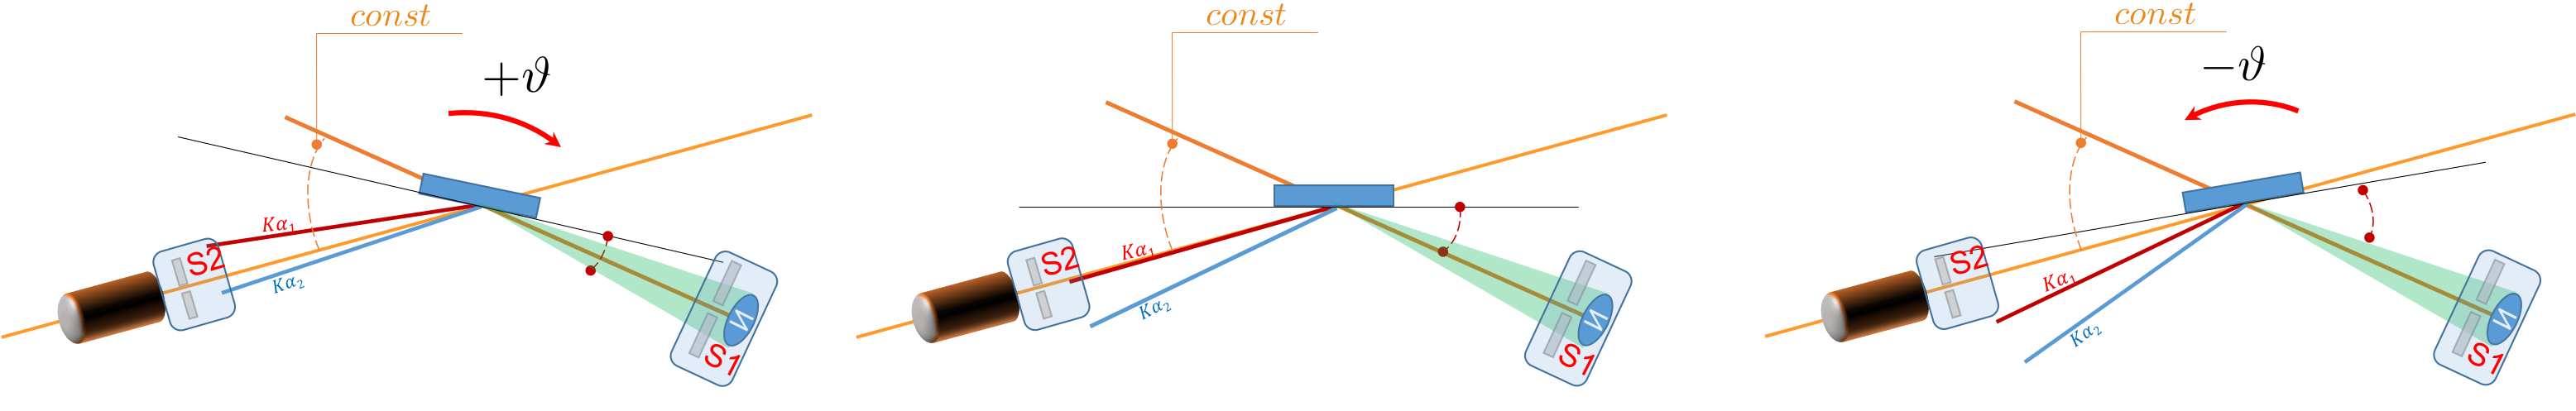
\includegraphics[width=1\textwidth]{images/omega_scan.png}
  \caption{Схема реализации $\omega $ - сканирования}
  \label{ris:omega_scan}
\end{figure}

\subsubsection*{$\vartheta - 2\vartheta$ - сканирование}
В отличие от предыдущего, данный метод сканирования соответствует изменению
 модуля вектора рассеяния при неизменном его угловом положении
 (рисунок ~\ref{ris:theta_2theta_scan}). Угловое положение падающего пучка и
 детектора изменяется синхронно и симметрично относительно используемой системы
 атомных плоскостей, а установленная перед детектором апертурная щель вырезает
  только зеркально отраженную часть пучка. Именно поэтому при построении карт
   пространственного распределения спектра полосы щелей на этих картах остаются
   неподвижными (т.к. несмотря на движение щели  $S_2$ в процессе
    $\vartheta - 2\vartheta$ -  сканирования ее отстройка от зеркального
    положения всегда равна 0).

 \begin{figure}[H]
   \centering
   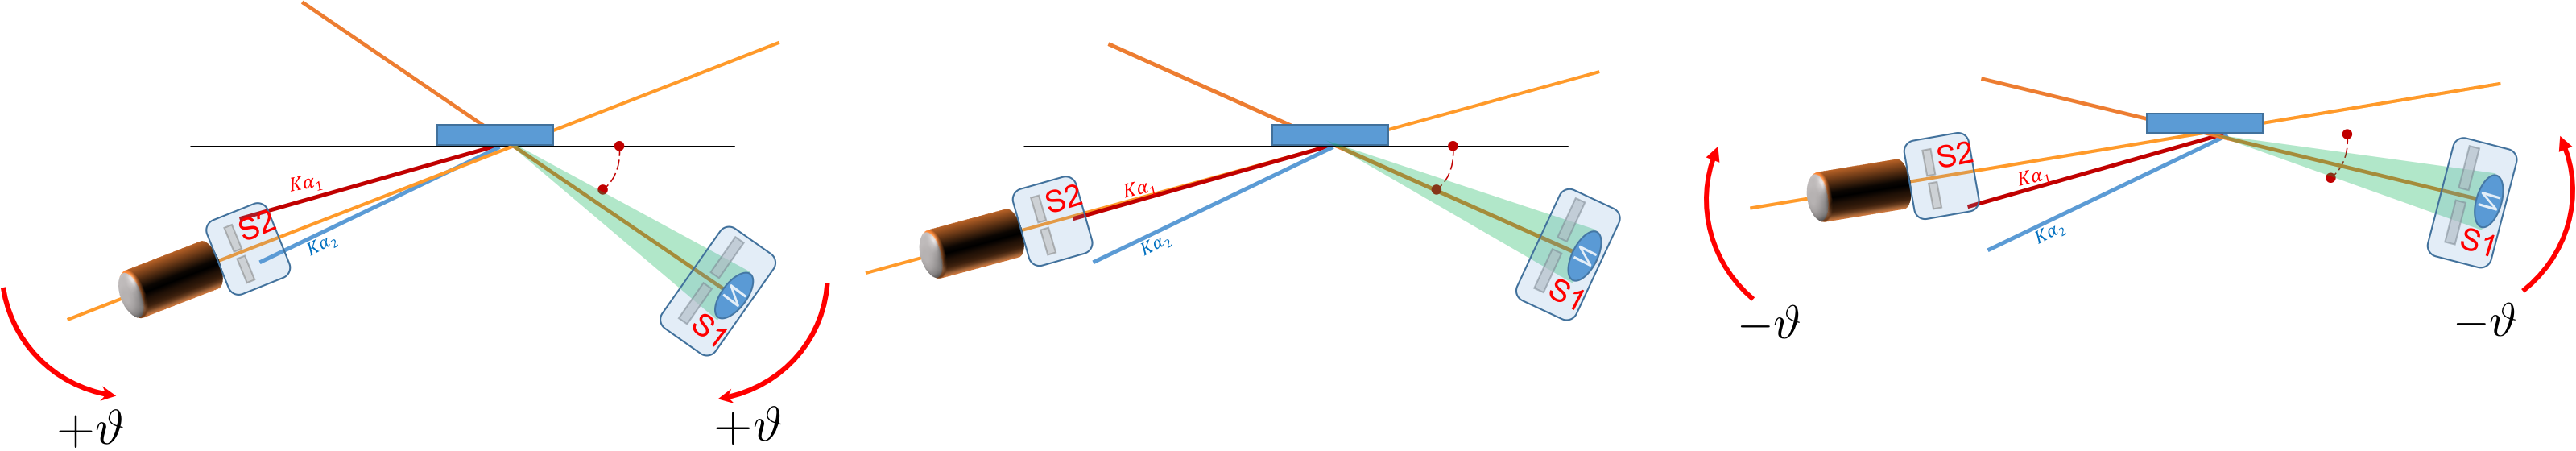
\includegraphics[width=1\textwidth]{images/theta_2theta_scan.png}
   \caption{Схема реализации $\vartheta - 2\vartheta$ - сканирования}
   \label{ris:theta_2theta_scan}
 \end{figure}
Кроме того, используемый подход позволяет наглядно продемонстрировать интересный эффект.
 Независимо от ширины входной и приемной щелей характеристическая линия спектра
 трубки $k_{\alpha 2}$ всегда вносит вклад в КДО, проявляясь в виде дополнительного
 пика на ее хвосте (рис. 2.21). Данный слабый пик возникает за счет того, что
 даже при очень малой входной щели $S_1$ линия $k_{\alpha 2}$ будет, отражаясь на «хвосте»
 кривой монохроматора, пролетать через входную щель и, при определённом угле
 поворота образца, интенсивно дифрагировать в максимуме его собственной кривой
 отражения и давать весомый ($~10^{-6}$) вклад в общую интенсивность КДО.

    \subsubsubsection*{Выражение для расчета двухкристальных КДО}
      
Для того, чтобы разобраться в том, как формируются экспериментальные
двухкристальные КДО, нам необходимо построить спектрально-угловое распределение
в соответствии со схемой эксперимента (рисунок \ref{ris:double_crystal_schem_lamtet_a}).

\begin{eqnarray} \label{eq:doudle_spectra_angle_map}
  P(\theta,\vartheta,\lambda) = g_{\lambda}(\lambda)g_{\vartheta}(\vartheta) P_M \left(\vartheta - \frac{\lambda - \lambda_1}{\lambda_1}\tan(\theta_B) \right) \cdot \nonumber \\
   P_S \left(\theta + \vartheta - \frac{\lambda - \lambda_1}{\lambda_1}\tan(\theta_B)\right)
 \end{eqnarray}

Выражение (\ref{eq:doudle_spectra_angle_map}) определяет спектрально угловое распределение после прохождения двух кристаллов с
коэффициентами отражения  $P_M$ (монохроматор) и $P_S$ (образец), причем последний принимает во внимание положение угла отстройки $\theta$ относительно
точного Брегга (рисунок \ref{ris:double_crystal_schem_lamtet_b}).

\begin{figure}[H]
  \centering
  \subfloat[Схема двухкристального эксперимента]{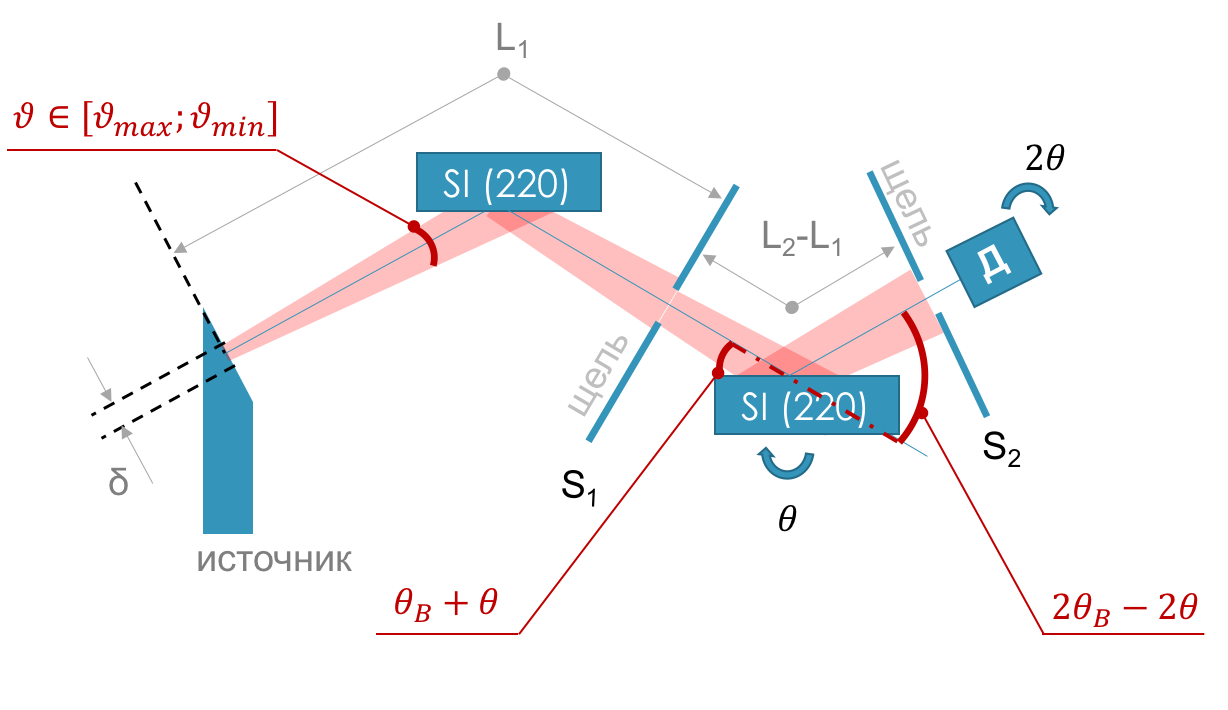
\includegraphics[width=0.5\textwidth]{images/double_crystal_schem.png}\label{ris:double_crystal_schem_lamtet_a}}
  \hfill
  \subfloat[Спектрально угловое распределение. Положение щелевых устройств обозначено синей и белой линиями вблизи $\vartheta = 0$ угл.сек. Кристалл-образец
  выведен из точного Брегговского положения на 300 угл. сек.
   ]{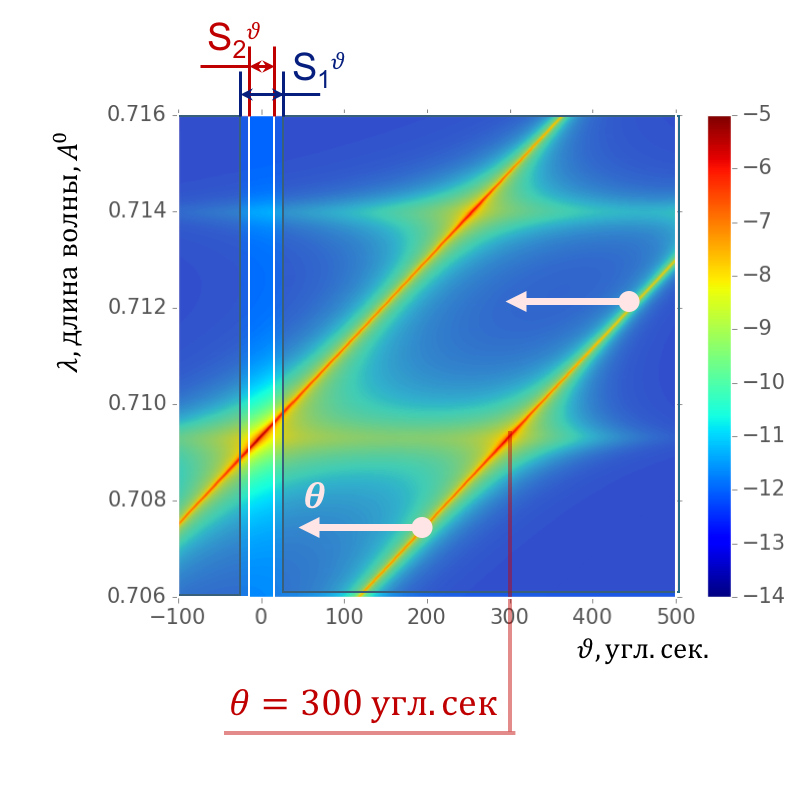
\includegraphics[width=0.45\textwidth]{images/double_crystal_schem_lamtet.png} \label{ris:double_crystal_schem_lamtet_b}}

  \caption{Схема и спектрально-угловое распределение после отражения расходящегося, полихромотического пучка. Несмотря на то, что в
  экспериментальной схеме детектор со щелью не стоят на месте, на карте обе щели $S_1$ и $S_2$ - неподвижны. }
  \label{ris:double_crystal_schem_lamtet}
\end{figure}

Выражение (\ref{eq:doudle_spectra_angle_map}) не учитывает особенности особенности влияния щелевых коллиматоров, о которым мы говорили в
(раздел \ref{sec:slits_section}), а так же тот факт, что детектор не разделят энергетическую составляющую пучка.


\begin{eqnarray} \label{eq:doudle_spectra_angle_map_on_detector}
  P_{double}(\theta) = \sum_{\lambda = -\infty}^{\infty}g_{\lambda}(\lambda)\cdot
  \sum_{\vartheta = \vartheta_{s1}}^{\vartheta_{s2}} g_{\vartheta}(\vartheta) g_{S}(\vartheta) \cdot \nonumber \\
   P_M \left(\vartheta - \frac{\lambda - \lambda_1}{\lambda_1}\tan(\theta_B) \right) \cdot \nonumber \\
   P_S \left(\theta + \vartheta - \frac{\lambda - \lambda_1}{\lambda_1}\tan(\theta_B)\right)
 \end{eqnarray}
 где пределы суммирования определяются как $\vartheta_{s2} = - \vartheta_{s1} = \frac{\delta+S_1}{2L_1}$.

 \begin{figure}[H]
   \centering
   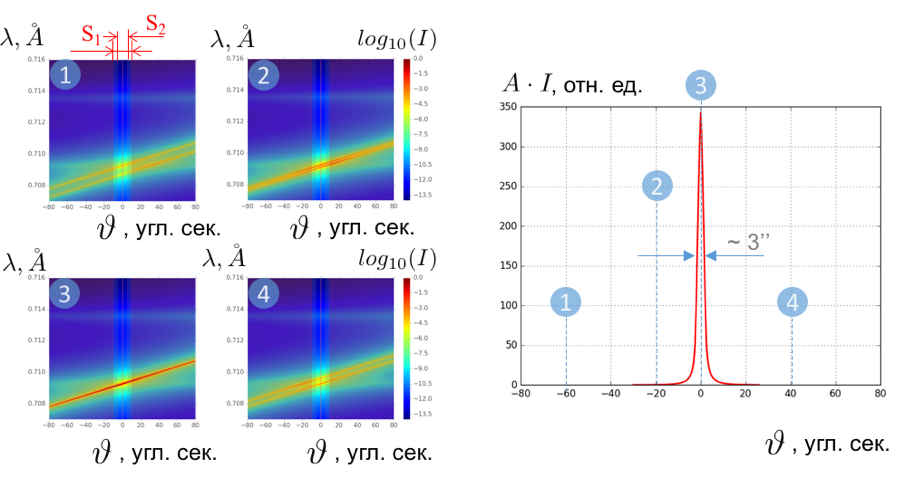
\includegraphics[width=1\textwidth]{images/double_crystal_form_kdo.png}
   \caption{Формирование двухкристальной кривой дифракционного отражения ($\theta - 2\theta$ - cканирование),
   $\theta_B^M = \theta_B^S = 10.6^o$  }
   \label{ris:double_crystal_form_kdo}
 \end{figure}

В том случае, если схема дисперсионная т.е. углол Брегга кристалла - образца отличен от угла Брега кристалла-монохроматора,
наблюдается уширения двухкристальных кривых (рисунок \ref{ris:double_crystal_form_kdo_dissp}).
 \begin{figure}[H]
   \centering
   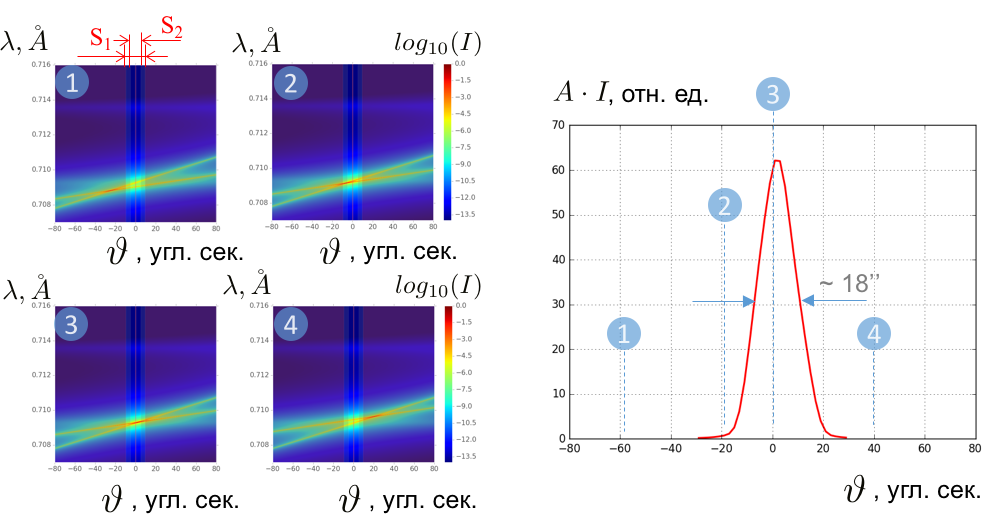
\includegraphics[width=1\textwidth]{images/double_crystal_form_kdo_dissp.png}
   \caption{Формирование двухкристальной кривой дифракционного отражения ($\theta - 2\theta$ - cканирование) в случае
   наличия дисперсии, $\theta_B^M = 10.6^o$, $\theta_B^S = 21.6^o$ }
   \label{ris:double_crystal_form_kdo_dissp}
 \end{figure}

    \subsubsection{Методика моделирования трехкристальных кривых дифракционного отражения}
      \subsubsubsection{Карта рассеяния в прямом пространстве}
        На кристалл монохроматор (M) падает расходящийся набор рентгеновских лучей, каждый из которых характеризуется отстройкой
$\vartheta$ от точного брэгговского направления (рис. \ref{ris:triple_crystal_schem}). Отраженный луч с интенсивностью
$I_0 P_M(\vartheta)$ далее падает на образец и дальше $I_0 P_M(\vartheta)P_S(\vartheta)$  на анализатор $I_0 P_M(\vartheta)P_S(\vartheta)P_A(\vartheta)$,
сохраняя величину отстройки.

Необходимо также ввести угловые отстройки от точного брэгговского положения
для образца (S) $\theta$ и анализатора (A) $\varepsilon$  (углы отсчитываются в сторону увеличения угла падающего луча).
В результате поворота образца на угол  $\theta$ излучение отраженное от монохроматора, падает на образец
под углом $\theta_B+\theta+\vartheta$. Если кристалл повернуть на угол $\theta$, отраженный повернется на удвоенный угол
$2\theta$, в итоге излучение падает на анализатор (А) под углом $\theta_B+2\theta-\varepsilon+\vartheta$ \cite{trd_Bushuev_1997}.
\begin{figure}[H]
  \centering
  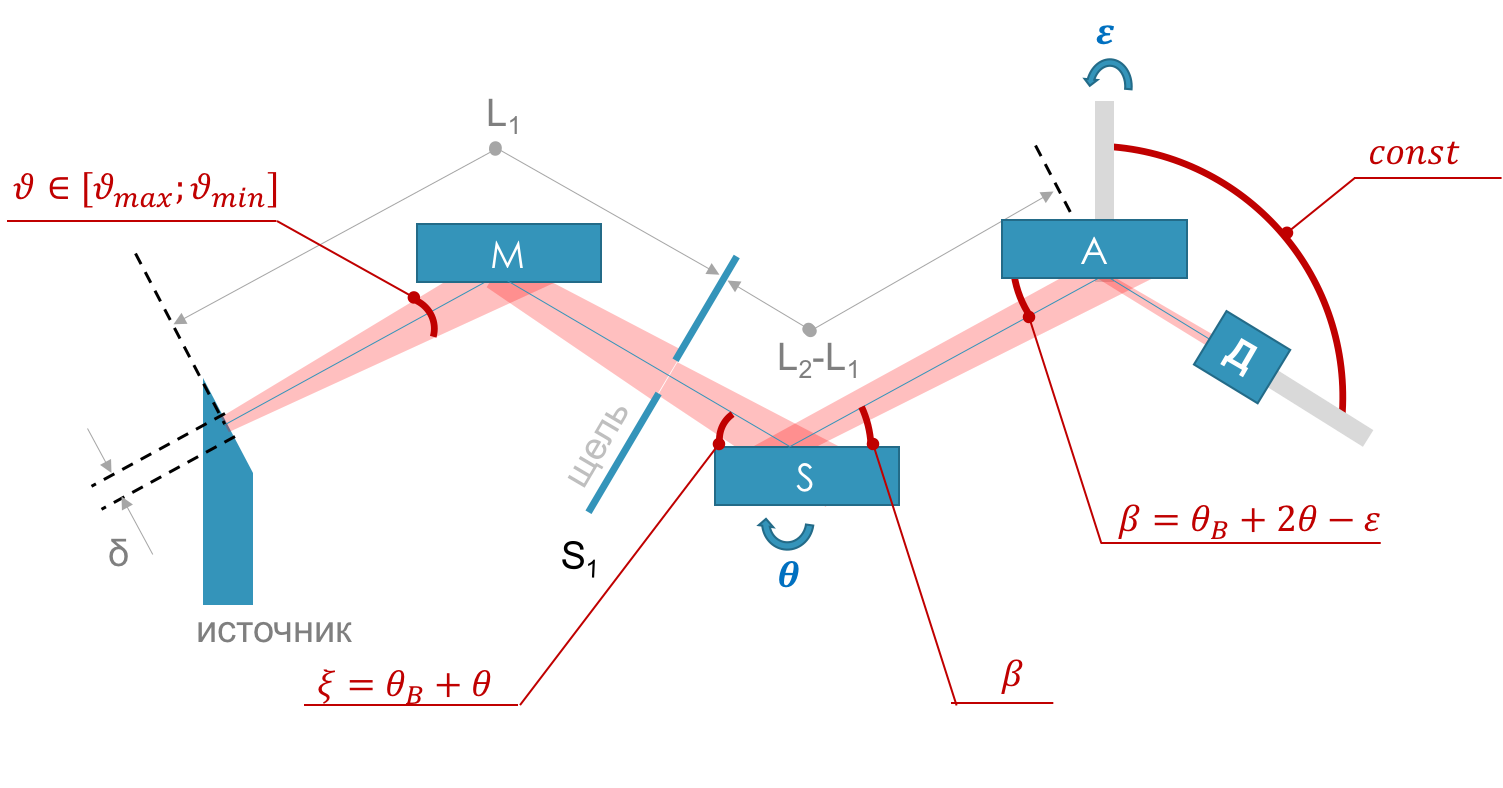
\includegraphics[width=0.8\textwidth]{images/triple_crystal_schem.png}
  \caption{Схема трехкристального эксперимента, $\theta$ - отстройка образца от точного угла Брэгга,
  $\varepsilon$ - угол отстройки анализатора относительно положения оптической оси}
  \label{ris:triple_crystal_schem}
\end{figure}

Учитывая что рентгеновская трубка имеет полихроматический спектр, лучи падающие под разными углами могут отражаться
с одинаковым коэффициентом отражения за счет разной энергии $\frac{\lambda - \lambda_1}{\lambda_1}\tan(\theta_B)$,
спектрально угловое распределение, исходя из вышесказанного, задается выражением:

\begin{eqnarray} \label{eq:triplr_spectra_angle_map}
  P_{triple}(\vartheta,\lambda,\theta,\varepsilon) =I_0\cdot
    P_M \left(\vartheta - \frac{\lambda - \lambda_1}{\lambda_1}\tan(\theta_B) \right) \cdot \nonumber \\
   P_S \left(\theta + \vartheta - \frac{\lambda - \lambda_1}{\lambda_1}\tan(\theta_B)\right)  \cdot  \nonumber \\
   P_A \left(2\theta - \varepsilon + \vartheta - \frac{\lambda - \lambda_1}{\lambda_1}\tan(\theta_B)\right) \Bigg]
 \end{eqnarray}

  \begin{figure}[H]
    \centering
    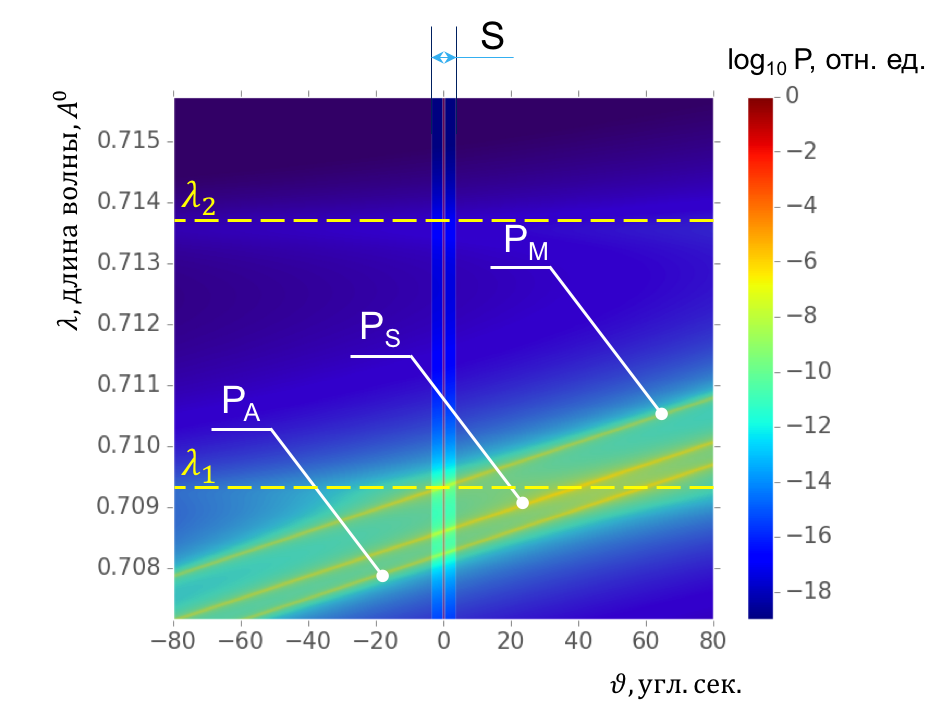
\includegraphics[width=0.6\textwidth]{images/triple_map.png}
    \caption{Спектрально-угловое распределение для случая наличия трех кристаллов в схеме для
    лабораторного источника с молибденовым анодом.
    Прямая образца отстроена на $\theta = - 50''$, анализатора на $\varepsilon = 20''$ относительно
    зеркально отраженного луча после кристалла-образца. Так же на схеме изображено щелевое устройство размером около 7 $''$}
    \label{ris:triple_map}
  \end{figure}

Анализ движения прямых отражения на спектрально-угловом распределении (рис. \ref{ris:triple_map}) от угла отстройки образца $\theta$ и
анализатора $\varepsilon$ показывает, что суммарная интенсивность зафиксированная детектором внутри щелевого устройства
$S$ имеет вид пикообразной кривой состоящей из трех максимумов (рис. \ref{ris:triple_map_piks}).

\begin{figure}[H]
  \centering
  \subfloat[]{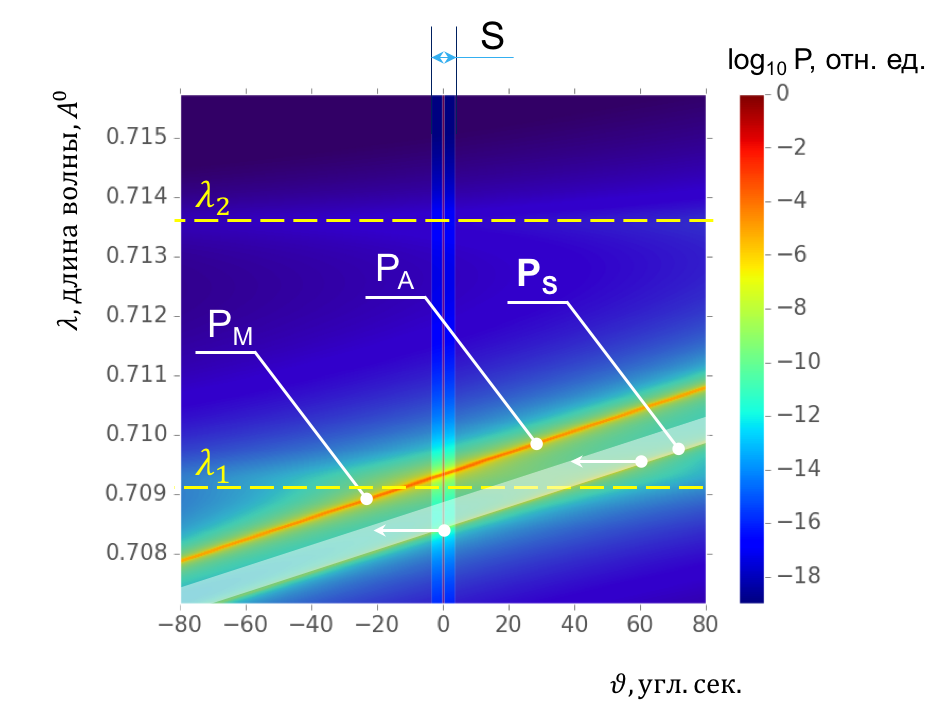
\includegraphics[width=0.32\textwidth]{images/triple_map_g.png}\label{ris:triple_map_piks_g}}
  \hfill
  \subfloat[]{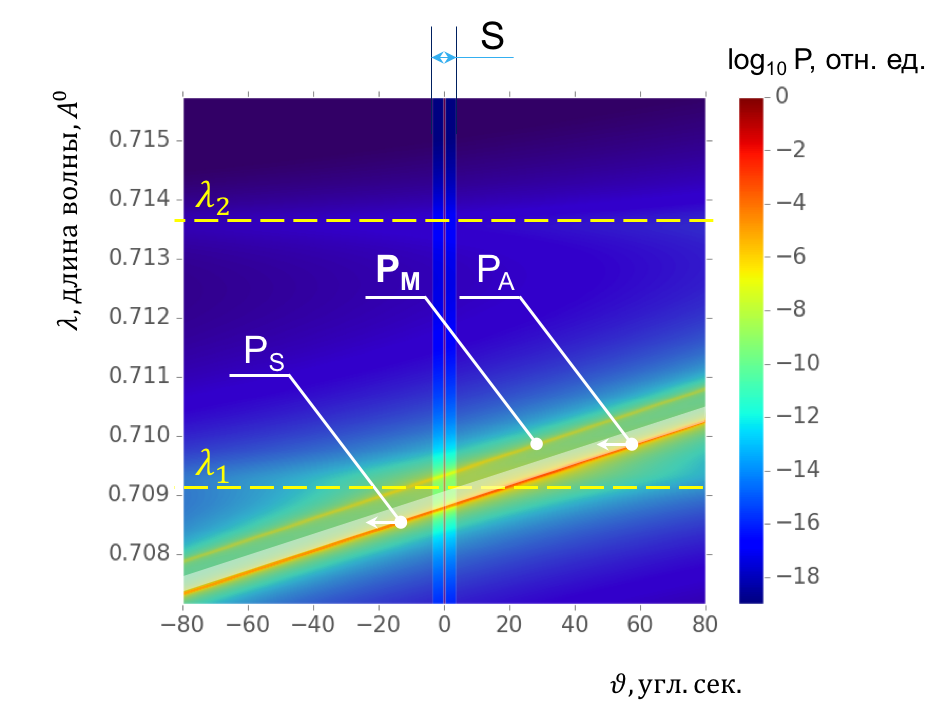
\includegraphics[width=0.32\textwidth]{images/triple_map_m.png} \label{ris:triple_map_piks_m}}
  \hfill
  \subfloat[]{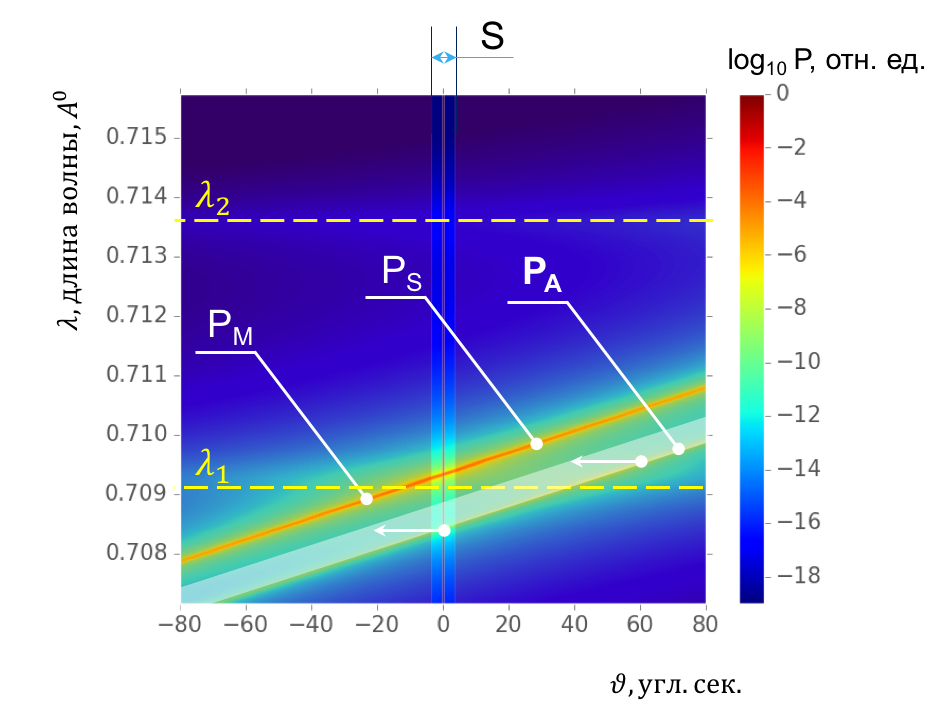
\includegraphics[width=0.32\textwidth]{images/triple_map_a.png} \label{ris:triple_map_piks_a}}
  \caption{Формирование карты рассеяния в прямом пространстве, вдоль направления (a) главного пика,
  (b) псевдо пика монохроматора, (c) псевдо пика анализатора}
  \label{ris:triple_map_piks}
\end{figure}

Максимальная интенсивность в случае сканирования по всем углам отстройки кристалла - образа и
 кристалла - монохроматора
возникает в том случае, когда две из трех прямых, соответствующих коэффициентам отражения от кристаллов,
находятся на одном угловом положении (рис. \ref{ris:triple_map_piks}), а третья осуществляет движение.

\subsubsection*{Главный пик}
Главный пик (ГП) формируется в случае отстройки кристалла-образца от точного угла Брэгга,
максимум при $|\theta|>>0''$ имеет место при повороте анализатора на $\varepsilon = 2\theta$,
тогда выражение (\ref{eq:triplr_spectra_angle_map}) примет частный вид

\begin{eqnarray} \label{eq:triplr_spectra_angle_map_GP}
  P_{\text{ГП}}(\vartheta,\lambda,\theta,\varepsilon) =I_0\cdot
    P_M \left(\vartheta - \frac{\lambda - \lambda_1}{\lambda_1}\tan(\theta_B) \right) \cdot \nonumber \\
   P_S \left(\theta + \vartheta - \frac{\lambda - \lambda_1}{\lambda_1}\tan(\theta_B)\right)  \cdot  \nonumber \\
   P_A \left(0+\vartheta - \frac{\lambda - \lambda_1}{\lambda_1}\tan(\theta_B)\right) \Bigg]
 \end{eqnarray}
как видно на рис. \ref{ris:triple_map_piks_g}, прямая анализатора и образца перекрывают друг друга и пик формируется
движением прямой образца. Такой режим сканирования в экспериментальной практике называется $\theta-2\theta$ сканированием,
угол поворота кристалла образца соответствует удвоенному повороту анализатора. В этом случае мы движемся
вдоль пика чисто когерентного рассеяния, т.е. направляя на образец луч с конкретными значением отстройки $\vartheta$ и энергией соответствующей
 $\lambda$, а дальше анализируем отраженный луч, с той же энергией и угловой составляющей. Для примера, это
 будет показано дальше, образец с измененным межплоскостным расстоянием будет смещать максимум отражения именно вдоль направления
 главного (когерентного) пика.

\subsubsection*{Пседво пик монохроматора}
Псевдо пик монохроматора (ППМ) (рис. \ref{ris:triple_map_piks_m}) формируется когда прямые образца и анализатора
двигаются вместе, перекрываясь между собой. Угол отстройки образца и анализатора совпадает $\theta = \varepsilon$.

\begin{eqnarray} \label{eq:triplr_spectra_angle_map_PPM}
  P_{\text{ППМ}}(\vartheta,\lambda,\theta,\varepsilon = \theta) =I_0\cdot
    P_M \left(\vartheta - \frac{\lambda - \lambda_1}{\lambda_1}\tan(\theta_B) \right) \cdot \nonumber \\
   P_S \left(\theta + \vartheta - \frac{\lambda - \lambda_1}{\lambda_1}\tan(\theta_B)\right)  \cdot  \nonumber \\
   P_A \left(\theta  + \vartheta - \frac{\lambda - \lambda_1}{\lambda_1}\tan(\theta_B)\right) \Bigg]
 \end{eqnarray}

 \subsubsection*{Пседво пик анализатора}
 Псевдо пик анализатора (ППА) формируется когда монохроматор и образец
 находятся в точном брэгговском положении, перекрываясь между собой. Движение вдоль ППА осуществляется
 движением анализатора  на карте спектрально углового распределения (рис. \ref{ris:triple_map_piks_a}).
   Угол отстройки образца и анализатора совпадает $\theta = 0$.

 \begin{eqnarray} \label{eq:triplr_spectra_angle_map_PPM}
   P_{\text{ППА}}(\vartheta,\lambda,\theta=0,\varepsilon) =I_0\cdot
     P_M \left(\vartheta - \frac{\lambda - \lambda_1}{\lambda_1}\tan(\theta_B) \right) \cdot \nonumber \\
    P_S \left(0 + \vartheta - \frac{\lambda - \lambda_1}{\lambda_1}\tan(\theta_B)\right)  \cdot  \nonumber \\
    P_A \left(0-\varepsilon  + \vartheta - \frac{\lambda - \lambda_1}{\lambda_1}\tan(\theta_B)\right) \Bigg]
  \end{eqnarray}


\subsubsection*{Интенсивность на детекторе}

Необходимо учитывать что детектирующее устройство суммирует всю интенсивность в пределах своей аппертуры и по всем длина волн,
таким образом выражения для распределения интенсивности в методе трехкристальной рентгеновской дифракции имеет следующий
общий вид:

\begin{eqnarray} \label{eq:doudle_spectra_angle}
  P_{triple}(\theta,\varepsilon) = \sum_{\lambda = -\infty}^{\infty}g_{\lambda}(\lambda)\cdot
  \sum_{\vartheta = \vartheta_{s1}}^{\vartheta_{s2}} \Bigg[ g_{\vartheta}(\vartheta) g_{S}(\vartheta) \cdot \nonumber \\
    P_M \left(\vartheta - \frac{\lambda - \lambda_1}{\lambda_1}\tan(\theta_B) \right) \cdot \nonumber \\
   P_S \left(\theta + \vartheta - \frac{\lambda - \lambda_1}{\lambda_1}\tan(\theta_B)\right)  \cdot  \nonumber \\
   P_A \left(2\theta - \varepsilon + \vartheta - \frac{\lambda - \lambda_1}{\lambda_1}\tan(\theta_B)\right) \Bigg]
 \end{eqnarray}
 \noindent
где пределы суммирования определяются щелевым коллиматором $\vartheta_{s2} = - \vartheta_{s1} = \frac{\delta+S_1}{2L_1}$.
 \begin{figure}[H]
   \centering
   \includegraphics[width=0.6\textwidth]{images/triple_map_direct_space.png}
   \caption{Трехкристальная карта распределения в пространстве углов отстройки $\theta$ - образца и $\varepsilon$
   -  анализатора}
   \label{ris:triple_map_direct_space}
 \end{figure}

Анализ показывает, что ГП находится под углом $60^o$, т.к. сканирование осуществляется вдоль $\varepsilon = 2 \theta$,
а $ \arctan \left(\frac{\varepsilon}{\theta} \right) = 63.4^o$. ППМ образует угол $45^o$, т.к. $\varepsilon = \theta$.

      \subsubsubsection{Карта рассеяния в обратном пространстве}
        Удобным для интерпретации является построение трехкристальных карт в обратном пространстве.  Таким
образом мы становимся не зависимыми от наличия разных типов дифрактометров, в одних из которых
формирование главного пика осуществляется поворотом образца и поворотом на двойной угол анализатора (ТРС),
в других же дифрактометрах (Rigaku) образец в процессе такого сканирования остается в статичном положении,
а поворачивается источник и детектор на одинаковые углы. Угловые положения падающего пучка и анализатора
определяет вектор рассеяния $\vec{q}$, такой вектор можно разложить на составляющие: $q_z$ - вертикальную составляющую,
направленную перпендикулярно от поверхности отражающей плоскости и $q_x$ - горизонтальную составляющую,
лежащую в отражающей плоскости (рисунок \ref{ris:q_vector_reciprocal_space}).

\begin{figure}[H]
  \centering
  \subfloat[Точное бреговское положение]{\includegraphics[width=0.3\textwidth]{images/q_vector/0.png}}
  \hfill
  \subfloat[Около брегговское положение - деформация]{\includegraphics[width=0.3\textwidth]{images/q_vector/_1.png}}
  \hfill
  \subfloat[Около брегговское положение - разориентация]{\includegraphics[width=0.3\textwidth]{images/q_vector/1.png}}
  \caption{Отклонение вектора обратной решетки от точного положения}
  \label{ris:q_vector_reciprocal_space}
\end{figure}

Для симметричного отражения эти составляющие связаны с отклонением образца $\theta$ и
анализатора $\varepsilon$ от нулевых положений в номинальном угле Брегга следующими
уравнениями \cite{Tanner_1998}:

\begin{equation}
  q_x = \frac{\varepsilon}{|\vec{k}_0|} \cos \theta_B
  \label{eq:qx_eqn}
\end{equation}

\begin{equation}
  q_z = \frac{2\theta - \varepsilon}{|\vec{k}_0|} \sin \theta_B
  \label{eq:qz_eqn}
\end{equation}

Таким образом, сканирование образцом влияет только на $q_y$ - слева направо в обратном пространстве.
Сканирование анализатора влияет на оба вектора, изменение только одного $q_z$ достигается за
счет $\theta-2\theta$ сканирования.

\begin{figure}[H]
  \centering
  \includegraphics[width=0.6\textwidth]{images/triple_map_reciprocal_space.png}
  \caption{Карта рассеяния в обратном пространстве}
  \label{ris:triple_map_reciprocal_space}
\end{figure}

Угол между ГП и ПП определяется исходя из соотношений (\ref{eq:qx_eqn}, \ref{eq:qz_eqn}) и равен углу Брегга образца:

\begin{equation}
  \frac{q_y}{q_z} = \frac{2\theta - \varepsilon}{\varepsilon} \cdot \tan (\theta_B) = \pm \tan (\theta_B)
  \label{eq:qz_eqn}
\end{equation}

    \subsubsection{Методика расчета пьзоэлектрических констант по данным дифракции}
      Согласно сказанному в (\ref{sec:piezo_theor}), в определенных кристаллографических направлениях в
условия воздействия внешнего электрического поля, будет возникать деформация
сжатия или растяжения. Этим деформациям соответсвует изменение межплоскостных
 расстояний, которое может быть измерено с помощью дифракции рентгеновского
 излучения по изменению угла Брегговского пика \cite{marchenkov2014}.

Исходя из закона Вульфа - Брегга, если межплоскостное расстояние получило приращение
$\Delta d$, тогда изменение угла отражения $\Delta \theta$ составит:

$$ \Delta d = \frac{\lambda}{2}\left( \frac{1}{\sin(\theta_B + \Delta \theta) } - \frac{1}{\sin \theta_B } \right) $$

\begin{equation}
   \Delta \theta =-  \frac{\tan \theta_B}{\frac{d}{\Delta d}+1}  = -  \frac{\Delta d }{d}  \tan \theta_B
\end{equation}
где $\Delta d/d = r$ - изменение межплоскостного расстояния. Таким образом, учитывая связь с
(\ref{eq:piezomodule}), для напряженности электрического поля $E = \frac{V}{L}$ для
 кристалла толщиной $L$ и разностью потенциалов на его гранях $V$ пьезоэлектрический модуль
 рассчитывается исходя из следующего выражения

 \begin{equation}
    d_{ij} = -\frac{\Delta \theta \cdot L_i}{V \tan \theta_B^i}
 \end{equation}

      \subsubsection{Методика экспериментального определения
      пльзоэлектрических констант по данным рентгеновской дифракции}
        \subsubsubsection{Статический метод}
            Метод двухкристальной дифрактометрии широко распространен для исследования пьезоэлектрических свойств \cite{piezo51} - \cite{piezo54}.
Для того, чтобы зафиксировать смещение пика двухкристальной КДО, необходимо проснять кривую дифракционного отражения
до и после приложенного напряжения (рисунок \ref{ris:piezo_classic}).
\begin{figure}[H]
  \centering
  \subfloat[В отсутствии поля]{\includegraphics[width=0.33\textwidth]{images/piezo_classic_1.png}\label{ris:piezo_classic_1}}
  \hfill
  \subfloat[Под действие элекрического поля]{\includegraphics[width=0.33\textwidth]{images/piezo_classic_2.png}\label{ris:piezo_classic_2}}
  \hfill
  \subfloat[Изменение положения максимума КДО]{\includegraphics[width=0.2\textwidth]{images/piezo_classic_3.png}\label{ris:piezo_classic_3}}

  \caption{Схематичное представление методики измерения сдвига брегговского максимума}
  \label{ris:piezo_classic}
\end{figure}
  Такой метод не позволяет отследить динамику какую - либо динамику в момент приложения электрического поля,
  т.к. время за которое получается КДО составляет десятки секунд на лабораорном источнике.

        \subsubsubsection{Времяразрешающий метод}
            \label{sec:slope_diff_piezo}
Другой метод, предложенный авторами \cite{piezo50}, заключается в измерении интенсивности
дифрагированного образцом излучения при фиксированной отсройке от точного
брэговского угла кристалла образца в двухкристальной геометрии.
% Необходимо  встать в произвольную точку на кривой дифракционного отражения,
% другими словами выведем интенсивность детектора из максимума отражения в точку на склоне
%  кривой (Рис.~\ref{ris:kdopiez}).

\begin{figure}[H]
\centering
\includegraphics[width=1\linewidth]{images/kdopiez2.png}
\caption{Отстройка кристалла из точного брэгговского положения в положение,
соответствующее склону КДО (а) и соответствующее изменение интенсивности сигнала на детекторе (b)}
\label{ris:kdopiez}
\end{figure}
\noindent
Другими словами, необходимо выставить образец в угловое положение, соответсвующее склону КДО.
В таком случае, при смещении КДО в результате пьзоэффекта будет наблюдаться резкое изменение
интенсивности при неподвижном образце, т.е при таком подходе даже не требуется проводить
измерение КДО, зная точно ее форму и скачок интенсивности вызванный внешним воздействием.
Несмотря на то, что данный подход позволяет существенно улучшить временное разрешение метода,
он применим лишь для тех случаев, когда профиль КДО не изменяется под воздействием поля.

\begin{figure}[H]
\centering
\includegraphics[width=0.8\linewidth]{images/princip2.png}
\caption{Интенсивность сигнала на детекторе (a); величина  приложенного напряжения к
поверхности кристалла (b); восстановленное положение КДО (c)}
\label{ris:princip}
\end{figure}

Из рис. \ref{ris:princip}  видно, что время, за которое деформируется кристалл
в результате пьезоэффекта, много меньше разрешающей способности даже данного метода.



% ---------------------section 3 -----------------------
\newpage
\section{Результаты и обсуждения}
  \subsection{Аппаратная функция}
  \subsubsection{Угловая составляющая аппаратной функции}
    В качестве апробации разработанных алгоритмов моделирования (см. \ref{sec:source_section}, \ref{sec:slits_section})
были проведены расчеты для экспериментальной схемы изображенной на рис. \ref{ris:for_slits_scan_a}.

\begin{figure}[H]
  \centering
  \subfloat[]{\includegraphics[width=0.52\textwidth]{images/for_slits_scan.png} \label{ris:for_slits_scan_a}}
  \hfill
  \subfloat[]{\includegraphics[width=0.45\textwidth]{images/for_slits_scan_int.png}}
  \caption{ (a) Схема эксперимента в остутствии отражающих элементов, (b) принцип интегрирования в
  случае точечного источника рентгеновского излучения, для случая протяженного см. (\ref{sec:calc_slits_ability})}
  \label{ris:for_slits_scan}

\end{figure}
В виду отсутствия линейного детектора для прямого наблюдения углового распределения интенсивности рентгеновского
пучка после его прохождения через систему щелевых устройств (рис. \ref{ris:for_slits_scan_a}),
возникает необходимость изменять угловое положение второго щелевого устройства (S2) и измерять суммарную интенсивность
за ним.

\begin{figure}[H]
  \centering
  \subfloat[]{\includegraphics[width=0.3\textwidth]{images/zero_exp_20_40.png}}%$S_1 = 20$ мкм; $S_2 = 40$ мкм;
  \hfill
  \subfloat[]{\includegraphics[width=0.3\textwidth]{images/zero_exp_40_40.png}}%$S_1 = 40$ мкм; $S_2 = 40$ мкм;
  \hfill
  \subfloat[]{\includegraphics[width=0.3\textwidth]{images/zero_exp_50_100.png}} %$S_1 = 50$ мкм; $S_2 = 100$ мкм;
  \hfill
  % \subfloat[$S_1 = 60$ мкм; $S_2 = 40$ мкм;]{\includegraphics[width=0.3\textwidth]{images/zero_exp_60_40.png}}
  % \hfill
  \subfloat[]{\includegraphics[width=0.3\textwidth]{images/zero_exp_100_200.png}} %$S_1 = 100$ мкм; $S_2 = 200$ мкм;
  \hfill
  \subfloat[]{\includegraphics[width=0.3\textwidth]{images/zero_exp_100_300.png}} %$S_1 = 100$ мкм; $S_2 = 300$ мкм;
  \hfill
  \subfloat[]{\includegraphics[width=0.3\textwidth]{images/zero_exp_200_20.png}} %$S_1 = 200$ мкм; $S_2 = 20$ мкм;
  \hfill
  \subfloat[]{\includegraphics[width=0.3\textwidth]{images/zero_exp_200_200.png}} %$S_1 = 200$ мкм; $S_2 = 200$ мкм;
  \hfill
  \subfloat[]{\includegraphics[width=0.3\textwidth]{images/zero_exp_200_300.png}} %$S_1 = 200$ мкм; $S_2 = 300$ мкм;
  \hfill
  \subfloat[]{\includegraphics[width=0.3\textwidth]{images/zero_exp_300_300.png}} %$S_1 = 300$ мкм; $S_2 = 300$ мкм;
  \caption{Угловое распределение интенсивности в случае для системы из двух щелевых устройств, находящихся
  на расстоянии $L_1= 570 $мм и $L_2 = 1005$ мм; для первой и второй соответственно ($\delta = 0.1$ мм).
  (красная линия) - расчет, (синие точки) - эксперимент для (a) $S_1 = 20$ мкм; $S_2 = 40$ мкм,
  (b) $S_1 = 40$ мкм; $S_2 = 40$ мкм, (c) $S_1 = 50$ мкм; $S_2 = 100$ мкм,
  (d) $S_1 = 100$ мкм; $S_2 = 200$ мкм, (e) $S_1 = 100$ мкм; $S_2 = 300$ мкм,
   (f) $S_1 = 200$ мкм; $S_2 = 20$ мкм, (g) $S_1 = 200$ мкм; $S_2 = 200$ мкм,
   (h) $S_1 = 200$ мкм; $S_2 = 300$ мкм, (i) $S_1 = 300$ мкм; $S_2 = 300$ мкм }
  \label{ris:zero_exp}
\end{figure}

Исходя из полученных результатов наблюдается сходимость экспериментальных данных с расчетными.
Интеграл угловой функции сильно зависит от параметров схемы: расстояний между щелевыми коллиматорами и источником и
размеров щелевых коллиматоров. Анализа серии экспериментов позволил уточнить линейный размер источника $\delta = 0.1$мм,
значение которого было использовано во всех остальных расчетах.

  \subsubsection{Спектральная составляющая аппаратной функции}
      Так как в нашем случае лабораторный источник рентгеновского излучение имеет
некое угловое  (см. \ref{sec:source_section}) и спектральное распределение
для исследования материалов требуется наличие монохроматора, принцип действия которого
был описан в разделе \ref{sec:single_crystal_section}. Такой луч, отражаясь от
кристалла (схема на рис. \ref{ris:single_crystal_schem_lamtet}), разделятся в пространстве
в соответствие с условием Брэгга (разные длины волн отражаются под разными углами).
% В рамках последовательно движения от более простого к более сложному мы не оставили без внимание
% получения угловой зависимости интенсивности (рис. \ref{ris:single_crystal_schem_exp}), чтобы соотнести
% выражение для описания спектра трубки (\ref{eq:source_spectral}) с экспериментальным.

\begin{figure}[H]
  \centering
  \includegraphics[width=0.5\textwidth]{images/single_crystal_schem_exp.png}
  \caption{Схема однокристального эксперимента, лучи с разной энергией отражаются под разными углами
  в соответсвии с условием Брэгга}
  \label{ris:single_crystal_schem_exp}
\end{figure}

Интенсивности отражения рентгеновского излучения приведенная на рис. \ref{ris:zero_exp} может быть
получена в зависимость от угла поворота кристалла или движение детектор с щелевым устройством,
задающим его апертуру. В качестве кристалла был взят монокристалл кремния Si(220).

\begin{figure}[H]
  \centering
  \subfloat[]{\includegraphics[width=0.45\textwidth]{images/single_cr_exp_s_005mm.png}}
  \hfill
  \subfloat[]{\includegraphics[width=0.45\textwidth]{images/single_cr_exp_s_02mm.png}}
  \caption{Угловая зависимость интенсивности после отражения характерестического излучения от кристалла монохроматора.
   (красная линия) - расчет, (синие точки) - эксперимент для (a) $S = 50$ мкм; полуширина $k_{\alpha 1}$ линии ($\vartheta=0$)
   составляет около 30 угл.сек., (b) $S = 200$ мкм; полуширина $k_{\alpha 1}$ линии ($\vartheta=0$)
   составляет около 50 угл.сек.}
  \label{ris:zero_exp}
\end{figure}

Результат сравнения экспериментальной картины дифракции и моделирования
подтверждает правильность выбора функции спектра рентгеновской трубки (\ref{eq:source_spectral}),
которая представляет из себя сумму двух функций Лоренца, взятых с весовыми коэффициентами.
Так же можно пренебречь наличием тормозного излучения спектра трубки.

  \subsection{Двухкристальные КДО}

    \subsubsection{Бездисперсионная схема}
    
\label{sec:non_disspers_KDO_section}
На рис. \ref{ris:non_disspers_kdo} приведены бездисперсионные двухкристальные КДО, рассчитанные в соответсвии
с выражением (\ref{eq:doudle_spectra_angle_map_on_detector}). В качестве кристалла-монохроматора
и образца был выбран монокристалл кремния с системой отражающих плоскостей (220), эксперимент проводился в
соответсвии со схемой, представленной на рис. \ref{ris:double_crystal_schem_lamtet_a}.

\begin{figure}[H]
  \centering
  \subfloat[]{\includegraphics[width=0.45\textwidth]{images/non_disspers_20_40.png}\label{fig:f1}}
  \hfill
  \subfloat[]{\includegraphics[width=0.45\textwidth]{images/non_disspers_20_40_log.png}\label{fig:non_disspers_kdo_1}}
  \hfill
  \subfloat[]{\includegraphics[width=0.45\textwidth]{images/non_disspers_300_200.png}\label{fig:f2}}
  \hfill
  \subfloat[]{\includegraphics[width=0.45\textwidth]{images/non_disspers_300_200_log.png}\label{fig:f2}}
  \caption{Двухкристальная бездисперсионная КДО для схемы с установленными
   кристаллом-монохроматором Si(220) и образцом Si(220). Расстояние до щелевых коллиматоров
  составляет $L_1= 570 $мм, $L_2 = 1005$ мм соответсвенно.
  Линейный размер источника $\delta = 0.1$ мм. Расчет - (красная линия), эксперимент - (синие точки).
  Результаты приведены для размеров щелевых коллиматоров  $S_1 = 20 $ мкм; $ S_2 = 40$ мкм (a),
    $S_1 = 20 $ мкм; $ S_2 = 40$ мкм (b),
   $S_1 = 300 $ мкм; $ S_2 = 200$ мкм (c),
    $S_1 = 300 $ мкм; $ S_2 = 200$ мкм (d)}
  \label{ris:non_disspers_kdo}
\end{figure}

На рис. \ref{fig:non_disspers_kdo_1} видно, что наряду с главным пиком, соответствующим $K_{\alpha1}$ - линии
излучения, на которую настроен монохроматор, присутствует вклад от соседней характеристической линии
 $K_{\alpha2}$. Впервые, на это свойство двухкристальных КДО, получаемых в бездисперсионной
схеме в случае использования рентгеновской трубки было указано авторами работы \cite{chuev2008}.

\begin{figure}[H]
  \centering
  \includegraphics[width=0.8\textwidth]{images/vklad_kalpha2.png}
  \caption{Схематичное объяснение эффекта образования дополнительного пика на двухкристальных КДО
  с помощью спектрально-углового представления}
  \label{ris:vklad_kalpha2}
\end{figure}

На рис. \ref{ris:vklad_kalpha2} наглядно изображен механизм формирования дополнительного пика,
соответствующего $K_{\alpha 2}$ - составляющей спектра. В точке образования пика ($\theta = 230$ угл.сек.), коэффициент
отражения  (см. \ref{eq:doudle_spectra_angle_map_on_detector})
для кристалла образца при длине волны $\lambda_2$ максимален (в случае кристалла Si равен 1). Но отражение
от монохроматора в этой точке является слабым, т.о. интенсивность дополнительного пика на 5 порядков меньше
интенсивности основного, в отличие когда реализуется сильное отражение от обоих кристаллов.
 Необходимо отметить, что пик фактически существует вне зависимости от размера щелевых коллиматоров, но
при достаточно больших размерах (200 мкм.) пропадает на фоне хвостов КДО $K{\alpha 1}$ - линии.

    \subsubsection{Дисперсионная схема}
    \subsubsection{Дисперсионная схема дифракции}
  Дисперсия возникает когда есть некое спектральное распределение источника и
   угол Брегга монохроматора отличается от угла Брегга исследуемого кристалла-образца
   (рисунок \ref{fig:double_crystal_schem_disp_a}).
   коэффициентом отражения.
  \begin{figure}[H]
    \centering
    \subfloat[$\theta_B^M \neq \theta_B^S$]{\includegraphics[width=0.6\textwidth]{images/double_crystal_schem_disp.png}\label{fig:double_crystal_schem_disp_a}}
    \hfill
    \subfloat[Спектральное-угловое распределение]{\includegraphics[width=0.35\textwidth]{images/double_crystal_lamtet_disp.png}\label{fig:double_crystal_schem_disp_b}}
    \caption{Дисперсионная схема дифракции}
    \label{ris:double_crystal_schem_disp}
  \end{figure}
  Факт наличия дисперсии возможно проанализировать на спектрально-угловом распределении
  (рисунок \ref{fig:double_crystal_schem_disp_b}), прямая образца в этом случае не параллельна прямой монохроматора и
  в области близкой к точному брегговскому отражению происходит не наложение одной на другую, как в случае отсутствия дисперсии,
  а пересечение. В точке пересечение коэффициент отражения практически равен единице,
  легко заметить что кривая отражения будет уширенной (рисунок \ref{ris:disspersion_curves_expantheory}).
\begin{figure}[H]
  \centering
  \subfloat[Образец Si(440) - $\theta_B = 21.7^o$, $S_1 = S_2 = 100$ мкм.]{\includegraphics[width=0.45\textwidth]{images/disspers_220_440_100mcm.png}\label{fig:}}
  \hfill
  \subfloat[Образец Si(660) - $\theta_B = 33.7^o$, $S_1 = S_2 = 100$ мкм.]{\includegraphics[width=0.45\textwidth]{images/disspers_220_660_100mcm.png}\label{fig:}}
  \hfill
  \subfloat[Образец Si(440) - $\theta_B = 21.7^o$, $S_1 = S_2 = 300$ мкм.]{\includegraphics[width=0.45\textwidth]{images/disspers_220_440_300mcm.png}\label{fig:}}
  \hfill
  \subfloat[Образец Si(660) - $\theta_B = 33.7^o$, $S_1 = S_2 = 300$ мкм.]{\includegraphics[width=0.45\textwidth]{images/disspers_220_660_300mcm.png}\label{fig:}}
  \caption{Двухкристальная КДО для схемы с кристаллом монохроматором Si(220) - $\theta_B = 10.6^o$ для дисперсионного случая для разных размеров щелевых устройств}
  \label{ris:disspersion_curves_expantheory}
\end{figure}

 В отличие от бездисперсионных КДО (раздел \ref{sec:non_disspers_KDO_section}) заметно присутствует
 влияние размера щелевых устройств.

    \subsubsection{Учет асимметрии отражения}
      \subsubsection{Асимметричная схема дифракции}


  \begin{figure}[H]
    \centering
    \subfloat[$b = 33.52$, $\varphi$ > 0]{\includegraphics[width=0.45\textwidth]{images/assym-blue-50.png}}
    \hfill
    \subfloat[$b = 0.03$, $\varphi$ < 0]{\includegraphics[width=0.45\textwidth]{images/assym-red-50.png}}
    \caption{Двухкристальная КДО для схемы с кристаллом монохроматором Si(440) и асимметричным образцом Si(440),
    угол разориентации поверхности $\varphi = 20^o53^{'}$. Размер щелевых устройств $S_1 = S_2 = 50$ мкм.}
    \label{ris:assymetric_exp_50}
  \end{figure}

  \subsection{Влияние внешнего электрического поля на двухкристальные КДО}
    % \subsection{Влияние внешнего электрического поля на профиль кривой дифракционного отражения}

    \subsubsection{Изменение профиля КДО при пьезоэффекте}
      В результате пьезоэлектрического эффекта происходит деформация
кристаллической решетки. Данный эффект, очевидно, будет влиять на
КДО, а именно, на ее угловое положение и профиль.
Изменение профиля КДО может быть вызвано несколькими физическими процессами:

1. Изменение профиля может происходить за счет изменения структурного фактора при
пьезоэффекте. Данный эффект не рассматривается в рамках настоящей работы.
В первом приближении можно ограничиться случаем однородной деформации решетки
 кристалла. Такая деформация описывается
 матрицей пьезомодулей, вследствие чего относительное расположение атомов
 внутри элементарной ячейки остается постоянным, как и структурный фактор.

 \begin{figure}[H]
   \centering
   \includegraphics[width=0.6\textwidth]{images/self_kdo_under_ex_field.png}
   \caption{Изменение профиля собственной КДО для кристалла LGT(220)
   в зависимости от величины внешнего электрического поля для  $MoK_{\alpha}$ - излучения}
   \label{ris:self_kdo_deformation}
 \end{figure}

Стоит отметить, что учет анизатропии деформации решетки, вызванный различной чувствительностью
атомов разных сортов к электрическому полю, является актуальной и интересной задачей,
решение которой с помощью рентгеновской дифракции может стать существенным шагом
на пути понимания природы пьезоэффекта.

2. Профиль кривой также может изменяться вследствие изменения степени
 дисперсионности экспериментальной схемы.
При пьезоэффекте меняется межплоскостное расстояние образца, а значит и его угол Брэгга.
Таким образом, может возникать дисперсионное уширение или сужение КДО и изменение интегральной интесивности
отраженного пучка (см. \ref{sec:dispersion_cal_an_exp}) в зависимости
от увеличения или уменьшения разности углов Брэгга образца и монохроматора
под воздействием внешнего электрического поля. Для оценки этого эффекта был
проведен расчет, который заключался в оценке полуширины результирующей двухкристальной КДО
в зависимости от параметра решетки образца и, как следствие
 изменения угла Брэгга (рис. \ref{ris:FWHM_diference_bragg}).
%(отлажить по оси х дельта брэгга)
\begin{figure}[H]
  \centering
  \includegraphics[width=0.95\textwidth]{images/delta_bragg_dispers.png}
  \caption{Зависимость полуширины двухкристальной КДО $f_d$ (a) и амплитуды в максимуме КДО  $P^d_0$ (b)
   от разности углов Брэгга $\Delta\theta_B =\theta_B^S-\theta_B^M $ кристаллов
  образца (S) и монохроматора (M). Углы Брэгга монохроматора Si (440) - $\theta_B^M = 21.6785 ^o$ и
   образца LGT(260) - $\theta_B^S = 21.0328 ^o$, источник $MoK_{\alpha}$ - излучение}
  \label{ris:FWHM_diference_bragg}
\end{figure}

На основании анализа полученных результатов можно сделать вывод, что минимальная полуширина
двухкристальной КДО соответсвует случаю, когда углы Брэгга обоих кристаллов в точности совпадают. С увеличением
дисперсионности схемы происходит монотонное увеличение полуширины КДО. Вместе с тем стоит отметить,
что при тех деформациях кристаллической решетки, которые возникают при пьезоэффекте,
изменение дисперсионности схемы настолько мало, что не приводит к видимому уширению КДО (рис. \ref{ris:FWHM_diference_bragg_KDO}).

\begin{figure}[H]
  \centering
  \includegraphics[width=0.8\textwidth]{images/FWHM_diference_bragg_KDO.png}
  \caption{КДО для разной степени дисперсионности схемы. Угол Брэгга кристалла - монохроматор
  Si(440) $\theta_B^M = 21.6785 ^o$, в качестве кристалла - образца LGT(260) $\theta_B^S = 21.0328 ^o$, $MoK_{\alpha}$ - излучение
  }
  \label{ris:FWHM_diference_bragg_KDO}
\end{figure}

Для того, чтобы добиться видимого изменения КДО, разница углов Брэгга образца и монохроматора
должна измениться на $1^o$, что соответсвует изменению межплоскостного расстояния на величину $d/d_0 \simeq 0.03$
процентов. Такие деформации параметра решетки не могут быть вызваны пьезоэффектом,
т.к. при относительном изменении параметра решетки $d/d_0 > 10^{-4}$ как правило
начинается разрушение кристаллической решетки. Таким образом в результате пьезоэффекта профиль кривой,
для рассмотренных нами случаев, можно считать постоянным.

Необходимо отметить, что изменение профиля КДО может происходить вследствие наличия
носителей зарядов (дефектов) в кристалле, которые под влиянием электрического поля
 могу деформировать кристаллическую решетку, но такой механизм
также не рассматривается в настоящей работе.

Данное заключение позволяется применять рассмотренные методы расчета для определения пьезоэлектрических констант,
а так же использовать времяразрешающий метод исследования (см. \ref{sec:slope_diff_piezo})
т.к. профиль кривой остается неизменным.

    \subsubsection{Угловой сдвиг КДО при пьезоэффекте}
      Как было рассмотрено ранее, наличие электрического поля, приложенного
к пьезоэлектрическому кристаллу, вызывает изменение межплоскостного расстояния.
Таким образом, был измерен угловой сдвиг КДО рефлексов (рис. \ref{ris:d11_experiment}), и на основании выражения
 (см. \ref{eq:piezomodule_l}) был рассчитан модуль d11 для кристалла LGT.

\begin{figure}[H]
  \centering
  \includegraphics[width=0.7\textwidth]{images/peak_shift_1000v.png}
  \caption{Угловой сдвиг двухкристальной КДО $MoK_{\alpha}$ - излучения (эксперимент). Кристалл-монохроматор: Si(440),
  кристалл-образец: LGT(440), толщина кристалла $l = 0.27мм$ }
  \label{ris:d11_experiment}
\end{figure}

Экспериментальное определенное изменение брэгговского угла в результате воздействия
электрического поля напряженностью 3,7 кВ/мм составляет 1.89 угл.сек. Таким образом,
наблюдается хорошее соответствие измеренного методом двухкристальной дифрактометрии,
 пьезомодуля $d11 = (6.8 \pm 0.3 ) 10^{-12}$ данным, полученными традиционными
  нерентгеновскими методами \cite{LGT_piezo_d11}. В перспективе
  планируется разработка алгоритма восстановления полной матрицы пьезомодулей
  по данным рентгеновской дифрактометрии путем решения системы уравнений, связывающих все $N$
  элементов матрицы пьезомодулей с экспериментально определенными сдвигами КДО для
  такого же количества $N$ рефлексов.

    \newpage

    \section*{ \centering ВЫВОДЫ }
    \addcontentsline{toc}{section}{\protect\numberline{}ВЫВОДЫ}%

      \begin{enumerate}
\item Разработаны алгоритмы вычисления аппаратной функции дифрактометра, позволяющие моделировать
двумерное спектрально-угловое распределение рентгеновского излучения в экспериментальной схеме
для широкого спектра источников излучения и наличия разных оптических элементов.
Данные алгоритмы позволяют рассчитывать картину двухкристальной рентгеновской дифракции с учетом
асимметрии и дисперсионности схемы. А так же сделаны первые шаги для расчета трехкристальных кривых дифракционного
отражения, на данном этапе только для случая идеальных кристаллов в схеме.

\item Данный алгоритм был апробирован на всех этапах, что позволило подтвердить их правильность,
а так же определить и уточнить параметры экспериментальной схемы, такие как линейный размер рентгеновско пятна.

\item  Разработаны алгоритмы моделирования дифракции в кристаллах подверженных
влиянию внешнего электрического поля для исследования пьезоэлектрчиеского эффекта и обработки
экспериментальных данных.

\item Проведены эксперименты и сделана их обработка для измерения пьезоэлектрических констант.
\end{enumerate}

      \newpage

      \section*{ \centering ЗАКЛЮЧЕНИЕ }
      \addcontentsline{toc}{section}{\protect\numberline{}ЗАКЛЮЧЕНИЕ}%
      Цель, поставленная в рамках настоящей работы, достигнута в полном объеме.
В частности, были разработаны универсальные алгоритмы расчета,
позволяющие моделировать картину рентгеновской дифракции для различных типов
источников излучения и широкого набора оптических элементов и учитывающие большое
количество эффектов, возникающих в реальной экспериментальной схеме. Данные 
алгоритмы реализованы в виде web-интерфейса, позволяющего широкому кругу
исследователей проводить моделирование дифракционной картины для экспериментальных схем,
собираемых из оптических элементов по модульному принципу. В то же время,
 результаты работы создают предпосылки для дальнейших исследований и расширения
 функционала алгоритмов моделирования, в частности, в направлении учета дефектов
 структуры кристалла, восстановления полной матрицы пьезомодулей по данным
 рентгеновской дифракции, моделирования вклада диффузного рассеяния в картину ТРД.


\newpage
  \begin{center}
  \begin{thebibliography}{99}

\bibitem{International_Tables}
  P. J. Brown, A. G. Fox, E. N. Maslen, M. A. O'Keefe and B. T. M. Willis.
  International Tables for Crystallography (2006). Vol. C, ch. 6.1, pp. 554-595
\bibitem{f0f1f12}
J. Coraux, V. Favre-Nicolin, M. G. Proietti et al. // Phys.Rev. B. – 2007. – 75. – 235312

\bibitem{afanasyev1989}
  А. М. Афанасьев, П. А. Александров, Р. М. Имамов. Ренгеновская диагностика
  субмикронных слоев. - Москва: Наука, 1989 г. - 152 с.

\bibitem{pinsker1982}
  З. Г.  Пинскер. Рентгеновская кристаллооптика. - Москва: Наука, 1982 г. - 292 с.

  \bibitem{iveronova1972}
    В. И.  Иверонова, Г. П. Ревкевич. Теория рассеяния ренгеновских лучей. -
    Москва: Издательство московского университета, 1972 г. - 248 с.
\bibitem{Willis1975}
  Willis, B. T. M. Thermal vibrations in crystallography /
  B. T. M. Willis, A. W. Pryor. — Cambridge University Press, 1975. —P. 279.

\bibitem{kibalin2015}
  Ю. А. Кибалин. Диффракционные исследования атомных колебаний в легкосплавных
  металлах, наноструктуррированных внутри пористых сред. [Текст]: автореф. дис. на соиск.
   учен. степ. канд. физ. - мат. наук (01.04.07) /
   Кибалин Юрий Андреевич; НИЦ "Курчатовский институт". – Москва, 2015. – 99 с.

\bibitem{fetisov2007}
  Г. В. Фетисов. Синхротронное излучение. Методы исследования структуры веществ. -
  Москва: ФИЗМАТЛИТ, 2007 г. - 672 с. ISBN 978-5-9221-0805-8.

\bibitem{landau_8_1992}
 Л.Д. Ландау, Е.М. Лифшиц. Теоретическая физика. том 8 –
 Электродинамика сплошных сред, 2-е изд., Москва: Наука, 1992. - 661 с.
 \bibitem{Bushuev_Oreshko_2002}
 В. А. Бушуев, А. П. Орешко. зеркальное отражение рентгеновских лучей в условиях скользящей дифракции.
 Учебное пособие. Москва: МГУ, физический факультет, 2002. - 57 с.
 \bibitem{Tanner_1998}
 D. Keith Bowen, Brain K. Tanner. High Resolution X-Ray Diffractometry and Topography. - United Kingdom: Taylor and Francis, 1998. - 265 p.

\end{thebibliography}
% \cite{Tanner_1998}

  \end{center}
  \addcontentsline{toc}{section}{\protect\numberline{}СПИСОК ИСПОЛЬЗОВАННЫХ ИСТОЧНИКОВ}%

\newpage
\appendix
  \begin{center}
  \section{ }%Выражение для поляризуемости}
  \label{sec:polarizability}
\end{center}

% ~\ref{sec:wave_equation}
Приведем упрощенный вывод Фурье компонент  $\chi_h$  для рентгеновской
поляризуемости в среде  $\chi(\vec{r})$. Если в какой либо точке находится электрон,
то уравнение его движения под действием электромагнитной волны,
исходя из второго закона Ньютона, запишется в виде \cite{iveronova1972}.
\begin{equation}
  \ddot{x}+ k\dot{x} + \omega_0^2 x = \frac{e}{m}E_0e^{i\omega t}
 \end{equation}
Откуда смещение этого заряда
\begin{equation}
  x = \frac{e}{m} \frac{E_0e^{i\omega t}}{\omega_0^2 - \omega^2+i\omega t}
 \end{equation}
где $\omega_0 $ - собственная частота колебания электрона (частота электронного перехода), $\omega$ - частота рентгеновского излучения.

Поляризация единицы объема в заданной точке пространства $P$ определяется из условия
$P = \frac{\sum e x}{\Delta V}$. Суммирование проводится по всем зарядам в
некотором малом объеме  $\Delta V$.

Для рентгеновских лучей обычно $\omega_0^2 << \omega^2$, поэтому
\begin{equation}
  4\pi P = - \frac{4\pi e^2}{m\omega^2}\frac{\Delta N}{\Delta V} E_0 e^{i\omega t} = -\frac{e^2 \lambda^2}{m \pi c^2} \rho E_0 e^{i\omega t}
 \end{equation}
где $\Delta N$ - число зарядов в объеме $\Delta V$;
$\rho = \frac{\Delta N}{\Delta V}$ - электронная плотность в заданной точке пространства.


\begin{equation}
  \chi_h = -\frac{e^2 \lambda^2}{m \pi c^2}  \rho = -\frac{e^2 \lambda^2}{m \pi c^2} \frac{F_h}{V}
 \end{equation}
 где, $ F_h = \sum_{n} f_n \cdot e^{-2\pi i\vec{h}\cdot \vec{r}_n}= \sum_{n} f_n \cdot e^{- 2 \pi i (hx_n+ky_n+lz_n)}$ -
 структурная амплитуда (раздел ~\ref{sec:structure_factor}),
 коэффициент $h$ в $F_h$ - означает конкретные значения индексов {hkl}; $V$ - объем элементарной ячейки кристалла.

  % 
\newpage
\begin{center}
\section{ }%Волновое уравнение
\label{sec:wave_equation}
\end{center}


  воспользоваться операторным тождеством
 \begin{equation}
   rot \quad rot \vec{E} = grad \quad div \vec{E} - \Laplace \vec{E}
  \end{equation}

  
\newpage
  \begin{center}
  \section{ }%функция кристалла
  \label{sec:sample_functions}
  \end{center}
Приведен пример функции отражения от кристалла-образца на
языке программирования Python. Функция на вход принимает
параметр углового поворота кристалла, угол характеризующий
составляющую в расходящемся пучке, комплексные величины поляризуемостей
 рентгеновского пучка, а также коэффициент поляризации излучения и угол
 характеризующий асимметричность отражения.

{\scriptsize
\begin{lstlisting}[language=Python]
#-----------Функция образца-----------
def sample(dTeta, teta, itta, X0, Xh, tetaprmtr, fi, C):
    # teta - угловое распределение источника
    # dTeta - величина отстройки от точного угла Брэгга
    # (угол поворота образца)
    # itta - длина волны излучения пересчитанная
    # в угловую шкалу в соответсвии с условием Вульфа-Брэгга
    # X0 - комплексная поляризуемость падающего излучения
    # Xh - комплексная поляризуемость для дифрагированного излучения
    # tetaprmtr - угол Брэгга в радианах
    # C - коэффициент поляризации излучения
    # fi - угол наклона отражающих плоскостей относительно поверхности
    gamma_0 = math.sin(math.radians(fi) + tetaprmtr)
    gamma_h = math.sin(math.radians(fi) - tetaprmtr)
    # b - коэффициент асимметрии брэговского отражения
    b = gamma_0/abs(gamma_h)
    sample = dTeta+teta-(itta-1) * math.tan(tetaprmtr)
    # угловая отстройка падающего излучения от угла Брэгга с учетом
    # всех перечисленных факторов 
    alfa = -4*math.sin(tetaprmtr) *
              (math.sin(tetaprmtr+sample) - math.sin(tetaprmtr))
    # alfa - в соответсвии с формулой (1.4.5)
    prover = (1/4/gamma_0)*
              (X0*(1-b)-b*alfa+cmath.sqrt(((X0*(1+b)+b*alfa) *
              (X0*(1+b)+b*alfa))-4*b*(C*C) *
              ((Xh.real)*(Xh.real)-(Xh.imag)*(Xh.imag)-2j*Xh.real*Xh.imag)))
    if prover.imag < float(0): #выполнения условия затухания волны,
        eps = (1/4/gamma_0) * # выбор отрицательной мнимой части аккомодации
              (X0 * (1-b)-b*alfa-cmath.sqrt(((X0*(1+b)+b*alfa) *
              (X0 * (1+b)+b * alfa))-4 * b * (C*C) *
              ((Xh.real)*(Xh.real) - (Xh.imag)*(Xh.imag) - 2j*Xh.real*Xh.imag)))
    else:
        eps = prover
    R = (2 * eps*gamma_0 - X0)/Xh/C # коэффициент отражения собственной КДО
    return (abs(gamma_h)/gamma_0) * abs(R) * abs(R)
\end{lstlisting}
}
В результате выполнения, функция возвращает коэффициент отражения собственной КДО в
соответствии с формулой (\ref{eq:KDO_self}). Тестовая версия web - интерфейса
доступна по адресу: http://x-rays.world/ или http://62.109.0.242/.

  \newpage
  \begin{center}
  \section{ }%Как посчитать щели
  \label{sec:calc_slits_ability}
  \end{center}


\begin{figure}[H]
  \centering
  \includegraphics[width=0.8\textwidth]{images/calc_slits_ability.png}
  \caption{Для расчета пропускной способности системы щелевых устройств}
  \label{ris:calc_slits_ability}
\end{figure}

Для того чтобы получить зависимость пропускной способности в зависимости от угла,
под которым распространяется рентгеновский луч, необходимо спроецировать границы
щелей на уровень источника.
$$ S^{(source)}_{1,2} = \pm \frac{S_{1,2}}{2} - \vartheta L_{1,2}$$
 Далее найти минимальное значение проекции верхних (up)
 $$ a^{up} = min [S_1^{up,source},S_2^{up,source},\frac{\delta}{2}]$$
и максимальное значение среди проекции нижних (down)
$$ a^{down} = max [S_1^{down,source},S_2^{down,source},-\frac{\delta}{2}]$$

Следующее условие будет определять величину площади параллелограмма, а соответсвенно
и характеризовать пропускную способность для разных направлений $\vartheta$

\begin{equation}
  g_s(\vartheta) =
 \begin{cases}
   0, \quad \text{если} \quad a^{down} \geq a^{up}
   \\
    (a^{up} - a^{down})L_2,\quad \text{если} \quad a^{down} < a^{up}
 \end{cases}
\end{equation}

  % \newpage
  \begin{center}
  \section{ }%Как посчитать щели
  \label{sec:_}
  \end{center}
Получить формулу

$$ f_d^2 = \frac{f_S^2}{b_S}+\frac{f_M^2}{b_M}+\left( \frac{\Delta \lambda}{\lambda} (\tan(\theta_B^S) - \tan(\theta_B^M)) \right)^2  $$


\begin{figure}[H]
  \centering
  \subfloat[f = 3, $\theta_B^M - \theta_B^S = 0$]{\includegraphics[width=0.3\textwidth]{images/220_440_660/220.png}}
  \hfill
  \subfloat[f = 18, $\theta_B^M - \theta_B^S = 11$]{\includegraphics[width=0.3\textwidth]{images/220_440_660/440.png}}
  \hfill
  \subfloat[f = 39, $\theta_B^M - \theta_B^S = 23$]{\includegraphics[width=0.3\textwidth]{images/220_440_660/660.png}}
  \caption{Дисперсия}
  \label{ris:}
\end{figure}

  % \newpage
  \begin{center}
  \section{ }%Как посчитать щели
  \label{sec:_}
  \end{center}
  \begin{figure}[H]
    \centering
    \subfloat[Схема трехкристального эксперимента]{\includegraphics[width=0.65\textwidth]{images/triple_crystal_schem.png}}
    \hfill
    \subfloat[Представление Эвальда]{\includegraphics[width=0.35\textwidth]{images/q_vector/ewald.png}}
    \caption{К выводу зависимости между углами поворота элементов схемы и проекциями волновых векторов}
    \label{ris:}
  \end{figure}




  \subsection*{qx}
  \begin{equation}
\label{eqn: distance}
	 q_x/|\vec{k}_0| = cos(\theta_B + \varepsilon -  \theta) - cos(\theta_B +  \theta)
\end{equation}


$$
	  q_x/|\vec{k}_0| =  cos(\theta_B) \cdot cos(\varepsilon -  \theta) - sin(\theta_B)\cdot sin(\varepsilon -  \theta) -
$$

$$
    - cos(\theta_B)\cdot \cancelto{1}{cos(\theta)} + sin(\theta_B) \cdot \cancelto{\theta}{sin(\theta)} =
$$
$$
	 = cos(\theta_B) \cdot [\cancelto{1}{cos(\theta)} \cdot \cancelto{1}{cos(\varepsilon)} + \cancelto{\theta}{sin(\theta)} \cdot \cancelto{\varepsilon}{sin(\varepsilon)}] -
$$
$$
	 - sin(\theta_B) \cdot [\cancelto{\varepsilon}{sin(\varepsilon)} \cdot
	 \cancelto{1}{cos(\theta)} - \cancelto{1}{cos(\varepsilon)}  \cdot
	 \cancelto{\theta}{sin(\theta)}
	 ]  -
$$
$$
	- cos(\theta_B) +  \theta\cdot sin(\theta_B) =
$$
$$
	= cos(\theta_B) + \cancelto{0}{ \theta \cdot \varepsilon \cdot cos(\theta_B) }
	- \varepsilon \cdot sin(\theta_B) +  \theta\cdot sin(\theta_B) - cos(\theta_B) +  \theta\cdot sin(\theta_B)
$$

\begin{equation}
	q_x/|\vec{k}_0| = (2\theta -\varepsilon) \cdot sin(\theta_B)
\end{equation}




\subsection*{qz}
  \begin{equation}
  	q_z/|\vec{k}_0| = sin(\theta_B + \varepsilon -  \theta )+
  	sin(\theta_B + \theta) - 2 sin(\theta_B)
  \end{equation}

  $$
  	q_z/|\vec{k}_0| =   sin(\theta_B) \cdot cos( \varepsilon  -  \theta )+
  	cos(\theta_B) \cdot sin( \varepsilon  -  \theta )+
  	sin(\theta_B) \cdot \cancelto{1}{cos(\theta)}  +
  $$
  $$
  	+cos(\theta_B) \cdot\cancelto{\theta}{sin(\theta)} - 2sin(\theta_B) =
  $$
  $$
  	=  sin(\theta_B) \cdot [\cancelto{1}{cos(\theta)} \cdot \cancelto{1}{cos(\varepsilon)} +\cancelto{\theta}{sin(\theta)} \cdot \cancelto{\varepsilon}{sin(\varepsilon)}
  	]+
  $$
  $$
  	+cos(\theta_B) \cdot [\cancelto{\varepsilon}{sin(\varepsilon)} \cdot
  	 \cancelto{1}{cos(\theta)} - \cancelto{1}{cos(\varepsilon)}  \cdot
  	 \cancelto{\theta}{sin(\theta)}
  	 ]+
  $$
  $$
  	+sin(\theta_B) + \theta \cdot cos(\theta_B)  - 2sin(\theta_B) =
  $$
  $$
  	= sin(\theta_B) +\cancelto{0}{  \theta \cdot \varepsilon \cdot sin(\theta_B)} +			\varepsilon  \cdot  cos(\theta_B)  - \theta  \cdot  cos(\theta_B) +
  $$
  $$
  	+sin(\theta_B) + \theta  \cdot  cos(\theta_B)  - 2sin(\theta_B)
  $$

  \begin{equation}
  	q_z/|\vec{k}_0| = \varepsilon  \cdot  cos(\theta_B)
  \end{equation}

  % \newpage
  \begin{center}
  \section{ }% матрицы пьезомодулей
  \label{sec:piezo_matrix}
  \end{center}
  \subsection*{ Кристалл LGT }
  Кристаллы семейства лантан-галлиевого силиката ($La_3Ga_5SiO_{14}$ - LGS и $La_3Ga_{5.5}Ta_{0.5}O_{14}$ - LGT)
  обладают пьезоэлектрическими свойствами со стабильной температурной зависимость даже при высоки температурах.
  Пьзоэлектрический модуль $d_{11}$ остается постоянным в диапазоне температур до $600^o$С
  (изменение не более 5 $\%$ \cite{LGS58}). В таких кристаллах отсутствует фазовый переход вплоть
  до температур плавления \cite{LGS57}, а так же не имеется пироэлектрического эффекта.
  Отсутсвует гистерезис физических свойств, в том числе и пьезоэлектрический эффект,
  обладают высоким коэффициентом электромеханической связи (более чем в два раза больше чем у кварца).
  Высокое удельное сопротивление, которое говорит нам об отсутствие дополнительных эффектов,
  которые могли бы вносить свой вклад в картину дифракции при воздействии внешнего электрического
  поля (образование двойного электрического слоя и др.)

  LGT кристалл имеет точечную группой симметрии $32$ и гексагональной сингонию.
  \begin{equation}
    \begin{pmatrix}
    d_{11} & -d_{11} & 0 & d_{14} & 0 & 0 \\
    0 & 0 & 0 & 0 & -d_{14} & 2d_{11} \\
    0 & 0 & 0 & 0 & 0 & 0
    \end{pmatrix}
    \label{eq:piezomodule_lgt_matrica}
  \end{equation}
  Параметры ячейки: $a = b = 8.228 \angstrom$, $c = 5.124 \angstrom$ \cite{marchenkov2014}.

  \subsection*{ Кристалл $TeO_2$ }
  ...
  \subsection*{ Кристалл $Li_2B_4O_7$ }
  ...


\end{document}
